% !TEX program = xelatex
\documentclass[UTF8,fontset=fandol,a4paper,11pt]{ctexart}
\usepackage[margin=21mm,top=23mm,bottom=22mm,headheight=16pt]{geometry}
\usepackage{amsmath,amssymb,mathtools,bm}
\usepackage{tikz}
\usetikzlibrary{arrows.meta,calc,angles,quotes,patterns}
\usepackage{xcolor,booktabs,array,longtable,enumitem,fancyhdr,needspace}
\usepackage[unicode,hidelinks]{hyperref}
\definecolor{ink}{HTML}{24343C}
\definecolor{accent}{HTML}{166A70}
\definecolor{muted}{HTML}{65747A}
\definecolor{rulegray}{HTML}{D4DDE0}
\definecolor{warm}{HTML}{966037}
\color{ink}
\setlength{\parindent}{2em}
\setlength{\parskip}{4pt}
\linespread{1.12}
\AtBeginDocument{\setlength{\abovedisplayskip}{6pt plus 2pt minus 1pt}
\setlength{\belowdisplayskip}{6pt plus 2pt minus 1pt}
\setlength{\abovedisplayshortskip}{0pt plus 1pt}
\setlength{\belowdisplayshortskip}{4pt plus 1pt}}
\setlist[enumerate]{label=(\arabic*),leftmargin=2.3em,itemsep=3pt,topsep=4pt}
\setlist[itemize]{leftmargin=2em,itemsep=2pt,topsep=4pt}
\allowdisplaybreaks[1]
\setlength{\emergencystretch}{2em}
\setcounter{secnumdepth}{0}
\providecommand{\tightlist}{\setlength{\itemsep}{0pt}\setlength{\parskip}{0pt}}
\ctexset{section={format=\Large\bfseries\color{accent},beforeskip=10pt,afterskip=9pt},
subsection={format=\normalsize\bfseries\color{accent},beforeskip=10pt,afterskip=4pt},
subsubsection={format=\normalsize\bfseries,beforeskip=8pt,afterskip=3pt}}
\pagestyle{fancy}
\fancyhf{}
\fancyhead[L]{\small\color{muted}物理学难题集萃}
% 页眉仅保留书名；版本名称只在封面显示。
\fancyfoot[L]{\small\color{muted}\chapterlabel}
\fancyfoot[R]{\small\thepage}
\renewcommand{\headrulewidth}{0.4pt}
\renewcommand{\footrulewidth}{0pt}
\newcommand{\dd}{\mathop{}\!\mathrm{d}}
\newcommand{\vect}[1]{\bm{#1}}
\newcommand{\tagline}[1]{\noindent{\small\color{muted}#1}\par}
\newcommand{\result}[1]{\begin{equation*}\boxed{#1}\end{equation*}}
\newcommand{\figcaption}[1]{\par\vspace{2pt}{\small\color{muted}#1}\par}
\newcommand{\teach}[2]{\Needspace{4\baselineskip}\subsection*{讲解要点与追问}#1\par\smallskip\noindent\textbf{追问：}#2\par}
\newcommand{\workarea}{\par\vspace{7mm}\noindent{\small\color{muted}作答区}\par\vspace{4mm}
\noindent\textcolor{rulegray}{\rule{\linewidth}{0.3pt}}\par\vspace{16mm}
\noindent\textcolor{rulegray}{\rule{\linewidth}{0.3pt}}\par\vspace{16mm}
\noindent\textcolor{rulegray}{\rule{\linewidth}{0.3pt}}\par\vspace{16mm}
\noindent\textcolor{rulegray}{\rule{\linewidth}{0.3pt}}}
\tikzset{axis/.style={-{Stealth[length=2mm]},thin,color=muted},
motion/.style={-{Stealth[length=2.3mm]},thick,color=accent},
force/.style={-{Stealth[length=2.3mm]},thick,color=warm},
traj/.style={thick,color=accent},guide/.style={dashed,thin,color=muted},
object/.style={thick,color=ink},every node/.style={font=\small}}\widowpenalty=10000\clubpenalty=10000\displaywidowpenalty=10000\newcommand{\chapterlabel}{综合试题（五）}







\hypersetup{pdftitle={综合试题（五）·学生解答版},pdfauthor={}}

\begin{document}\pdfbookmark[0]{综合试题（五）}{cover}

\thispagestyle{empty}\vspace*{22mm}

\noindent{\Huge\bfseries 物理学难题集萃}\par\vspace{12mm}

\noindent{\LARGE 综合试题（五）}\par\vspace{12mm}

\noindent{\Large\color{accent}学生解答版}\par\vspace{9mm}

\noindent\textcolor{accent}{\rule{\linewidth}{1pt}}\par\vspace{9mm}

\noindent 第1--6题\par\vfill\clearpage

\pdfbookmark[1]{题目目录}{contents}\section*{题目目录}

\begin{longtable}{@{}r p{113mm} r@{}}\toprule 题号 & 题目 & 页码\\\midrule

\hyperref[q:1]{1} & \hyperref[q:1]{八个概念的定义、图像与适用边界} & \pageref{q:1} \\

\hyperref[q:2]{2} & \hyperref[q:2]{八项经典实验的装置、观测与结论} & \pageref{q:2} \\

\hyperref[q:3]{3} & \hyperref[q:3]{双珠滑环的张力与上升阈值} & \pageref{q:3} \\

\hyperref[q:4]{4} & \hyperref[q:4]{一维气体绝热压缩的微观推导} & \pageref{q:4} \\

\hyperref[q:5]{5} & \hyperref[q:5]{直流导线中的电磁能流与焦耳热} & \pageref{q:5} \\

\hyperref[q:6]{6} & \hyperref[q:6]{“王”字透光孔的夫琅禾费衍射} & \pageref{q:6} \\

\bottomrule\end{longtable}

\clearpage

\pdfbookmark[2]{第 1 题 八个概念的定义、图像与适用边界}{q1}

\section*{第 1 题\quad 八个概念的定义、图像与适用边界}\label{q:1}


用文字为主解释下列概念，必要时给出公式和图示。每项须说明物理含义、成立条件，并指出一个容易混淆的对象。

（1）力学相对性原理（伽利略相对性原理）；（2）科里奥利力；（3）多普勒效应；（4）内能和熵；（5）静电屏蔽和磁屏蔽；（6）涡旋电场和位移电流；（7）惠更斯—菲涅耳原理；（8）光电效应。


\begin{center}\begin{minipage}{.98\linewidth}\centering
\begin{tikzpicture}[scale=.95,transform shape]
\begin{scope}[shift={(0,0)}]
\draw[axis] (0,0)--(2.7,0) node[right] {$x$};
\draw[axis] (0,0)--(0,1.5) node[above] {$y$};
\draw[axis,color=warm] (.8,.4)--(2.7,.4) node[right] {$x'$};
\draw[motion] (.8,.8)--(2,.8) node[right] {$V$};
\fill (1.8,1.2) circle (2pt) node[above] {$P$};
\node[anchor=north] at (1.5,-2) {惯性平移};\end{scope}\begin{scope}[shift={(6,0)}]
\draw[object] (1.2,.2) circle (1);
\draw[motion] (1.2,.2)--(2.2,.2) node[right] {$v_{\rm rel}$};
\draw[force] (1.7,.2)--(1.7,-.7) node[right] {$F_{\rm Cor}$};
\node at (1.2,.9) {$\odot\Omega$};
\node[anchor=north] at (1.5,-2) {旋转参考系};\end{scope}\begin{scope}[shift={(0,-3.8)}]
\foreach \r/\x in {1.2/0,.9/.15,.6/.3,.3/.45}{\draw[guide] (\x,0) circle (\r);}
\fill (.6,0) circle (2pt) node[below] {$S$};
\draw[motion] (.6,.6)--(1.8,.6) node[right] {$v_s$};
\node[anchor=north] at (1.5,-2) {移动声源};\end{scope}\begin{scope}[shift={(6,-3.8)}]
\node[draw,minimum width=1cm,minimum height=1cm] (H) at (0,.2) {$T_h$};
\node[draw,minimum width=1cm,minimum height=1cm] (C) at (2.5,.2) {$T_c$};
\draw[force] (.6,.2)--(1.9,.2) node[midway,above] {$Q$};
\node at (1.2,-.8) {$T_h>T_c$};
\node[anchor=north] at (1.5,-2) {热流与熵};\end{scope}\begin{scope}[shift={(0,-7.6)}]
\fill[accent!15,even odd rule] (1.2,.2) circle (1) (1.2,.2) circle (.65);
\draw[object] (1.2,.2) circle (1);\draw[object] (1.2,.2) circle (.65);
\node at (1.2,.2) {$E=0$};
\draw[motion] (-.5,.2)--(.1,.2);
\node[anchor=north] at (1.5,-2) {空腔屏蔽};\end{scope}\begin{scope}[shift={(6,-7.6)}]
\draw[object,line width=1.5pt] (1,-.8)--(1,1) (2,-.8)--(2,1);
\draw[object] (0,.1)--(1,.1) (2,.1)--(3,.1);
\draw[motion] (.1,.4)--(.8,.4) node[midway,above] {$I$};
\draw[motion] (1.15,.1)--(1.85,.1) node[midway,above] {$\dot D$};
\node[anchor=north] at (1.5,-2) {变化电通量};\end{scope}\begin{scope}[shift={(0,-11.4)}]
\draw[guide] (0,-1.2)--(0,1.2);
\foreach \y in {-.6,0,.6}{
\fill (0,\y) circle (1.5pt);
\draw[traj] (.7713,{\y-.9193}) arc[start angle=-50,end angle=50,radius=1.2];
\draw[guide] (0,\y)--(2,.4);}
\fill (2,.4) circle (2pt) node[right] {$P$};
\node[anchor=north] at (1.5,-2) {次级波叠加};\end{scope}\begin{scope}[shift={(6,-11.4)}]
\draw[object] (0,-.8)--(0,1) (2,-.8)--(2,1);
\draw[motion] (-1,.8)--(-.1,.4) node[midway,above] {$h\nu$};
\fill (.2,.1) circle (2pt);
\draw[motion] (.2,.1)--(1.3,.1) node[midway,below] {$e^-$};
\node at (1,1) {$U_s$};
\node[anchor=north] at (1.5,-2) {光电子};\end{scope}
\end{tikzpicture}
\figcaption{图综五.1\quad 八个概念分别对应所画对象；箭头方向按各项给出的参考系和物理量定义。}
\end{minipage}\end{center}

\Needspace{6\baselineskip}\subsection*{解答}


图综五.1把概念放回它们所描述的对象：参考系、旋转观察者、波面、热系统、屏蔽体、电磁场、衍射波前和光电子。定义中的参考系、介质、热系统和电磁场所满足的表面条件，分别决定后面公式怎样使用。
\begin{center}\begin{minipage}{.98\linewidth}\centering
\begin{tikzpicture}[scale=.85,transform shape]
\begin{scope}[shift={(0,0)}]
\draw[axis] (0,0)--(2.7,0) node[right] {$x$};
\draw[axis] (0,0)--(0,1.5) node[above] {$y$};
\draw[axis,color=warm] (.8,.4)--(2.7,.4) node[right] {$x'$};
\draw[motion] (.8,.8)--(2,.8) node[right] {$V$};
\fill (1.8,1.2) circle (2pt) node[above] {$P$};
\node[anchor=north] at (1.5,-2) {匀速平移保持加速度};\end{scope}\begin{scope}[shift={(6,0)}]
\draw[object] (1.2,.2) circle (1);
\draw[motion] (1.2,.2)--(2.2,.2) node[right] {$v_{\rm rel}$};
\draw[force] (1.7,.2)--(1.7,-.7) node[right] {$F_{\rm Cor}$};
\node at (1.2,.9) {$\odot\Omega$};
\node[anchor=north] at (1.5,-2) {转动系出现速度相关惯性力};\end{scope}
\end{tikzpicture}
\figcaption{解图综五.1A\quad 左图是两个惯性系，右图是旋转系，二者的运动学变换不同。}
\end{minipage}\end{center}
\textbf{（1）力学相对性原理。}
一切惯性系中力学规律具有相同形式，封闭系统内部的力学实验结果与惯性系相对于假想“绝对静止系”的匀速速度无关。这里惯性系指自由质点作匀速直线运动的参考系，不包括任意加速、转动的坐标系。

解图综五.1A左图取$S'$相对$S$以常速度$\boldsymbol V$平动。伽利略变换为
\[
\boldsymbol r'=\boldsymbol r-\boldsymbol Vt,\qquad
t'=t,\qquad \boldsymbol v'=\boldsymbol v-\boldsymbol V,\qquad
\boldsymbol a'=\boldsymbol a.
\]
在牛顿力学适用范围内，质量不变，力的规律也相应变换，$\boldsymbol F=m\boldsymbol a$保持形式。两个观察者可测得不同速度，却对相同运动给出相容的动力学描述。伽利略变换中的光速按速度加法改变；满足真空光速不变的高速及电磁描述采用洛伦兹变换。

\textbf{（2）科里奥利力。}
在以角速度$\boldsymbol\Omega$转动的参考系中，为把运动写成牛顿形式，需要加入惯性力。与粒子相对该系速度$\boldsymbol v_{\rm rel}$有关的一项是
\[
\boxed{\boldsymbol F_{\rm Cor}=-2m\boldsymbol\Omega\times\boldsymbol v_{\rm rel}}.
\]
解图综五.1A右图的转盘上，沿径向运动的物体在旋转观察者眼中发生横向偏转。这一惯性力来自旋转坐标系的运动学变换，方向由叉乘决定。科里奥利力与$\boldsymbol v_{\rm rel}$垂直，故对相对运动的瞬时功率为零。

它与离心力$-m\boldsymbol\Omega\times(\boldsymbol\Omega\times\boldsymbol r)$不同：后者与位置有关，前者与相对速度有关。若参考系角速度还在变化，则另有欧拉惯性力$-m\dot{\boldsymbol\Omega}\times\boldsymbol r$。
\begin{center}\begin{minipage}{.98\linewidth}\centering
\begin{tikzpicture}[scale=.85,transform shape]
\begin{scope}[shift={(0,0)}]
\foreach \r/\x in {1.2/0,.9/.15,.6/.3,.3/.45}{\draw[guide] (\x,0) circle (\r);}
\fill (.6,0) circle (2pt) node[below] {$S$};
\draw[motion] (.6,.6)--(1.8,.6) node[right] {$v_s$};
\node[anchor=north] at (1.5,-2) {声源前方波面压缩};\end{scope}\begin{scope}[shift={(6,0)}]
\node[draw,minimum width=1cm,minimum height=1cm] (H) at (0,.2) {$T_h$};
\node[draw,minimum width=1cm,minimum height=1cm] (C) at (2.5,.2) {$T_c$};
\draw[force] (.6,.2)--(1.9,.2) node[midway,above] {$Q$};
\node at (1.2,-.8) {$T_h>T_c$};
\node[anchor=north] at (1.5,-2) {同一热量对应不同温度的熵变};\end{scope}
\end{tikzpicture}
\figcaption{解图综五.1B\quad 波面到达率给频移；冷热体之间传热的总熵变为正。}
\end{minipage}\end{center}
\textbf{（3）多普勒效应。}
波源与接收者的相对运动，使接收频率不同于发射频率。解图综五.1B左图中，向右运动的声源前方波面间距缩短，后方伸长；观察者运动又改变单位时间遇到的波面数。

对均匀静止介质中的一维声波，设声速为$v$，接收者向声源运动的速度为$v_o$，声源向接收者运动的速度为$v_s$，在不出现激波且$v_s<v$时，
\[
f_o=f_s\frac{v+v_o}{v-v_s}.
\]
分子和分母分别描述“扫过波面”和“改变波长”，源速和接收速分别以介质为参考，分子与分母对应不同的波面运动过程。
真空光没有这样的介质参考系。对源与观察者沿视线彼此远离、相对速率$\beta c$的情形，
\[
f_o=f_s\sqrt{\frac{1-\beta}{1+\beta}}.
\]
其中包含相对论钟速效应，与经典声学公式的条件不同。

\textbf{（4）内能与熵。}
内能$U$是热力学系统内部微观运动和相互作用对应的能量，不计整个系统质心运动的动能，也不计系统整体在外场中的机械势能。内能是状态函数；例如定量理想气体的内能取决于温度，具体自由度决定其热容。热量和功是过程中的能量传递方式，不是系统“存有的两种能量”。

熵$S$也是状态函数。可逆过程中
\[
dS=\frac{\delta Q_{\rm rev}}T.
\]
要算两个平衡态的熵差，可选连接它们的任一可逆路径积分；实际过程即使不可逆，这个状态差仍确定。对一般过程，熵变包括熵流与内部产生项，可写作$dS=\sum_k\delta Q_k/T_{b,k}+dS_i$，其中$T_{b,k}$是相应热交换处的温度，$dS_i\ge0$为内部熵产生。
解图综五.1B右图将两体视作温度保持$T_h$与$T_c<T_h$的大热库，热量$Q$由热库流向冷库，合系统隔热时
\[
\Delta S_{\rm total}=Q\left(\frac1{T_c}-\frac1{T_h}\right)>0.
\]
能量在两体之间转移而总量守恒，熵却增加。内能记录系统的能量，熵则记录热力学状态并约束不可逆过程的方向；两个量在同一传热中遵循不同的关系。
\begin{center}\begin{minipage}{.98\linewidth}\centering
\begin{tikzpicture}[scale=.85,transform shape]
\begin{scope}[shift={(0,0)}]
\fill[accent!15,even odd rule] (1.2,.2) circle (1) (1.2,.2) circle (.65);
\draw[object] (1.2,.2) circle (1);\draw[object] (1.2,.2) circle (.65);
\node at (1.2,.2) {$E=0$};
\draw[motion] (-.5,.2)--(.1,.2);
\node[anchor=north] at (1.5,-2) {无腔内电荷};\end{scope}\begin{scope}[shift={(4.4,0)}]
\draw[object] (1.2,.1) circle (.9);
\node at (1.2,.1) {$\otimes\,\dot B$};
\draw[motion] (1.2,1) arc[start angle=90,end angle=155,radius=.9];
\node[right] at (2.1,.1) {$E$};
\node[anchor=north] at (1.5,-2) {变化磁通};\end{scope}\begin{scope}[shift={(8.8,0)}]
\draw[object,line width=1.5pt] (1,-.8)--(1,1) (2,-.8)--(2,1);
\draw[object] (0,.1)--(1,.1) (2,.1)--(3,.1);
\draw[motion] (.1,.4)--(.8,.4) node[midway,above] {$I$};
\draw[motion] (1.15,.1)--(1.85,.1) node[midway,above] {$\dot D$};
\node[anchor=north] at (1.5,-2) {充电间隙};\end{scope}
\end{tikzpicture}
\figcaption{解图综五.1C\quad 屏蔽须说明静态条件和腔内电荷；间隙变化电通量替代传导电流的穿面贡献。}
\end{minipage}\end{center}
\textbf{（5）静电屏蔽与磁屏蔽。}
静电平衡的导体内部电场为零，自由电荷重新分布，使导体成为等势体。解图综五.1C左图的闭合导体壳若空腔中无电荷，则空腔内的电场为零，这是静电屏蔽。封闭等势腔壁和腔内无电荷使腔内电势满足常值的拉普拉斯方程解，故电势梯度为零。若腔内有电荷，内表面出现感应电荷，腔内电场一般不为零；是否接地还影响外表面净电荷和外部场，导体材料内与空腔内是两个区域，空腔内场由其中的电荷及等势腔壁共同决定。

磁屏蔽的机制不同。高磁导率材料可为磁通提供较小磁阻路径，使被包区域的静磁场减弱，但受材料形状、磁导率和饱和限制。超导体在适用条件下有迈斯纳效应，可排斥体内磁通；有限电阻的普通金属中感应涡流会衰减，静磁场一般可穿透。普通金属中的涡流可抑制变化磁场的穿透，效能随频率、导电率和尺度改变，这些条件决定变化场的屏蔽程度。

\textbf{（6）涡旋电场与位移电流。}
解图综五.1C中，固定闭合环路所围的变化磁通量产生沿环路有非零环量的电场，
\[
\oint_L\boldsymbol E\cdot d\boldsymbol l
=-\frac{d\Phi_B}{dt}.
\]
这种感生电场的环量一般不为零，称为涡旋电场；单值标量势的负梯度沿闭合线积分为零，而这里的变化磁通给出非零环量。积分路径无需放入实体导线；导线只是显示感生电动势的一种方式。

位移电流密度定义为$\partial\boldsymbol D/\partial t$，相应的安培—麦克斯韦定律为
\[
\oint_L\boldsymbol H\cdot d\boldsymbol l
=I_{\rm free}+\frac d{dt}\int_\Sigma\boldsymbol D\cdot d\boldsymbol S.
\]
充电电容器外导线有传导电流；跨越两板间隙的曲面虽没有自由电荷流过，变化电通量仍给同样的磁场环量。位移电流项使两种跨面选择相容，真空间隙中没有自由电子穿过，变化电位移通量提供的是场的贡献。
\begin{center}\begin{minipage}{.98\linewidth}\centering
\begin{tikzpicture}[scale=.85,transform shape]
\begin{scope}[shift={(0,0)}]
\draw[guide] (0,-1.2)--(0,1.2);
\foreach \y in {-.6,0,.6}{
\fill (0,\y) circle (1.5pt);
\draw[traj] (.7713,{\y-.9193}) arc[start angle=-50,end angle=50,radius=1.2];
\draw[guide] (0,\y)--(2,.4);}
\fill (2,.4) circle (2pt) node[right] {$P$};
\node[anchor=north] at (1.5,-2) {次级波按相位叠加};\end{scope}\begin{scope}[shift={(6,0)}]
\draw[object] (0,-.8)--(0,1) (2,-.8)--(2,1);
\draw[motion] (-1,.8)--(-.1,.4) node[midway,above] {$h\nu$};
\fill (.2,.1) circle (2pt);
\draw[motion] (.2,.1)--(1.3,.1) node[midway,below] {$e^-$};
\node at (1,1) {$U_s$};
\node[anchor=north] at (1.5,-2) {反向电压测最大动能};\end{scope}
\end{tikzpicture}
\figcaption{解图综五.1D\quad 次级波的复振幅叠加决定衍射条纹，遏止电压测光电子最大动能。}
\end{minipage}\end{center}
\textbf{（7）惠更斯—菲涅耳原理。}
解图综五.1D左图把已知波前分成许多面元，各面元可看作次级波的贡献者。后续观察点的光场应把这些次级波按传播距离带来的相位、振幅衰减及倾斜因子相干叠加。在标量近似下，其结构可写为
\[
U(P)\propto\int_\Sigma U(Q)\,K(Q,P)\,
\frac{e^{ikr}}r\,d\Sigma,\qquad r=|P-Q|.
\]
其中$K$描述传播方向的几何权重，比例系数和具体形式取决于所选积分面及传播近似。这个原理将波前传播与次级波干涉联系起来，可解释孔边缘附近的衍射和远场条纹。相加的是复振幅，不是各面元强度；忽略相位就无法得到明暗相间的结果。

\textbf{（8）光电效应。}
适当频率的光照射材料，可能使电子逸出。单光子光电效应中，一个光子的能量$h\nu$先克服材料逸出功$W$，其余可成为电子动能的最大值：
\[
\boxed{K_{\max}=h\nu-W},\qquad
\nu\ge\nu_0=W/h.
\]
解图综五.1D右图施加反向遏止电压$U_s$，使最大动能电子在反向场中到达收集极时恰减速到零，有
$eU_s=K_{\max}$。固定频率且处于单光子线性响应范围时，提高光强主要增加单位时间逸出电子数和饱和电流；改变频率则改变最大动能。
若$\nu<\nu_0$，单个光子能量小于逸出功，通常线性响应条件下没有单光子出射。电子还可能有能量损失，故上式是最大动能关系，电子的实际动能分布在这一上限以下。


\Needspace{13\baselineskip}

\pdfbookmark[2]{第 2 题 八项经典实验的装置、观测与结论}{q2}

\section*{第 2 题\quad 八项经典实验的装置、观测与结论}\label{q:2}


说明下列实验的主要装置、实际观测和可以得到的物理结论；必要时附定量关系，并区分测量结果与进一步的理论解释。

（1）1897年汤姆孙的阴极射线实验；（2）密立根的油滴实验；（3）1909年前后盖革、马斯登和卢瑟福的散射研究；（4）1914年弗兰克—赫兹实验；（5）1901年列别捷夫及1901—1903年尼科尔斯、赫尔的光压研究；（6）1922—1923年康普顿散射研究；（7）1927年戴维孙—革末电子衍射；（8）1887年迈克耳孙—莫雷实验。


\begin{center}\begin{minipage}{.98\linewidth}\centering
\begin{tikzpicture}[scale=.92,transform shape]
\begin{scope}[shift={(0,-0.0)}]
\draw[object] (-.5,-.8) rectangle (3,.8);
\draw[motion] (-1,0)--(3.8,0) node[right] {$e^-$};
\draw[force] (.4,-.6)--(.4,.6) node[above] {$E$};
\node at (1.7,.45) {$\odot B$};
\node at (1.7,-.45) {$eE=evB$};
\node[anchor=north] at (1.5,-2) {阴极射线};\end{scope}\begin{scope}[shift={(7,-0.0)}]
\draw[object,line width=1.5pt] (-.5,1.1)--(2.8,1.1) (-.5,-1.1)--(2.8,-1.1);
\fill[accent] (1,0) circle (3pt) node[right] {$q$};
\draw[force] (1,0)--(1,.85) node[left] {$qE$};
\draw[force,color=warm] (1,0)--(1,-.85) node[left] {$m_{\rm eff}g$};
\node at (3.5,0) {显微观察};
\node[anchor=north] at (1.5,-2) {油滴};\end{scope}\begin{scope}[shift={(0,-4.4)}]
\draw[object,line width=2pt] (.5,-1.2)--(.5,1.2);
\draw[motion] (-2,0)--(.4,0);
\foreach \ang in {-10,0,10,65,140}{\draw[motion] (.5,0)--++(\ang:2);}
\node[below] at (.5,-1.2) {薄箔};
\node[above] at (-1.5,.2) {$\alpha$束};
\node[anchor=north] at (1.5,-2) {大角散射};\end{scope}\begin{scope}[shift={(7,-4.4)}]
\draw[object] (-1,-.9) rectangle (4,1);
\draw[object,line width=1.4pt] (0,-.6)--(0,.6) (2.5,-.6)--(2.5,.6) (3.5,-.6)--(3.5,.6);
\draw[motion] (.3,0)--(2.2,0);
\node[above] at (.8,1) {汞蒸气};
\node[below] at (1.3,-.9) {加速$U$};
\node[right] at (4.1,.2) {收集};
\node[anchor=north] at (1.5,-2) {原子激发};\end{scope}\begin{scope}[shift={(0,-8.8)}]
\fill (0,0) circle (2pt) node[left] {$\odot$扭轴};
\draw[object] (0,0)--(2,0);
\draw[object,line width=2pt] (1.6,0)--(2.4,0);
\draw[motion] (1.8,-1)--(1.8,-.1);
\draw[motion] (2.1,-1)--(2.1,-.1);
\draw[force] (2,.1)--(2,1.4) node[right] {$F$};
\draw[guide] (.6,0) arc[start angle=0,end angle=40,radius=.6];
\node at (.8,.6) {扭角};
\node at (1,-1.4) {俯视：光束沿纸面入射};
\node[anchor=north] at (1.5,-2) {光压};\end{scope}\begin{scope}[shift={(7,-8.8)}]
\draw[motion] (-2,0)--(0,0) node[midway,above] {$E$};
\fill (0,0) circle (2pt) node[below left] {$e^-$};
\draw[motion] (0,0)--(1.2,.72) node[right] {$E'$};
\draw[force] (0,0)--(.8,-.72) node[right] {$p_e$};
\draw[guide] (0,0)--(2,0);
\draw[guide] (.7,0) arc[start angle=0,end angle=30.96,radius=.7];
\node at (1,.3) {$\theta$};
\node[anchor=north] at (1.5,-2) {康普顿散射};\end{scope}\begin{scope}[shift={(0,-13.200000000000001)}]
\foreach \y in {0,-.5,-1}{\draw[object] (-2,\y)--(2,\y);}
\draw[motion] (-2,1.3)--(0,0);
\draw[motion] (0,0)--(2,1.3) node[right] {峰方向};
\draw[guide] (.8,0) arc[start angle=0,end angle=33,radius=.8];
\node at (1.2,.3) {$\theta_B$};
\node[left] at (-2,-.25) {$d$};
\node[anchor=north] at (1.5,-2) {电子衍射};\end{scope}\begin{scope}[shift={(7,-13.200000000000001)}]
\coordinate (O) at (0,0);
\draw[object] (-1,0)--(2,0) (0,-1)--(0,2);
\draw[object,line width=2pt] (2,-.4)--(2,.4) (-.4,2)--(.4,2);
\draw[object,line width=1.3pt] (-.4,-.4)--(.4,.4);
\draw[motion] (-1,0)--(-.5,0);
\draw[motion] (.4,.15)--(1.7,.15);
\draw[motion] (.15,.4)--(.15,1.7);
\node[below] at (1,0) {$L$};\node[left] at (0,1) {$L$};
\node at (2,-1) {转90度比较条纹};
\node[anchor=north] at (1.5,-2) {正交光臂};\end{scope}
\end{tikzpicture}
\figcaption{图综五.2\quad 八个实验分别标出可控量、响应量与测量方向；读数关系在解答中逐项推导。}
\end{minipage}\end{center}

\Needspace{6\baselineskip}\subsection*{解答}


图综五.2按实验的测量链排列：先让某个可控量改变，再读出偏转、平衡、散射角、收集电流、扭角、波长或条纹。每项结论由对应读数和模型关系推出，测量条件放在定量关系旁。
\begin{center}\begin{minipage}{.98\linewidth}\centering
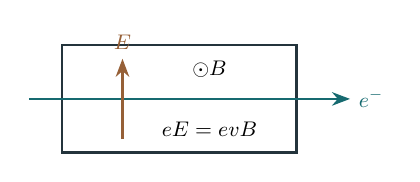
\begin{tikzpicture}[scale=.85,transform shape]

\draw[object] (-.5,-.8) rectangle (3,.8);
\draw[motion] (-1,0)--(3.8,0) node[right] {$e^-$};
\draw[force] (.4,-.6)--(.4,.6) node[above] {$E$};
\node at (1.7,.45) {$\odot B$};
\node at (1.7,-.45) {$eE=evB$};

\end{tikzpicture}
\figcaption{解图综五.2A\quad 交叉场选出速率，再以磁偏转曲率求荷质比；负号由方向判断。}
\end{minipage}\end{center}
\textbf{（1）阴极射线与电子荷质比。}
解图综五.2A中，真空放电产生的阴极射线经过狭缝形成束流。汤姆孙观察其在电场和磁场中的偏转，测出带负电粒子的荷质比，并比较不同气体和电极材料所产生的射线。它们表现出相同类型的带电粒子性质，支持电子是物质中的共同成分。

定量原理可用交叉场和平面磁偏转说明。交叉电场、磁场调到射线不偏时，电力和磁力大小相等，
\[
eE=evB,\qquad v=\frac EB.
\]
再用纯磁场中的曲率半径$r$，有$evB=mv^2/r$，故
\[
\boxed{\frac em=\frac{v}{Br}=\frac{E}{B^2r}}.
\]
这里$e$取电荷量大小，负号由偏转方向判断。测得电子的$e/m$大于氢离子相应值的千倍以上，结合随后基本电荷测量，才可分别确定很小的电子质量。荷质比只给两者的比例，结合基本电荷测量后可由$m=e/(e/m)$得到电子质量。
\begin{center}\begin{minipage}{.98\linewidth}\centering
\begin{tikzpicture}[scale=.85,transform shape]

\draw[object,line width=1.5pt] (-.5,1.1)--(2.8,1.1) (-.5,-1.1)--(2.8,-1.1);
\fill[accent] (1,0) circle (3pt) node[right] {$q$};
\draw[force] (1,0)--(1,.85) node[left] {$qE$};
\draw[force,color=warm] (1,0)--(1,-.85) node[left] {$m_{\rm eff}g$};
\node at (3.5,0) {显微观察};

\end{tikzpicture}
\figcaption{解图综五.2B\quad 重力减浮力由电力平衡；断场终速用来估计油滴尺寸。}
\end{minipage}\end{center}
\textbf{（2）油滴与电荷量子化。}
解图综五.2B的带电小油滴置于两水平极板之间，用显微镜跟踪。先断开电场，油滴向下达到终速$v_f$；重力减浮力与黏滞阻力平衡。在低雷诺数、近似球形的模型下，
\[
\frac43\pi r^3(\rho_{\rm oil}-\rho_{\rm air})g
=6\pi\eta_{\rm air}r v_f.
\]
于是由终速估计油滴半径
\[
r=\sqrt{\frac{9\eta_{\rm air}v_f}
{2(\rho_{\rm oil}-\rho_{\rm air})g}}.
\]
加电场使油滴悬浮，电力平衡有效重力，故
\[
|q|E=\frac43\pi r^3(\rho_{\rm oil}-\rho_{\rm air})g,
\qquad
|q|=\frac{6\pi\eta_{\rm air}r v_f}{E}.
\]
精密处理小油滴还需空气滑移等修正，修正后的阻力关系用于提高半径和电荷读数的准确度。

重复测不同油滴，或观察同一油滴带电量的离散改变，发现电荷量可表成$q=ne$，$n$为整数，进而测定基本电荷$e$。这一结论比“油滴会受电力”多了一层：测量显示电荷改变以共同单位发生。1910年前后的工作通过大量油滴、带电变化及阻力修正逐步提高精度，之后继续改进。
\begin{center}\begin{minipage}{.98\linewidth}\centering
\begin{tikzpicture}[scale=.85,transform shape]

\draw[object,line width=2pt] (.5,-1.2)--(.5,1.2);
\draw[motion] (-2,0)--(.4,0);
\foreach \ang in {-10,0,10,65,140}{\draw[motion] (.5,0)--++(\ang:2);}
\node[below] at (.5,-1.2) {薄箔};
\node[above] at (-1.5,.2) {$\alpha$束};

\end{tikzpicture}
\figcaption{解图综五.2C\quad 同一入射束以小角为主、极少数大角偏转，限制正电荷的空间分布。}
\end{minipage}\end{center}
\textbf{（3）大角散射与原子核。}
解图综五.2C用准直$\alpha$粒子束照射薄金属箔，通过周围可移动探测屏记录散射方向。所述厚约$10^{-6}\,\mathrm m$的薄金箔实验中，多数粒子偏转很小、绝大部分在$1^\circ$以内，约八千分之一的粒子偏转大于$90^\circ$。若正电荷弥散于整个原子，单次作用通常太弱，难以解释这种少量但显著的大角散射。

卢瑟福于1911年据此提出原子的正电荷和大部分质量集中在很小的核内，原子的大部分体积可让高速粒子近乎穿行。对足够薄的靶，以单次散射、重核近似和排斥库仑力为模型，设$\kappa_\alpha=Zze^2/(4\pi\epsilon_0)$，入射动能为$E_\alpha$、碰撞参数为$b$，有
\[
b=\frac{\kappa_\alpha}{2E_\alpha}\cot\frac\theta2,\qquad
\frac{d\sigma}{d\Omega}
=\left(\frac{\kappa_\alpha}{4E_\alpha}\right)^2
\frac1{\sin^4(\theta/2)}.
\]
角分布和能量依赖用于比较小尺度库仑中心模型与测量。实验支持核式结构，电子稳定态和能级还需相应的量子理论描述。
\begin{center}\begin{minipage}{.98\linewidth}\centering
\begin{tikzpicture}[scale=.85,transform shape]

\draw[object] (-1,-.9) rectangle (4,1);
\draw[object,line width=1.4pt] (0,-.6)--(0,.6) (2.5,-.6)--(2.5,.6) (3.5,-.6)--(3.5,.6);
\draw[motion] (.3,0)--(2.2,0);
\node[above] at (.8,1) {汞蒸气};
\node[below] at (1.3,-.9) {加速$U$};
\node[right] at (4.1,.2) {收集};

\end{tikzpicture}
\figcaption{解图综五.2D\quad 加速区、汞蒸气与反向收集区使离散能量损失显示为电流下降。}
\end{minipage}\end{center}
\textbf{（4）非弹性碰撞与离散激发能。}
解图综五.2D中，电子被加速电压$U$加速，穿过汞蒸气，再克服一个小反向电势到达收集极。随着$U$增大，收集电流随电压总体上升，并在近似等间距电压处反复出现下降。

在汞的典型实验条件下，间距约$4.9\,\mathrm V$。当电子获得足够动能，可通过非弹性碰撞把约$4.9\,\mathrm{eV}$交给一个汞原子，自己损失这部分能量，因而有些电子在反向场中折返，收集电流随之下降。电压再提高，电子可在到达前发生两次、三次这样的能量损失，于是形成重复结构。
\[
\Delta E=e\,\Delta U,\qquad
\Delta U\simeq4.9\,\mathrm V.
\]
这说明原子吸收的激发能不是任意连续值，而有确定的能级差。若将该能量以一个光子释放，波长约为
$hc/\Delta E\simeq253\,\mathrm{nm}$。电流峰谷的绝对位置还受接触电势、温度和碰撞位置影响；相邻间距比单个峰位置更直接反映激发能。这一结果与玻尔模型中离散定态的核心假设相符，实验直接测得的是确定的激发能差。
\begin{center}\begin{minipage}{.98\linewidth}\centering
\begin{tikzpicture}[scale=.85,transform shape]

\fill (0,0) circle (2pt) node[left] {$\odot$扭轴};
\draw[object] (0,0)--(2,0);
\draw[object,line width=2pt] (1.6,0)--(2.4,0);
\draw[motion] (1.8,-1)--(1.8,-.1);
\draw[motion] (2.1,-1)--(2.1,-.1);
\draw[force] (2,.1)--(2,1.4) node[right] {$F$};
\draw[guide] (.6,0) arc[start angle=0,end angle=40,radius=.6];
\node at (.8,.6) {扭角};
\node at (1,-1.4) {俯视：光束沿纸面入射};

\end{tikzpicture}
\figcaption{解图综五.2E\quad 辐射给薄片动量，扭丝回复力矩平衡微小光压。}
\end{minipage}\end{center}
\textbf{（5）光压与辐射动量。}
解图综五.2E把薄片悬在灵敏扭秤上，光照后由扭转角估计作用力。列别捷夫与尼科尔斯、赫尔的研究测量了很小的辐射压力，并处理热效应、残余气体等影响，确认光可以向物体传递动量。

若光束以强度$I$正入射，完全吸收时每单位时间、单位面积传递能量$I$及动量$I/c$，压力为
\[
p_{\rm abs}=\frac Ic.
\]
完全镜面反射使法向动量反向，改变为两倍，故$p_{\rm refl}=2I/c$。受照面积$A$对应力$F=pA$，扭矩再与扭秤回复力矩平衡。这是光携带动量的直接测量，经典电磁理论和光子描述均给出光压；康普顿散射中的角度依赖波长位移进一步呈现单次光子碰撞的关系。
\begin{center}\begin{minipage}{.98\linewidth}\centering
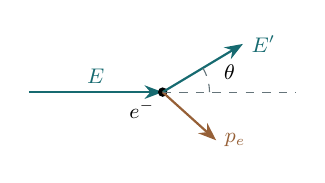
\begin{tikzpicture}[scale=.85,transform shape]

\draw[motion] (-2,0)--(0,0) node[midway,above] {$E$};
\fill (0,0) circle (2pt) node[below left] {$e^-$};
\draw[motion] (0,0)--(1.2,.72) node[right] {$E'$};
\draw[force] (0,0)--(.8,-.72) node[right] {$p_e$};
\draw[guide] (0,0)--(2,0);
\draw[guide] (.7,0) arc[start angle=0,end angle=30.96,radius=.7];
\node at (1,.3) {$\theta$};

\end{tikzpicture}
\figcaption{解图综五.2F\quad 光子散射方向与电子反冲共同满足能量动量守恒。}
\end{minipage}\end{center}
\textbf{（6）康普顿波长位移。}
解图综五.2F中，以X射线照射石墨等物质并测不同散射角$\theta$的光谱。散射谱中出现比入射波长更长的分量，其位移随角度变化。用光子与近似自由、起初静止电子碰撞，可由能量和动量守恒解释。

设入射、散射光子能量分别为$E,E'$，电子反冲动量为$\boldsymbol p_e$。守恒式为
\[
E+m_ec^2=E'+\sqrt{m_e^2c^4+p_e^2c^2},
\quad
\boldsymbol p_e=\frac Ec\hat{\boldsymbol n}
-\frac{E'}c\hat{\boldsymbol n}'.
\]
动量式平方给$p_e^2c^2=E^2+E'^2-2EE'\cos\theta$；能量式移项平方则给
$p_e^2c^2=(E-E')^2+2m_ec^2(E-E')$。相减得到
\[
EE'(1-\cos\theta)=m_ec^2(E-E').
\]
再用$E=hc/\lambda,E'=hc/\lambda'$，
\[
\boxed{\lambda'-\lambda=\frac{h}{m_ec}(1-\cos\theta)}.
\]
该角度规律不取决于照射强度，支持光子的能量—动量描述。近自由、初始静止电子是此式的条件；束缚电子或整体物体的散射可产生不同分量，谱中各分量需按相应反冲模型解释。
\begin{center}\begin{minipage}{.98\linewidth}\centering
\begin{tikzpicture}[scale=.85,transform shape]

\foreach \y in {0,-.5,-1}{\draw[object] (-2,\y)--(2,\y);}
\draw[motion] (-2,1.3)--(0,0);
\draw[motion] (0,0)--(2,1.3) node[right] {峰方向};
\draw[guide] (.8,0) arc[start angle=0,end angle=33,radius=.8];
\node at (1.2,.3) {$\theta_B$};
\node[left] at (-2,-.25) {$d$};

\end{tikzpicture}
\figcaption{解图综五.2G\quad 布拉格角相对晶面定义，峰位置须和实际探测角换算。}
\end{minipage}\end{center}
\textbf{（7）晶体电子衍射与物质波。}
解图综五.2G中，具有已知加速能量的电子束照射镍单晶，探测器测电子强度随方向的变化。某些方向出现显著峰值，并随电子能量和晶体方向改变，与波的相干衍射相符。

电子加速电压为$U$，在非相对论范围内$p=\sqrt{2m_eeU}$，德布罗意波长
\[
\lambda=\frac hp=\frac{h}{\sqrt{2m_eeU}}.
\]
晶面间距$d$已知时，布拉格干涉条件为$2d\sin\theta_B=n\lambda$，其中$\theta_B$是束流与晶面的掠射角，探测器报告角依其入射、出射方向定义换算后使用。由角分布反推的波长与$h/p$一致，证实电子的波动性。例如$U=54\,\mathrm V$给$\lambda\simeq0.167\,\mathrm{nm}$，与晶体原子尺度相当，所以可见明显衍射。
\begin{center}\begin{minipage}{.98\linewidth}\centering
\begin{tikzpicture}[scale=.85,transform shape]

\coordinate (O) at (0,0);
\draw[object] (-1,0)--(2,0) (0,-1)--(0,2);
\draw[object,line width=2pt] (2,-.4)--(2,.4) (-.4,2)--(.4,2);
\draw[object,line width=1.3pt] (-.4,-.4)--(.4,.4);
\draw[motion] (-1,0)--(-.5,0);
\draw[motion] (.4,.15)--(1.7,.15);
\draw[motion] (.15,.4)--(.15,1.7);
\node[below] at (1,0) {$L$};\node[left] at (0,1) {$L$};
\node at (2,-1) {转90度比较条纹};

\end{tikzpicture}
\figcaption{解图综五.2H\quad 等长正交臂分束后重新干涉，转动装置比较方向相关的往返时间差。}
\end{minipage}\end{center}
\textbf{（8）正交光臂与以太风预言。}
解图综五.2H将同一光束分到两条正交光臂，反射后重合干涉，并将装置转动以比较条纹。1887年的合作实验在1881年先前尝试的基础上提高了灵敏度。

在作为比较对象的简单静止以太模型中，若装置相对以太以$v$运动，取两臂单程等效长度均为$L$、以太中光速$c$，平行臂往返时间为
\[
t_\parallel=\frac L{c-v}+\frac L{c+v}
=\frac{2Lc}{c^2-v^2}.
\]
垂直臂要随装置横移，往返时间为
$t_\perp=2L/\sqrt{c^2-v^2}$。在$v\ll c$下，
\[
t_\parallel-t_\perp\simeq\frac{Lv^2}{c^3}.
\]
装置转$90^\circ$使两臂交换角色，预期时间差改变两倍，对应条纹移动数
\[
\Delta n\simeq\frac{2Lv^2}{\lambda c^2}.
\]
实际未发现与该预期相符的明显周期性移动。这一零结果约束了上述简单以太风模型，是后来相对论发展的实验背景之一。狭义相对论以真空光速与惯性系规律的一致性解释它；该实验直接比较的是光的往返传播，相对性原理涉及更广的物理规律和实验事实；不同介质假设则按各自的传播预言与实验比较。


\Needspace{13\baselineskip}

\pdfbookmark[2]{第 3 题 双珠滑环的张力与上升阈值}{q3}

\section*{第 3 题\quad 双珠滑环的张力与上升阈值}\label{q:3}


质量$M$、半径$R$的刚性圆环用不可伸长轻绳悬挂，两颗质量均为$m$的小珠穿在圆环上，可沿环无摩擦运动，约束能向珠施加径向推力或拉力。两珠从顶端附近经微小对称扰动后向两侧滑下，取初始动能趋于零、起点趋于顶端的极限。

（1）在圆环仍静止的条件下，画悬绳张力$T$随$x=\cos\theta$变化的曲线，求形式上的极小值。$\theta$从竖直向上的半径量起，$-1\le x\le1$。

（2）求圆环能实际离开静止位置向上运动的质量比条件，并画临界情形的张力曲线。区分张力瞬时为零与出现有限上升这两种情形，求超过阈值时首次松绳的角度。


\begin{center}\begin{minipage}{.98\linewidth}\centering
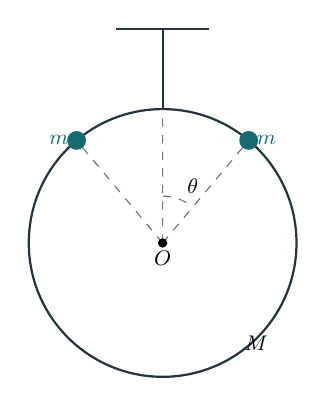
\begin{tikzpicture}[scale=.85,transform shape]

\draw[object] (0,0) circle (2);
\draw[object] (0,2)--(0,3.2);
\draw[object] (-.7,3.2)--(.7,3.2);
\fill[accent] (50:2) circle (4pt) node[right] {$m$};
\fill[accent] (130:2) circle (4pt) node[left] {$m$};
\draw[guide] (0,0)--(50:2) (0,0)--(130:2) (0,0)--(0,2);
\draw[guide] (0,.7) arc[start angle=90,end angle=50,radius=.7];
\node at (.45,.85) {$\theta$};
\fill (0,0) circle (2pt) node[below] {$O$};
\node at (1.4,-1.5) {$M$};

\end{tikzpicture}
\figcaption{图综五.3\quad 两珠穿环形成双向约束，悬绳只能提供向上拉力。}
\end{minipage}\end{center}

\Needspace{6\baselineskip}\subsection*{解答}


图综五.3的两颗珠始终穿在环上，径向约束可以改变符号。两珠精确位于顶点且速度为零时，理想系统有静止平衡解；以下取微小对称扰动后开始滑动、起点趋于顶端且初始能量趋于零的极限。
\begin{center}\begin{minipage}{.98\linewidth}\centering
\begin{tikzpicture}[scale=.8,transform shape]

\draw[object] (0,0) circle (2);
\fill (1,1.732) circle (4pt) node[right] {右珠};
\draw[guide] (0,0)--(1,1.732);
\draw[force] (1,1.732)--(1.5,2.598) node[above] {$N>0$向外};
\draw[force,color=warm] (1,1.732)--(1,.45) node[right] {$mg$};
\begin{scope}[xshift=6cm]
\draw[object] (0,0) circle (1.3);
\draw[force] (0,1.3)--(0,2.7) node[above] {$T$};
\draw[force,color=warm] (0,0)--(0,-1.5) node[below] {$Mg$};
\draw[force] (.65,1.126)--(.15,.26);
\draw[force] (-.65,1.126)--(-.15,.26);
\node at (0,-2.5) {两珠反作用竖分量合为$-2Nx$};
\end{scope}

\end{tikzpicture}
\figcaption{解图综五.3A\quad 珠的径向力与环的反作用分开列式；$N<0$时环向内拉珠。}
\end{minipage}\end{center}
解图综五.3A先把环看作静止。小珠从顶端下降高度$R(1-\cos\theta)$，能量守恒给
\[
\frac12mv^2=mgR(1-\cos\theta),\qquad
v^2=2gR(1-x).
\]
规定环对珠的径向向外约束力为$N$，径向向内列牛顿方程：
\[
mg\cos\theta-N=\frac{mv^2}{R},
\qquad
\boxed{N=mg(3x-2)}.
\]
所以$x>2/3$时$N>0$，环向外推珠；$x<2/3$时$N<0$，环向内拉珠。由于珠穿在环上，$N<0$表示环向内拉珠，穿环约束仍成立。

两珠对环的水平反力相消，竖直反力之和为$-2Nx$。环仍静止时有
\[
T-Mg-2Nx=0,
\]
因而
\[
\boxed{T_{\rm fixed}(x)=Mg+2mg(3x^2-2x)
=Mg-\frac23mg+6mg\left(x-\frac13\right)^2}.
\]
由抛物线顶点，
\[
\boxed{x_{\min}=\frac13,\quad
\theta_{\min}=\arccos\frac13\simeq70.53^\circ,\quad
T_{\min}=Mg-\frac23mg}.
\]
\begin{center}\begin{minipage}{.98\linewidth}\centering
\begin{tikzpicture}[scale=.8,transform shape]

\draw[axis] (-3,0)--(3.6,0) node[right] {$x=\cos\theta$};
\draw[axis] (0,-1)--(0,6.2) node[above] {$T_{\rm fixed}/Mg$};
\draw[traj,domain=-1:1,samples=120] plot ({3*\x},{.18*(1+2*(3*\x*\x-2*\x))});
\draw[guide,color=warm,domain=-1:1,samples=120] plot ({3*\x},{.18*(1+6*(3*\x*\x-2*\x))});
\node[below] at (-3,0) {$-1$};\node[below] at (3,0) {$1$};
\node[left] at (0,.18) {$1$};
\node[text=accent] at (4.8,1.5) {$m/M=1$};
\node[text=warm] at (4.8,3) {$m/M=3$};
\node at (1.5,-1.8) {虚线负段给维持环固定所需的向下作用；松绳后$T=0$};

\end{tikzpicture}
\figcaption{解图综五.3B\quad 固定环所需张力是抛物线；曲线穿零后转入松绳运动。}
\end{minipage}\end{center}
解图综五.3B画的是“环固定”假设所需的张力。轻绳沿绳向上拉环，实际张力满足$T\ge0$；当$T_{\rm fixed}<0$时，维持环固定需要向下作用，环因而转入松绳运动。若$m/M<3/2$，整条曲线为正，绳可保持绷紧，圆环不必上升。

临界$m/M=3/2$时
\[
\boxed{T_{\rm crit}=Mg(3x-1)^2}.
\]
解图综五.3C中的抛物线在$x=1/3$处与横轴相切；$x=1$时$T=4Mg$，$x=-1$时$T=16Mg$。这个临界系统只在一个瞬间需要零张力，之后仍需要正张力，保持环静止始终满足单边约束。因此临界比是实际上升条件的下确界；在精确理想模型下，等号本身不产生有限上升。
\begin{center}\begin{minipage}{.98\linewidth}\centering
\begin{tikzpicture}[scale=.8,transform shape]

\draw[axis] (-3,0)--(3.6,0) node[right] {$x$};
\draw[axis] (0,0)--(0,5.5) node[above] {$T/Mg$};
\draw[traj,domain=-1:1,samples=160] plot ({3*\x},{.3*(3*\x-1)^2});
\draw[guide] (1,0)--(1,1.3);
\node[below] at (1,0) {$1/3$};
\node[below] at (-3,0) {$-1$};\node[below] at (3,0) {$1$};
\draw[guide] (-3,4.8)--(0,4.8) node[right] {$16$};
\draw[guide] (0,1.2)--(3,1.2);\node[left] at (0,1.2) {$4$};
\node at (4.8,3.5) {$T=Mg(3x-1)^2$};
\node at (4.8,2.3) {$m/M=3/2$};
\node at (1.5,-1.3) {临界仅瞬时触零；实际上升须$m/M>3/2$};

\end{tikzpicture}
\figcaption{解图综五.3C\quad 临界曲线与横轴相切，触零与有限上升不是同一条件。}
\end{minipage}\end{center}
实际向上离开悬挂位置要求一段运动中固定环公式需负张力，即
\[
\boxed{\frac mM>\frac32}.
\]
随着珠下滑，$x$从1减小，首次到达$T_{\rm fixed}=0$的是二次方程的较大根：
\[
3x^2-2x+\frac{M}{2m}=0,\qquad
\boxed{x_+=\frac{1+\sqrt{1-3M/(2m)}}3}.
\]
故首次松绳角为
\[
\boxed{\theta_{\rm lift}=\arccos x_+}.
\]
刚过此角时，珠对环的向上作用超过环重，绳松弛、$T=0$，圆环获得向上加速度；此后环会运动，珠的能量及约束方程都须重新写，固定环抛物线只提供首次松绳的初值，之后由珠与环的耦合运动确定。令$m/M\to(3/2)^+$，首次松绳角趋向$70.53^\circ$，这才是临界角的上升极限含义。

\textbf{首次松绳后的向上运动。} 为把负张力区与实际运动联系起来，解图综五.3D将圆环中心的竖直位移记为$Y$，向上取正。两珠相对中心的坐标分别为$(\pm R\sin\theta,R\cos\theta)$，所以惯性系中的位置是$(\pm R\sin\theta,Y+R\cos\theta)$。对两颗珠一起计算，动能和势能分别为
\[
K=\frac12(M+2m)\dot Y^2-2mR\sin\theta\,\dot Y\dot\theta
+mR^2\dot\theta^2,\qquad
V=(M+2m)gY+2mgR\cos\theta.
\]
交叉项来自珠的竖直速度$\dot Y-R\sin\theta\,\dot\theta$；它具体说明了环运动后珠速与固定环计算的区别。
\begin{center}\begin{minipage}{.98\linewidth}\centering
\begin{tikzpicture}[scale=0.72,transform shape]
\draw[object] (0,.5) circle (2);
\draw[guide] (-2.6,0)--(2.6,0);
\fill (0,.5) circle (2pt) node[below right] {$C$};
\draw[guide] (0,.5)--(0,2.5);
\foreach \x in {-1.7320508,1.7320508}{\fill[accent] (\x,1.5) circle (3pt);\draw[guide] (0,.5)--(\x,1.5);}
\draw[guide] (0,1.2) arc[start angle=90,end angle=30,radius=.7];
\node at (.65,1.3) {$\theta$};
\draw[motion] (-3.1,0)--(-3.1,.5) node[midway,left] {$Y$};
\node[align=left] at (5,.5) {两珠坐标\\$(\pm R\sin\theta,Y+R\cos\theta)$\\$\dot z=\dot Y-R\sin\theta\,\dot\theta$};
\node[below] at (0,-1.7) {松绳后以环中心平动与珠相对运动共同描述};\end{tikzpicture}
\figcaption{解图综五.3D\quad 环中心上移与珠在环上滑动共同进入惯性系速度}
\end{minipage}\end{center}
对$Y,\theta$分别写动力学关系，得到
\[
(M+2m)\ddot Y-2mR(\sin\theta\,\ddot\theta+
\cos\theta\,\dot\theta^2)=T-(M+2m)g,
\quad
R\ddot\theta=(g+\ddot Y)\sin\theta.
\]
松绳时取$T=0$，消去$\ddot\theta$得
\[
\ddot Y=-g+
\frac{2mR\cos\theta\,\dot\theta^2}{M+2m\cos^2\theta}.
\]
首次松绳恰在$x=x_+$，当时环尚未移动，$\dot Y=0$、$R\dot\theta^2=2g(1-x_+)$。代入可见$\ddot Y=0$：约束转换瞬间的加速度也连续，向上运动由随后变化的珠位置与速度产生。

令$t_*$为首次松绳时刻。在它的右侧，$\theta,\dot\theta$起初与固定环过程有相同的一阶变化，所以
\[
Y^{(3)}(t_*+)
=-\frac{\dot T_{\rm fixed}(t_*)}{M+2mx_+^2}.
\]
超阈值时$x_+>1/3$，$dT_{\rm fixed}/dx=12mg(x_+-1/3)>0$，而$\dot x=-\sin\theta\,\dot\theta<0$，故$\dot T_{\rm fixed}<0$，上式严格为正。因而短时位移为
\[
Y(t_*+\Delta t)
=-\frac{\dot T_{\rm fixed}(t_*)}{6(M+2mx_+^2)}
(\Delta t)^3+O((\Delta t)^4)>0.
\]
这给出严格质量比$m/M>3/2$下确有一段向上运动的局部证明。在等号处，两根合并且$\dot T_{\rm fixed}=0$，固定环解的张力始终非负，与悬绳的条件一致；临界点只提供向上运动的极限阈值。


\Needspace{13\baselineskip}

\pdfbookmark[2]{第 4 题 一维气体绝热压缩的微观推导}{q4}

\section*{第 4 题\quad 一维气体绝热压缩的微观推导}\label{q:4}


柱形容器内有大量质量相同的小球，只沿容器长度方向往返运动，小球看作质点，彼此及与端面均作弹性正碰。速率和方向杂乱，以平均动能定义“温度”
\[
\overline\varepsilon=\frac12k_{\rm B}T.
\]
一端装有平面弹性活塞，沿容器长度方向缓慢向内推进。容器截面积固定，忽略重力和各种阻力，过程无热量交换。

从与移动活塞的碰撞出发，导出$T$与容积$V$的关系；说明相同质量小球间碰撞的作用，并用热容比及热力学第一定律分别推导同一关系。讨论范围是准静态压缩极限。


\begin{center}\begin{minipage}{.98\linewidth}\centering
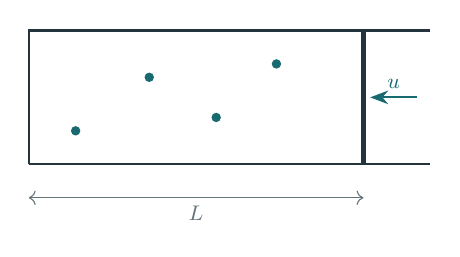
\begin{tikzpicture}[scale=.85,transform shape]

\draw[object] (0,0)--(0,2)--(6,2) (0,0)--(6,0);
\draw[object,line width=2pt] (5,0)--(5,2);
\foreach \x/\y in {.7/.5,1.8/1.3,2.8/.7,3.7/1.5}{\fill[accent] (\x,\y) circle (2pt);}
\draw[motion] (5.8,1)--(5.1,1) node[midway,above] {$u$};
\draw[axis,<->] (0,-.5)--(5,-.5) node[midway,below] {$L$};

\end{tikzpicture}
\figcaption{图综五.4\quad 一维质点只沿柱轴运动，活塞向内缓慢推进，截面积保持不变。}
\end{minipage}\end{center}

\Needspace{6\baselineskip}\subsection*{解答}


图综五.4把轴线向右定为正，右端活塞以速度$-u$向左推进，$u>0$，容器瞬时长度为$L$。准静态极限要求一次往返期间长度改变很小，对所跟踪速率$v$有$u\ll v$。
\begin{center}\begin{minipage}{.98\linewidth}\centering
\begin{tikzpicture}[scale=.82,transform shape]

\node at (1,2) {同质量球交换速度};
\fill (0,1) circle (3pt);\fill (2,1) circle (3pt);
\draw[motion] (0,1.3)--(1.3,1.3) node[midway,above] {$v_1$};
\draw[motion] (2,.7)--(1,.7) node[midway,below] {$v_2$};
\node at (1,-.3) {$v'_1=v_2,\quad v'_2=v_1$};
\begin{scope}[xshift=6cm]
\draw[object,line width=2pt] (2,-.5)--(2,2);
\draw[motion] (-.5,1.3)--(1.7,1.3) node[midway,above] {$v$};
\draw[motion] (1.7,.3)--(-.5,.3) node[midway,below] {$v+2u$};
\draw[motion] (2.8,1)--(2.1,1) node[above] {$-u$};
\end{scope}

\end{tikzpicture}
\figcaption{解图综五.4A\quad 速度携带者等效穿行；移动壁反射使地面系速率增加$2u$。}
\end{minipage}\end{center}
解图综五.4A中，两个同质量质点弹性正碰，动量与动能守恒：
\[
v_1+v_2=v'_1+v'_2,\qquad
v_1^2+v_2^2=v_1'^2+v_2'^2.
\]
非平凡碰撞解是$v'_1=v_2,v'_2=v_1$，即交换速度。若跟踪的不是某颗球而是某个速度的“携带者”，碰撞看起来是两条速度轨迹穿过彼此，因而可以跟踪它们在两壁间的往返。

一颗向右速率$v$的小球追上活塞，在活塞参考系中入射速度为$v+u$，弹性反射后为$-(v+u)$；变回地面系，再加活塞速度$-u$，
\[
v'_{\rm lab}=-(v+2u).
\]
因而每次与活塞相碰后速率增加$\Delta v=2u$，增加的动能由推动活塞的外力提供。
\textbf{一次碰撞怎样传递能量。} 图A中的地面系速度改变由相对速度反射与加回壁速两步组成。若入射速度为$v$，出射速度为$-(v+2u)$，单次动能增加
\[
\Delta\varepsilon=\frac m2[(v+2u)^2-v^2]
=2muv+2mu^2.
\]
向右取正，活塞对球的冲量为$\Delta p=-2m(v+u)$；恒定壁速为$-u$，碰撞功$(-u)\Delta p=2muv+2mu^2$，与球的动能增量相等。低阶每碰增加$2muv$，乘往返碰撞频率$v/(2L)$，功率为$mu v^2/L$；这也等于平均力$mv^2/L$乘推进速率$u$。微观能量增加与宏观外力做功由同一个碰撞过程联系起来。

\begin{center}\begin{minipage}{.98\linewidth}\centering
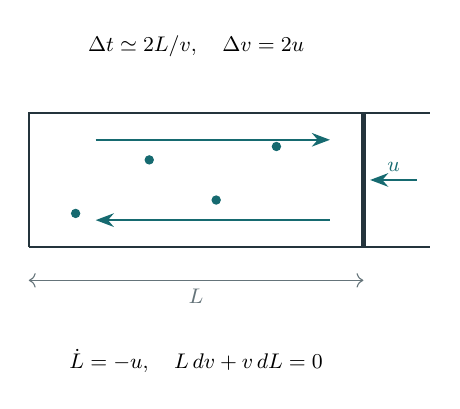
\begin{tikzpicture}[scale=.85,transform shape]

\draw[object] (0,0)--(0,2)--(6,2) (0,0)--(6,0);
\draw[object,line width=2pt] (5,0)--(5,2);
\foreach \x/\y in {.7/.5,1.8/1.3,2.8/.7,3.7/1.5}{\fill[accent] (\x,\y) circle (2pt);}
\draw[motion] (5.8,1)--(5.1,1) node[midway,above] {$u$};
\draw[axis,<->] (0,-.5)--(5,-.5) node[midway,below] {$L$};

\draw[motion] (1,1.6)--(4.5,1.6);
\draw[motion] (4.5,.4)--(1,.4);
\node at (2.5,3) {$\Delta t\simeq2L/v,\quad\Delta v=2u$};
\node at (2.5,-1.7) {$\dot L=-u,\quad L\,dv+v\,dL=0$};

\end{tikzpicture}
\figcaption{解图综五.4B\quad 两次遇同一活塞需要往返；速度与长度共同给绝热不变量。}
\end{minipage}\end{center}
解图综五.4B将连续碰撞与缓慢缩短联系起来。一个速度携带者两次碰到右端活塞之间，往返时间在一阶近似下为$\Delta t\simeq2L/v$。于是
\[
\frac{dv}{dt}\simeq\frac{2u}{2L/v}=\frac{uv}{L},
\qquad \frac{dL}{dt}=-u.
\]
消去时间，得到
\[
L\,dv+v\,dL=0,\qquad \boxed{vL=\text{常量}}.
\]
它是准静态极限的绝热不变量；连续近似采用$u/v\to0$；快速壁运动按每次精确反射和实际碰撞时刻逐次计算。

对单个携带者，$\varepsilon=mv^2/2$，有$d\varepsilon=mv\,dv$，故
\[
L\,d\varepsilon+2\varepsilon\,dL=0.
\]
因为所有速度携带者都在同一瞬时长度下缩放，对它们取平均：
\[
L\,d\overline\varepsilon+2\overline\varepsilon\,dL=0.
\]
取平均时，每个速度携带者都满足$d(v_i^2L^2)=0$，因此
\[
\langle v^2\rangle L^2
=\frac1N\sum_i v_i^2L^2=\text{常量}.
\]
这里各携带者的速率可以不同，求和只用到所有项具有相同的长度缩放因子。两球碰撞交换速度而不改变速率集合，球的身份变化与这个平均无关。

代$\overline\varepsilon=k_{\rm B}T/2$，
\[
L\,dT+2T\,dL=0,\qquad
\frac{dT}T+2\frac{dL}L=0.
\]
截面积$A$不变，$V=AL$，所以
\[
\boxed{TV^2=T_0V_0^2=\text{常量}}.
\]
容积缩小到一半，温度变为四倍。相同质量的一维碰撞只交换速度并保留速率集合，任意初始分布可保持非平衡形状；题设以平均动能定义的温度已足够上述推导。若初态为高斯平衡分布，准静态的统一速度缩放保持其形状。
\begin{center}\begin{minipage}{.98\linewidth}\centering
\begin{tikzpicture}[scale=.85,transform shape]

\draw[axis] (0,0)--(5.7,0) node[right] {$V/V_0$};
\draw[axis] (0,0)--(0,4.6) node[above] {$T/T_0$};
\draw[traj,domain=.5:2,samples=100] plot ({2.5*\x},{1/(\x*\x)});
\draw[guide] (1.25,0)--(1.25,4)--(0,4);
\node[below] at (1.25,0) {$1/2$};\node[left] at (0,4) {$4$};
\draw[guide] (2.5,0)--(2.5,1)--(0,1);
\node[below] at (2.5,0) {$1$};\node[left] at (0,1) {$1$};
\node[align=left] at (7,2) {$TV^2=\text{常量}$\\$pV^3=\text{常量}$\\$\gamma=3$};

\end{tikzpicture}
\figcaption{解图综五.4C\quad 一维平均动能温度随体积平方反比变化，对应一个轴向平动自由度和$\gamma=3$。}
\end{minipage}\end{center}
解图综五.4C再从宏观量理解同一关系。质量$m$、速率$v$的一个携带者每次碰固定壁给壁冲量$2mv$，碰壁频率$v/(2L)$，故其平均力为$mv^2/L$。对$N$个球相加，
\[
pA=\frac{Nm\langle v^2\rangle}{L},\qquad
pV=Nm\langle v^2\rangle=Nk_{\rm B}T.
\]
本题的质点没有内部转动或振动能量，能量中只有一个轴向平动平方项。若按每个二次项贡献$k_{\rm B}T/2$记数，平动贡献为1、转动和振动贡献均为0，故总数为1，得到$C_V=Nk_{\rm B}/2$。状态方程使焓$U+pV=3Nk_{\rm B}T/2$，定压热容由其温度导数得到$C_p=3Nk_{\rm B}/2$。热容比法和第一定律法正是把同一能量约定写成宏观形式。

一维质点只有一个平动自由度，
\[
U=\frac12Nk_{\rm B}T,\quad
C_V=\frac12Nk_{\rm B},\quad
C_p=C_V+Nk_{\rm B}=\frac32Nk_{\rm B}.
\]
故$\gamma=C_p/C_V=3$，可逆绝热关系$TV^{\gamma-1}=\text{常量}$再次给$TV^2=\text{常量}$。三维单原子气体的$\gamma=5/3$对应三个平动二次项，本题采用一个轴向平动项。

最后直接用第一定律。无热交换，外界对气体做功为$-p\,dV$，因此
\[
dU=-p\,dV,\qquad
\frac12Nk_{\rm B}\,dT
=-\frac{Nk_{\rm B}T}{V}\,dV.
\]
约去常数并积分，
\[
\frac{dT}T=-2\frac{dV}V,\qquad
\ln\frac T{T_0}=-2\ln\frac V{V_0}.
\]
仍得$TV^2=T_0V_0^2$；结合$pV=Nk_{\rm B}T$，还可写$pV^3=\text{常量}$。三种方法中的温度、内能和自由度约定一致。


\Needspace{13\baselineskip}

\pdfbookmark[2]{第 5 题 直流导线中的电磁能流与焦耳热}{q5}

\section*{第 5 题\quad 直流导线中的电磁能流与焦耳热}\label{q:5}


一根无限长、圆截面的均匀直导线，半径为$R$，电导率为$\sigma$，通有沿轴向$+z$的恒定电流$I$。电流密度在截面上均匀。

（1）指出导线内坡印廷矢量（能流密度）的方向，并求随径向距离$r$的分布。（2）计算单位时间经长$l$的一段导线表面流入的能量。（3）证明它等于这段导线的焦耳热功率，并说明局部能量守恒。采用$\boldsymbol S=\boldsymbol E\times\boldsymbol H$。


\begin{center}\begin{minipage}{.98\linewidth}\centering
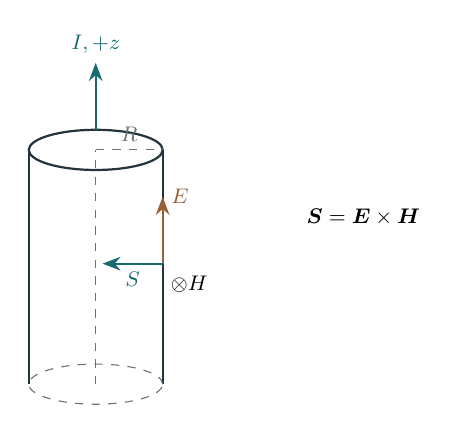
\begin{tikzpicture}[scale=.85,transform shape]

\draw[object] (-1,0)--(-1,3.5) (1,0)--(1,3.5);
\draw[object] (0,3.5) ellipse (1 and .3);
\draw[guide] (0,0) ellipse (1 and .3);
\draw[motion] (0,3.8)--(0,4.8) node[above] {$I,+z$};
\draw[guide] (0,0)--(0,3.5);
\draw[guide] (0,3.5)--(1,3.5) node[midway,above] {$R$};

\draw[force] (1,1.8)--(1,2.8) node[right] {$E$};
\node[right] at (1,1.5) {$\otimes H$};
\draw[motion] (1,1.8)--(.1,1.8) node[midway,below] {$S$};
\node at (4,2.5) {$\boldsymbol S=\boldsymbol E\times\boldsymbol H$};

\end{tikzpicture}
\figcaption{图综五.5\quad 电流沿轴向，电场轴向、磁场环向，能流从侧面径向流入。}
\end{minipage}\end{center}

\Needspace{6\baselineskip}\subsection*{解答}


图综五.5用柱坐标$(r,\varphi,z)$描述导线，电流沿$+z$。稳恒均匀欧姆导体内，
\[
\boldsymbol j=\frac{I}{\pi R^2}\hat{\boldsymbol e}_z,\qquad
\boldsymbol E=\frac{\boldsymbol j}{\sigma}
=\frac{I}{\sigma\pi R^2}\hat{\boldsymbol e}_z.
\]
\begin{center}\begin{minipage}{.98\linewidth}\centering
\begin{tikzpicture}[scale=.85,transform shape]

\draw[axis] (0,0)--(3.4,0) node[right] {$\hat{\boldsymbol e}_r$};
\draw[axis] (0,0)--(0,3.1) node[above] {$E\hat{\boldsymbol e}_z$};
\node[below] at (1.5,.6) {$\otimes H\hat{\boldsymbol e}_\varphi$};
\draw[force] (0,1.3)--(-2,1.3) node[left] {$\boldsymbol S$};
\node at (1,-1) {$\hat{\boldsymbol e}_z\times\hat{\boldsymbol e}_\varphi=-\hat{\boldsymbol e}_r$};

\end{tikzpicture}
\figcaption{解图综五.5A\quad 在导线右侧一点确定三个方向，柱坐标基矢采用同一右手系。}
\end{minipage}\end{center}
解图综五.5A的磁场环绕轴线，右手方向为$+\varphi$。在$r<R$处取同轴圆形安培回路，所包电流为$I r^2/R^2$，因此
\[
H_\varphi(r)\,2\pi r=I\frac{r^2}{R^2},
\qquad
\boxed{\boldsymbol H=\frac{Ir}{2\pi R^2}\hat{\boldsymbol e}_\varphi}.
\]
柱坐标基矢满足$\hat{\boldsymbol e}_z\times\hat{\boldsymbol e}_\varphi
=-\hat{\boldsymbol e}_r$，所以
\[
\boxed{\boldsymbol S(r)=
-\frac{I^2r}{2\sigma\pi^2R^4}\hat{\boldsymbol e}_r,\qquad0\le r\le R}.
\]
能流径向指向导线内部，轴线上因磁场为零而$\boldsymbol S=0$。本段的焦耳耗散由周围电磁场经侧面连续输入，方向由轴向电场与环向磁场的叉乘确定。
\textbf{侧面能量与表面场。} 图B积分的是进入导体的法向功率，因此也可从表面外侧的场来算。稳恒电场满足$\nabla\times\boldsymbol E=0$，跨过导体表面取一个窄矩形回路，可得轴向切向电场连续，$E_{z,\rm out}=E_{z,\rm in}=I/(\sigma\pi R^2)$。电流在截面内连续分布，表面没有额外的理想面电流，环向磁场的两侧极限也一致，$H_\varphi(R)=I/(2\pi R)$。所以紧贴表面外侧的径向能流同样为$-E_zH_\varphi$，与内部算出的流入值相接。

\begin{center}\begin{minipage}{.98\linewidth}\centering
\begin{tikzpicture}[scale=.85,transform shape]

\draw[object] (-1,0)--(-1,3.5) (1,0)--(1,3.5);
\draw[object] (0,3.5) ellipse (1 and .3);
\draw[guide] (0,0) ellipse (1 and .3);
\draw[motion] (0,3.8)--(0,4.8) node[above] {$I,+z$};
\draw[guide] (0,0)--(0,3.5);
\draw[guide] (0,3.5)--(1,3.5) node[midway,above] {$R$};

\foreach \y in {.7,1.5,2.3,3.1}{
\draw[force] (-2,\y)--(-1.05,\y);
\draw[force] (2,\y)--(1.05,\y);}
\draw[axis,<->] (2.8,0)--(2.8,3.5) node[midway,right] {$l$};
\node at (5,2) {$P_{\rm in}=2\pi RlS_R$};
\node at (5,1) {端面通量为零};

\end{tikzpicture}
\figcaption{解图综五.5B\quad 同一段导线的能量经整个侧面输入，向外法向通量为负。}
\end{minipage}\end{center}
解图综五.5B在表面$r=R$有
\[
S_R=\frac{I^2}{2\sigma\pi^2R^3}.
\]
长$l$一段导线侧面积为$2\pi Rl$，且向外法线为$+\hat{\boldsymbol e}_r$，流入功率为负的向外通量：
\[
\boxed{P_{\rm in}=-\int_{\rm side}\boldsymbol S\cdot d\boldsymbol A
=2\pi RlS_R=\frac{I^2l}{\sigma\pi R^2}}.
\]
两端面法线沿$\pm z$，能流沿径向，与端面法线垂直，故端面通量为零。
\begin{center}\begin{minipage}{.98\linewidth}\centering
\begin{tikzpicture}[scale=.85,transform shape]

\draw[axis] (0,0)--(5.4,0) node[right] {$r/R$};
\draw[axis] (0,0)--(0,3.2) node[above] {$|\boldsymbol S|/S_R$};
\draw[traj] (0,0)--(4,2.7);
\draw[guide] (4,0)--(4,2.7)--(0,2.7);
\node[below] at (4,0) {$1$};\node[left] at (0,2.7) {$1$};
\node at (7,1.8) {$P(r_0)\propto r_0^2$};
\node at (7,.7) {$-\nabla\cdot\boldsymbol S=\sigma E^2$};
\node at (3,-1.1) {径向能流大小线性增长，匹配均匀体积耗散};

\end{tikzpicture}
\figcaption{解图综五.5C\quad 内部能流与半径成正比；其负散度给焦耳热密度。}
\end{minipage}\end{center}
解图综五.5C取同一段的体积来算热。焦耳热功率密度为
$p_{\rm J}=\boldsymbol j\cdot\boldsymbol E=\sigma E^2$，在本题中均匀，因而
\[
P_{\rm J}=\int_{\rm wire}\sigma E^2\,dV
=\sigma\left(\frac{I}{\sigma\pi R^2}\right)^2\pi R^2l
=\boxed{\frac{I^2l}{\sigma\pi R^2}=P_{\rm in}}.
\]
这也等于$I^2\mathcal R_l$，其中$\mathcal R_l=l/(\sigma\pi R^2)$为该段电阻。

稳恒场没有局部场能积累，坡印廷定理应满足
$\nabla\cdot\boldsymbol S=-\boldsymbol j\cdot\boldsymbol E$。由$S_r=-ar$、
$a=I^2/(2\sigma\pi^2R^4)$，
\[
\nabla\cdot\boldsymbol S
=\frac1r\frac{d(rS_r)}{dr}
=-2a=-\frac{I^2}{\sigma\pi^2R^4}
=-\sigma E^2.
\]
局部与整体能量收支由同一场分布给出：进入较大同轴圆柱的功率，恰好等于它所包导体体积的发热。电流改变符号时$\boldsymbol E,\boldsymbol H$同时反向，能流仍向内，热功率仍为正。

对半径$r_0<R$的内部同轴圆柱，外表面积为$2\pi r_0l$，流入功率为
\[
P_{\rm in}(r_0)=2\pi r_0l\,|\boldsymbol S(r_0)|
=\frac{I^2r_0^2l}{\sigma\pi R^4}.
\]
除以其体积$\pi r_0^2l$，正好得到$\sigma E^2$。当$r_0$变小时，总输入随$r_0^2$减小，而每单位体积的输入保持不变；轴线能流值为零与轴附近持续发热相容。解图综五.5C 的能流向量在横截面可直接写成
$\boldsymbol S=-(\sigma E^2/2)(x\,\hat{\boldsymbol e}_x+y\,\hat{\boldsymbol e}_y)$。
沿 $x,y$ 分别求导，得到 $-\nabla\cdot\boldsymbol S=\sigma E^2$，这个式子也适用于轴线。轴线上能流为零，周围的能流仍从四面流向轴线。取很细的同轴柱，流过侧面的功率与柱体积之比仍是 $\sigma E^2$。


\Needspace{13\baselineskip}

\pdfbookmark[2]{第 6 题 “王”字透光孔的夫琅禾费衍射}{q6}

\section*{第 6 题\quad “王”字透光孔的夫琅禾费衍射}\label{q:6}


均匀单色平面光以波长$\lambda$正入射一块不透明屏，屏上开有图示“王”字透光孔。孔由三个宽$3a$、高$a$的水平矩孔，以及连接它们的两个$a\times a$方孔拼成；各块只共边、不重叠。三个水平矩孔中心为$(0,0),(0,\pm2a)$，两个方孔中心为$(0,\pm a)$。

在透镜后焦面观察夫琅禾费衍射。透镜焦距为$f$，焦面横、纵坐标为$X,Y$，孔面为$x,y$，取方向余弦$q_x\simeq X/f,q_y\simeq Y/f$。导出远场复振幅和归一化光强，画出主要明暗结构；说明矩孔平移的相位如何进入叠加，并用轴向截面说明中央亮区的宽窄。用$\operatorname{sinc}z=\sin z/z$，$\operatorname{sinc}0=1$。


\begin{center}\begin{minipage}{.98\linewidth}\centering
\begin{tikzpicture}[scale=.85,transform shape]
\fill[accent!12] (-1.5,-0.5) rectangle (1.5,0.5);\draw[object] (-1.5,-0.5) rectangle (1.5,0.5);
\fill[accent!12] (-1.5,1.5) rectangle (1.5,2.5);\draw[object] (-1.5,1.5) rectangle (1.5,2.5);
\fill[accent!12] (-1.5,-2.5) rectangle (1.5,-1.5);\draw[object] (-1.5,-2.5) rectangle (1.5,-1.5);
\fill[warm!15] (-.5,0.5) rectangle (.5,1.5);\draw[object] (-.5,0.5) rectangle (.5,1.5);
\fill[warm!15] (-.5,-1.5) rectangle (.5,-0.5);\draw[object] (-.5,-1.5) rectangle (.5,-0.5);
\draw[axis] (-2.4,0)--(2.6,0) node[right] {$x$};
\draw[axis] (0,-3)--(0,3.2) node[above] {$y$};
\draw[axis,<->] (-2.8,-2.5)--(-2.8,2.5) node[midway,left] {$5a$};
\draw[axis,<->] (-1.5,-3.4)--(1.5,-3.4) node[midway,below] {$3a$};
\begin{scope}[xshift=7cm]
\draw[axis] (-1.8,0)--(2,0) node[right] {$X$};
\draw[axis] (0,-2)--(0,2.2) node[above] {$Y$};
\node at (0,-3) {后焦面：孔场的傅里叶分布};
\end{scope}

\end{tikzpicture}
\figcaption{图综五.6\quad 孔由五块互不重叠的矩孔拼成，孔面与焦面坐标方向对应。}
\end{minipage}\end{center}

\Needspace{6\baselineskip}\subsection*{解答}


图综五.6将横向与纵向分开：孔宽为$3a$，总高为$5a$，透光总面积为$3(3a^2)+2a^2=11a^2$。后焦面各点接收整个孔的相干贡献，明暗结构要从孔场的傅里叶积分计算。
\begin{center}\begin{minipage}{.98\linewidth}\centering
\begin{tikzpicture}[scale=.85,transform shape]
\fill[accent!12] (-1.5,-0.5) rectangle (1.5,0.5);\draw[object] (-1.5,-0.5) rectangle (1.5,0.5);
\node at (1,0) {$\mathcal A_1$};
\fill[accent!12] (-1.5,1.5) rectangle (1.5,2.5);\draw[object] (-1.5,1.5) rectangle (1.5,2.5);
\node at (1,2) {$\mathcal A_2$};
\fill[accent!12] (-1.5,-2.5) rectangle (1.5,-1.5);\draw[object] (-1.5,-2.5) rectangle (1.5,-1.5);
\node at (1,-2) {$\mathcal A_3$};
\fill[warm!15] (-.5,0.5) rectangle (.5,1.5);\draw[object] (-.5,0.5) rectangle (.5,1.5);
\node at (0,1) {$\mathcal A_4$};
\fill[warm!15] (-.5,-1.5) rectangle (.5,-0.5);\draw[object] (-.5,-1.5) rectangle (.5,-0.5);
\node at (0,-1) {$\mathcal A_5$};
\node[align=left] at (5.4,1) {水平条中心$y=0,\pm2a$\\方孔中心$y=\pm a$\\总面积$11a^2$};
\node at (2,-3.4) {先分块求振幅，再作相干叠加};

\end{tikzpicture}
\figcaption{解图综五.6A\quad 五块分割分别标明面积、宽高与中心位移。}
\end{minipage}\end{center}
解图综五.6A的五块透光区域有相同入射相位。取波数$k=2\pi/\lambda$，把入射振幅、传播常数和公共相位合记为$C$，远场振幅为
\[
U(q_x,q_y)=C\iint_{\mathcal A}
e^{-ik(q_xx+q_yy)}dx\,dy.
\]
对中心位于原点、宽$w$高$h$的矩孔，积分可分离：
\[
\int_{-w/2}^{w/2}e^{-ikq_xx}dx
=w\,\operatorname{sinc}\frac{kwq_x}{2},
\]
\[
U_{w,h}=Cwh\,
\operatorname{sinc}\frac{kwq_x}{2}
\operatorname{sinc}\frac{khq_y}{2}.
\]
若把矩孔中心平移到$(x_0,y_0)$，令$x=x_0+\xi,y=y_0+\eta$，则公共因子提出积分：
\[
\boxed{U_{w,h}^{(x_0,y_0)}
=e^{-ik(q_xx_0+q_yy_0)}U_{w,h}}.
\]
平移改变各块的相对相位，正是条纹结构的依据；应先叠加复振幅，再取模平方。
\begin{center}\begin{minipage}{.98\linewidth}\centering
\begin{tikzpicture}[scale=.85,transform shape]

\draw[object] (-1.5,-.5) rectangle (1.5,.5);
\draw[object,color=warm] (-1.5,1.5) rectangle (1.5,2.5);
\draw[guide] (-2.2,0)--(-1.5,0) (-2.2,2)--(-1.5,2);
\draw[axis,<->] (-2.1,0)--(-2.1,2) node[midway,left] {$2a$};
\node at (4.8,2) {$e^{-ikq_y2a}=e^{-i4\alpha}$};
\node at (4.8,.7) {$\alpha=kaq_y/2$};
\node at (4.8,-.6) {$\beta=3kaq_x/2$};
\node at (1.7,-1.6) {沿$y$平移只改变含$q_y$的相位};

\end{tikzpicture}
\figcaption{解图综五.6B\quad 平移矩孔的相位由坐标代换提出，纵向位移与$q_y$相乘。}
\end{minipage}\end{center}
解图综五.6B按实际纵向位移给每块标相位。定义
\[
\alpha=\frac{kaq_y}{2}=\frac{\pi aq_y}{\lambda},\qquad
\beta=\frac{3kaq_x}{2}=\frac{3\pi aq_x}{\lambda}.
\]
三个水平矩孔各有振幅
$U_{\rm bar}=3Ca^2\operatorname{sinc}\alpha\operatorname{sinc}\beta$，
其中心位移为$y_0=0,\pm2a$，相位因子为$1,e^{\mp i4\alpha}$。两个方孔各有
$U_{\rm sq}=Ca^2\operatorname{sinc}\alpha\operatorname{sinc}(\beta/3)$，
中心位移$\pm a$给$e^{\mp i2\alpha}$。因此
\[
U=U_{\rm bar}(1+2\cos4\alpha)+2U_{\rm sq}\cos2\alpha,
\]
\[
\boxed{\begin{aligned}
U={}&Ca^2\operatorname{sinc}\alpha\\
&{}\times\left\{
3(1+2\cos4\alpha)\operatorname{sinc}\beta
+2\cos2\alpha\,\operatorname{sinc}(\beta/3)
\right\}.
\end{aligned}}
\]
中心$\alpha=\beta=0$时$U(0,0)=11Ca^2$，与透光面积一致。
记中心光强为$I_0$，则
\[
\boxed{\frac I{I_0}=
\frac{\operatorname{sinc}^2\alpha}{121}
\left[
3(1+2\cos4\alpha)\operatorname{sinc}\beta
+2\cos2\alpha\,\operatorname{sinc}(\beta/3)
\right]^2}.
\]
方括号对称为实数，是本孔形以原点中心对称、照明相位相同的结果；一般不对称孔形应保留复数模平方。
\begin{center}\begin{minipage}{.98\linewidth}\centering
\begin{tikzpicture}[scale=.85,transform shape]
\draw[axis] (-3.3,0)--(3.7,0) node[right] {$u=aX/(\lambda f)$};
\draw[axis] (0,-3.3)--(0,3.7) node[above] {$v=aY/(\lambda f)$};\draw[thin] (2,0)--(2,-.08) node[below] {$1$};\draw[thin] (-2,0)--(-2,-.08) node[below] {$-1$};\draw[thin] (0,2)--(-.08,2) node[left] {$1$};\draw[thin] (0,-2)--(-.08,-2) node[left] {$-1$};
\fill[accent] (-3.2000,-1.1200) circle (0.01261);
\fill[accent] (-3.2000,-1.0400) circle (0.01399);
\fill[accent] (-3.2000,-0.9600) circle (0.01456);
\fill[accent] (-3.2000,-0.8800) circle (0.01423);
\fill[accent] (-3.2000,-0.8000) circle (0.01292);
\fill[accent] (-3.2000,0.8000) circle (0.01292);
\fill[accent] (-3.2000,0.8800) circle (0.01423);
\fill[accent] (-3.2000,0.9600) circle (0.01456);
\fill[accent] (-3.2000,1.0400) circle (0.01399);
\fill[accent] (-3.2000,1.1200) circle (0.01261);
\fill[accent] (-3.1200,-1.1200) circle (0.01407);
\fill[accent] (-3.1200,-1.0400) circle (0.01568);
\fill[accent] (-3.1200,-0.9600) circle (0.01632);
\fill[accent] (-3.1200,-0.8800) circle (0.01588);
\fill[accent] (-3.1200,-0.8000) circle (0.01426);
\fill[accent] (-3.1200,0.8000) circle (0.01426);
\fill[accent] (-3.1200,0.8800) circle (0.01588);
\fill[accent] (-3.1200,0.9600) circle (0.01632);
\fill[accent] (-3.1200,1.0400) circle (0.01568);
\fill[accent] (-3.1200,1.1200) circle (0.01407);
\fill[accent] (-3.0400,-1.1200) circle (0.01491);
\fill[accent] (-3.0400,-1.0400) circle (0.01665);
\fill[accent] (-3.0400,-0.9600) circle (0.01733);
\fill[accent] (-3.0400,-0.8800) circle (0.01682);
\fill[accent] (-3.0400,-0.8000) circle (0.01504);
\fill[accent] (-3.0400,0.8000) circle (0.01504);
\fill[accent] (-3.0400,0.8800) circle (0.01682);
\fill[accent] (-3.0400,0.9600) circle (0.01733);
\fill[accent] (-3.0400,1.0400) circle (0.01665);
\fill[accent] (-3.0400,1.1200) circle (0.01491);
\fill[accent] (-2.9600,-1.1200) circle (0.01511);
\fill[accent] (-2.9600,-1.0400) circle (0.01688);
\fill[accent] (-2.9600,-0.9600) circle (0.01756);
\fill[accent] (-2.9600,-0.8800) circle (0.01705);
\fill[accent] (-2.9600,-0.8000) circle (0.01524);
\fill[accent] (-2.9600,0.8000) circle (0.01524);
\fill[accent] (-2.9600,0.8800) circle (0.01705);
\fill[accent] (-2.9600,0.9600) circle (0.01756);
\fill[accent] (-2.9600,1.0400) circle (0.01688);
\fill[accent] (-2.9600,1.1200) circle (0.01511);
\fill[accent] (-2.8800,-1.1200) circle (0.01465);
\fill[accent] (-2.8800,-1.0400) circle (0.01632);
\fill[accent] (-2.8800,-0.9600) circle (0.01699);
\fill[accent] (-2.8800,-0.8800) circle (0.01652);
\fill[accent] (-2.8800,-0.8000) circle (0.01484);
\fill[accent] (-2.8800,0.8000) circle (0.01484);
\fill[accent] (-2.8800,0.8800) circle (0.01652);
\fill[accent] (-2.8800,0.9600) circle (0.01699);
\fill[accent] (-2.8800,1.0400) circle (0.01632);
\fill[accent] (-2.8800,1.1200) circle (0.01465);
\fill[accent] (-2.8000,-1.1200) circle (0.01348);
\fill[accent] (-2.8000,-1.0400) circle (0.01495);
\fill[accent] (-2.8000,-0.9600) circle (0.01556);
\fill[accent] (-2.8000,-0.8800) circle (0.01521);
\fill[accent] (-2.8000,-0.8000) circle (0.01382);
\fill[accent] (-2.8000,0.8000) circle (0.01382);
\fill[accent] (-2.8000,0.8800) circle (0.01521);
\fill[accent] (-2.8000,0.9600) circle (0.01556);
\fill[accent] (-2.8000,1.0400) circle (0.01495);
\fill[accent] (-2.8000,1.1200) circle (0.01348);
\fill[accent] (-2.7200,-1.0400) circle (0.01268);
\fill[accent] (-2.7200,-0.9600) circle (0.01320);
\fill[accent] (-2.7200,-0.8800) circle (0.01304);
\fill[accent] (-2.7200,0.8800) circle (0.01304);
\fill[accent] (-2.7200,0.9600) circle (0.01320);
\fill[accent] (-2.7200,1.0400) circle (0.01268);
\fill[accent] (-2.6400,-0.1600) circle (0.01360);
\fill[accent] (-2.6400,-0.0800) circle (0.01457);
\fill[accent] (-2.6400,0.0000) circle (0.01489);
\fill[accent] (-2.6400,0.0800) circle (0.01457);
\fill[accent] (-2.6400,0.1600) circle (0.01360);
\fill[accent] (-2.5600,-0.2400) circle (0.01342);
\fill[accent] (-2.5600,-0.1600) circle (0.01604);
\fill[accent] (-2.5600,-0.0800) circle (0.01765);
\fill[accent] (-2.5600,0.0000) circle (0.01819);
\fill[accent] (-2.5600,0.0800) circle (0.01765);
\fill[accent] (-2.5600,0.1600) circle (0.01604);
\fill[accent] (-2.5600,0.2400) circle (0.01342);
\fill[accent] (-2.4800,-0.2400) circle (0.01443);
\fill[accent] (-2.4800,-0.1600) circle (0.01779);
\fill[accent] (-2.4800,-0.0800) circle (0.01983);
\fill[accent] (-2.4800,0.0000) circle (0.02052);
\fill[accent] (-2.4800,0.0800) circle (0.01983);
\fill[accent] (-2.4800,0.1600) circle (0.01779);
\fill[accent] (-2.4800,0.2400) circle (0.01443);
\fill[accent] (-2.4000,-0.2400) circle (0.01491);
\fill[accent] (-2.4000,-0.1600) circle (0.01873);
\fill[accent] (-2.4000,-0.0800) circle (0.02104);
\fill[accent] (-2.4000,0.0000) circle (0.02182);
\fill[accent] (-2.4000,0.0800) circle (0.02104);
\fill[accent] (-2.4000,0.1600) circle (0.01873);
\fill[accent] (-2.4000,0.2400) circle (0.01491);
\fill[accent] (-2.3200,-0.9600) circle (0.01264);
\fill[accent] (-2.3200,-0.2400) circle (0.01476);
\fill[accent] (-2.3200,-0.1600) circle (0.01877);
\fill[accent] (-2.3200,-0.0800) circle (0.02118);
\fill[accent] (-2.3200,0.0000) circle (0.02199);
\fill[accent] (-2.3200,0.0800) circle (0.02118);
\fill[accent] (-2.3200,0.1600) circle (0.01877);
\fill[accent] (-2.3200,0.2400) circle (0.01476);
\fill[accent] (-2.3200,0.9600) circle (0.01264);
\fill[accent] (-2.2400,-0.9600) circle (0.01271);
\fill[accent] (-2.2400,-0.2400) circle (0.01387);
\fill[accent] (-2.2400,-0.1600) circle (0.01777);
\fill[accent] (-2.2400,-0.0800) circle (0.02011);
\fill[accent] (-2.2400,0.0000) circle (0.02090);
\fill[accent] (-2.2400,0.0800) circle (0.02011);
\fill[accent] (-2.2400,0.1600) circle (0.01777);
\fill[accent] (-2.2400,0.2400) circle (0.01387);
\fill[accent] (-2.2400,0.9600) circle (0.01271);
\fill[accent] (-2.1600,-0.1600) circle (0.01552);
\fill[accent] (-2.1600,-0.0800) circle (0.01760);
\fill[accent] (-2.1600,0.0000) circle (0.01830);
\fill[accent] (-2.1600,0.0800) circle (0.01760);
\fill[accent] (-2.1600,0.1600) circle (0.01552);
\fill[accent] (-2.0800,-0.0800) circle (0.01307);
\fill[accent] (-2.0800,0.0000) circle (0.01359);
\fill[accent] (-2.0800,0.0800) circle (0.01307);
\fill[accent] (-1.9200,-0.0800) circle (0.01360);
\fill[accent] (-1.9200,0.0000) circle (0.01415);
\fill[accent] (-1.9200,0.0800) circle (0.01360);
\fill[accent] (-1.8400,-0.2400) circle (0.01306);
\fill[accent] (-1.8400,-0.1600) circle (0.01682);
\fill[accent] (-1.8400,-0.0800) circle (0.01907);
\fill[accent] (-1.8400,0.0000) circle (0.01983);
\fill[accent] (-1.8400,0.0800) circle (0.01907);
\fill[accent] (-1.8400,0.1600) circle (0.01682);
\fill[accent] (-1.8400,0.2400) circle (0.01306);
\fill[accent] (-1.7600,-1.0400) circle (0.01377);
\fill[accent] (-1.7600,-0.9600) circle (0.01434);
\fill[accent] (-1.7600,-0.8800) circle (0.01328);
\fill[accent] (-1.7600,-0.2400) circle (0.01564);
\fill[accent] (-1.7600,-0.1600) circle (0.02004);
\fill[accent] (-1.7600,-0.0800) circle (0.02269);
\fill[accent] (-1.7600,0.0000) circle (0.02358);
\fill[accent] (-1.7600,0.0800) circle (0.02269);
\fill[accent] (-1.7600,0.1600) circle (0.02004);
\fill[accent] (-1.7600,0.2400) circle (0.01564);
\fill[accent] (-1.7600,0.8800) circle (0.01328);
\fill[accent] (-1.7600,0.9600) circle (0.01434);
\fill[accent] (-1.7600,1.0400) circle (0.01377);
\fill[accent] (-1.6800,-1.0400) circle (0.01427);
\fill[accent] (-1.6800,-0.9600) circle (0.01486);
\fill[accent] (-1.6800,-0.8800) circle (0.01367);
\fill[accent] (-1.6800,-0.2400) circle (0.01735);
\fill[accent] (-1.6800,-0.1600) circle (0.02205);
\fill[accent] (-1.6800,-0.0800) circle (0.02489);
\fill[accent] (-1.6800,0.0000) circle (0.02585);
\fill[accent] (-1.6800,0.0800) circle (0.02489);
\fill[accent] (-1.6800,0.1600) circle (0.02205);
\fill[accent] (-1.6800,0.2400) circle (0.01735);
\fill[accent] (-1.6800,0.8800) circle (0.01367);
\fill[accent] (-1.6800,0.9600) circle (0.01486);
\fill[accent] (-1.6800,1.0400) circle (0.01427);
\fill[accent] (-1.6000,-1.0400) circle (0.01327);
\fill[accent] (-1.6000,-0.9600) circle (0.01382);
\fill[accent] (-1.6000,-0.8800) circle (0.01252);
\fill[accent] (-1.6000,-0.5600) circle (0.01269);
\fill[accent] (-1.6000,-0.2400) circle (0.01826);
\fill[accent] (-1.6000,-0.1600) circle (0.02294);
\fill[accent] (-1.6000,-0.0800) circle (0.02577);
\fill[accent] (-1.6000,0.0000) circle (0.02672);
\fill[accent] (-1.6000,0.0800) circle (0.02577);
\fill[accent] (-1.6000,0.1600) circle (0.02294);
\fill[accent] (-1.6000,0.2400) circle (0.01826);
\fill[accent] (-1.6000,0.5600) circle (0.01269);
\fill[accent] (-1.6000,0.8800) circle (0.01252);
\fill[accent] (-1.6000,0.9600) circle (0.01382);
\fill[accent] (-1.6000,1.0400) circle (0.01327);
\fill[accent] (-1.5200,-0.2400) circle (0.01843);
\fill[accent] (-1.5200,-0.1600) circle (0.02272);
\fill[accent] (-1.5200,-0.0800) circle (0.02533);
\fill[accent] (-1.5200,0.0000) circle (0.02620);
\fill[accent] (-1.5200,0.0800) circle (0.02533);
\fill[accent] (-1.5200,0.1600) circle (0.02272);
\fill[accent] (-1.5200,0.2400) circle (0.01843);
\fill[accent] (-1.4400,-0.3200) circle (0.01301);
\fill[accent] (-1.4400,-0.2400) circle (0.01790);
\fill[accent] (-1.4400,-0.1600) circle (0.02139);
\fill[accent] (-1.4400,-0.0800) circle (0.02353);
\fill[accent] (-1.4400,0.0000) circle (0.02425);
\fill[accent] (-1.4400,0.0800) circle (0.02353);
\fill[accent] (-1.4400,0.1600) circle (0.02139);
\fill[accent] (-1.4400,0.2400) circle (0.01790);
\fill[accent] (-1.4400,0.3200) circle (0.01301);
\fill[accent] (-1.3600,-1.0400) circle (0.01290);
\fill[accent] (-1.3600,-0.9600) circle (0.01343);
\fill[accent] (-1.3600,-0.8800) circle (0.01367);
\fill[accent] (-1.3600,-0.8000) circle (0.01355);
\fill[accent] (-1.3600,-0.7200) circle (0.01290);
\fill[accent] (-1.3600,-0.3200) circle (0.01358);
\fill[accent] (-1.3600,-0.2400) circle (0.01671);
\fill[accent] (-1.3600,-0.1600) circle (0.01894);
\fill[accent] (-1.3600,-0.0800) circle (0.02030);
\fill[accent] (-1.3600,0.0000) circle (0.02075);
\fill[accent] (-1.3600,0.0800) circle (0.02030);
\fill[accent] (-1.3600,0.1600) circle (0.01894);
\fill[accent] (-1.3600,0.2400) circle (0.01671);
\fill[accent] (-1.3600,0.3200) circle (0.01358);
\fill[accent] (-1.3600,0.7200) circle (0.01290);
\fill[accent] (-1.3600,0.8000) circle (0.01355);
\fill[accent] (-1.3600,0.8800) circle (0.01367);
\fill[accent] (-1.3600,0.9600) circle (0.01343);
\fill[accent] (-1.3600,1.0400) circle (0.01290);
\fill[accent] (-1.2800,-1.2000) circle (0.01444);
\fill[accent] (-1.2800,-1.1200) circle (0.01684);
\fill[accent] (-1.2800,-1.0400) circle (0.01849);
\fill[accent] (-1.2800,-0.9600) circle (0.01924);
\fill[accent] (-1.2800,-0.8800) circle (0.01900);
\fill[accent] (-1.2800,-0.8000) circle (0.01769);
\fill[accent] (-1.2800,-0.7200) circle (0.01523);
\fill[accent] (-1.2800,-0.3200) circle (0.01407);
\fill[accent] (-1.2800,-0.2400) circle (0.01499);
\fill[accent] (-1.2800,-0.1600) circle (0.01532);
\fill[accent] (-1.2800,-0.0800) circle (0.01536);
\fill[accent] (-1.2800,0.0000) circle (0.01535);
\fill[accent] (-1.2800,0.0800) circle (0.01536);
\fill[accent] (-1.2800,0.1600) circle (0.01532);
\fill[accent] (-1.2800,0.2400) circle (0.01499);
\fill[accent] (-1.2800,0.3200) circle (0.01407);
\fill[accent] (-1.2800,0.7200) circle (0.01523);
\fill[accent] (-1.2800,0.8000) circle (0.01769);
\fill[accent] (-1.2800,0.8800) circle (0.01900);
\fill[accent] (-1.2800,0.9600) circle (0.01924);
\fill[accent] (-1.2800,1.0400) circle (0.01849);
\fill[accent] (-1.2800,1.1200) circle (0.01684);
\fill[accent] (-1.2800,1.2000) circle (0.01444);
\fill[accent] (-1.2000,-3.0400) circle (0.01336);
\fill[accent] (-1.2000,-2.9600) circle (0.01354);
\fill[accent] (-1.2000,-2.8800) circle (0.01284);
\fill[accent] (-1.2000,-1.2800) circle (0.01296);
\fill[accent] (-1.2000,-1.2000) circle (0.01723);
\fill[accent] (-1.2000,-1.1200) circle (0.02059);
\fill[accent] (-1.2000,-1.0400) circle (0.02284);
\fill[accent] (-1.2000,-0.9600) circle (0.02377);
\fill[accent] (-1.2000,-0.8800) circle (0.02323);
\fill[accent] (-1.2000,-0.8000) circle (0.02110);
\fill[accent] (-1.2000,-0.7200) circle (0.01728);
\fill[accent] (-1.2000,-0.4000) circle (0.01450);
\fill[accent] (-1.2000,-0.3200) circle (0.01453);
\fill[accent] (-1.2000,-0.2400) circle (0.01293);
\fill[accent] (-1.2000,0.2400) circle (0.01293);
\fill[accent] (-1.2000,0.3200) circle (0.01453);
\fill[accent] (-1.2000,0.4000) circle (0.01450);
\fill[accent] (-1.2000,0.7200) circle (0.01728);
\fill[accent] (-1.2000,0.8000) circle (0.02110);
\fill[accent] (-1.2000,0.8800) circle (0.02323);
\fill[accent] (-1.2000,0.9600) circle (0.02377);
\fill[accent] (-1.2000,1.0400) circle (0.02284);
\fill[accent] (-1.2000,1.1200) circle (0.02059);
\fill[accent] (-1.2000,1.2000) circle (0.01723);
\fill[accent] (-1.2000,1.2800) circle (0.01296);
\fill[accent] (-1.2000,2.8800) circle (0.01284);
\fill[accent] (-1.2000,2.9600) circle (0.01354);
\fill[accent] (-1.2000,3.0400) circle (0.01336);
\fill[accent] (-1.1200,-3.1200) circle (0.01407);
\fill[accent] (-1.1200,-3.0400) circle (0.01531);
\fill[accent] (-1.1200,-2.9600) circle (0.01551);
\fill[accent] (-1.1200,-2.8800) circle (0.01465);
\fill[accent] (-1.1200,-2.8000) circle (0.01272);
\fill[accent] (-1.1200,-1.2800) circle (0.01424);
\fill[accent] (-1.1200,-1.2000) circle (0.01943);
\fill[accent] (-1.1200,-1.1200) circle (0.02349);
\fill[accent] (-1.1200,-1.0400) circle (0.02617);
\fill[accent] (-1.1200,-0.9600) circle (0.02724);
\fill[accent] (-1.1200,-0.8800) circle (0.02650);
\fill[accent] (-1.1200,-0.8000) circle (0.02380);
\fill[accent] (-1.1200,-0.7200) circle (0.01899);
\fill[accent] (-1.1200,-0.4800) circle (0.01481);
\fill[accent] (-1.1200,-0.4000) circle (0.01635);
\fill[accent] (-1.1200,-0.3200) circle (0.01500);
\fill[accent] (-1.1200,0.3200) circle (0.01500);
\fill[accent] (-1.1200,0.4000) circle (0.01635);
\fill[accent] (-1.1200,0.4800) circle (0.01481);
\fill[accent] (-1.1200,0.7200) circle (0.01899);
\fill[accent] (-1.1200,0.8000) circle (0.02380);
\fill[accent] (-1.1200,0.8800) circle (0.02650);
\fill[accent] (-1.1200,0.9600) circle (0.02724);
\fill[accent] (-1.1200,1.0400) circle (0.02617);
\fill[accent] (-1.1200,1.1200) circle (0.02349);
\fill[accent] (-1.1200,1.2000) circle (0.01943);
\fill[accent] (-1.1200,1.2800) circle (0.01424);
\fill[accent] (-1.1200,2.8000) circle (0.01272);
\fill[accent] (-1.1200,2.8800) circle (0.01465);
\fill[accent] (-1.1200,2.9600) circle (0.01551);
\fill[accent] (-1.1200,3.0400) circle (0.01531);
\fill[accent] (-1.1200,3.1200) circle (0.01407);
\fill[accent] (-1.0400,-3.2000) circle (0.01286);
\fill[accent] (-1.0400,-3.1200) circle (0.01528);
\fill[accent] (-1.0400,-3.0400) circle (0.01665);
\fill[accent] (-1.0400,-2.9600) circle (0.01688);
\fill[accent] (-1.0400,-2.8800) circle (0.01590);
\fill[accent] (-1.0400,-2.8000) circle (0.01375);
\fill[accent] (-1.0400,-1.2800) circle (0.01521);
\fill[accent] (-1.0400,-1.2000) circle (0.02100);
\fill[accent] (-1.0400,-1.1200) circle (0.02550);
\fill[accent] (-1.0400,-1.0400) circle (0.02847);
\fill[accent] (-1.0400,-0.9600) circle (0.02963);
\fill[accent] (-1.0400,-0.8800) circle (0.02877);
\fill[accent] (-1.0400,-0.8000) circle (0.02571);
\fill[accent] (-1.0400,-0.7200) circle (0.02029);
\fill[accent] (-1.0400,-0.4800) circle (0.01644);
\fill[accent] (-1.0400,-0.4000) circle (0.01767);
\fill[accent] (-1.0400,-0.3200) circle (0.01554);
\fill[accent] (-1.0400,-0.0800) circle (0.01448);
\fill[accent] (-1.0400,0.0000) circle (0.01610);
\fill[accent] (-1.0400,0.0800) circle (0.01448);
\fill[accent] (-1.0400,0.3200) circle (0.01554);
\fill[accent] (-1.0400,0.4000) circle (0.01767);
\fill[accent] (-1.0400,0.4800) circle (0.01644);
\fill[accent] (-1.0400,0.7200) circle (0.02029);
\fill[accent] (-1.0400,0.8000) circle (0.02571);
\fill[accent] (-1.0400,0.8800) circle (0.02877);
\fill[accent] (-1.0400,0.9600) circle (0.02963);
\fill[accent] (-1.0400,1.0400) circle (0.02847);
\fill[accent] (-1.0400,1.1200) circle (0.02550);
\fill[accent] (-1.0400,1.2000) circle (0.02100);
\fill[accent] (-1.0400,1.2800) circle (0.01521);
\fill[accent] (-1.0400,2.8000) circle (0.01375);
\fill[accent] (-1.0400,2.8800) circle (0.01590);
\fill[accent] (-1.0400,2.9600) circle (0.01688);
\fill[accent] (-1.0400,3.0400) circle (0.01665);
\fill[accent] (-1.0400,3.1200) circle (0.01528);
\fill[accent] (-1.0400,3.2000) circle (0.01286);
\fill[accent] (-0.9600,-3.2000) circle (0.01338);
\fill[accent] (-0.9600,-3.1200) circle (0.01590);
\fill[accent] (-0.9600,-3.0400) circle (0.01733);
\fill[accent] (-0.9600,-2.9600) circle (0.01756);
\fill[accent] (-0.9600,-2.8800) circle (0.01655);
\fill[accent] (-0.9600,-2.8000) circle (0.01431);
\fill[accent] (-0.9600,-1.2800) circle (0.01584);
\fill[accent] (-0.9600,-1.2000) circle (0.02185);
\fill[accent] (-0.9600,-1.1200) circle (0.02654);
\fill[accent] (-0.9600,-1.0400) circle (0.02963);
\fill[accent] (-0.9600,-0.9600) circle (0.03084);
\fill[accent] (-0.9600,-0.8800) circle (0.02994);
\fill[accent] (-0.9600,-0.8000) circle (0.02676);
\fill[accent] (-0.9600,-0.7200) circle (0.02111);
\fill[accent] (-0.9600,-0.4800) circle (0.01711);
\fill[accent] (-0.9600,-0.4000) circle (0.01839);
\fill[accent] (-0.9600,-0.3200) circle (0.01617);
\fill[accent] (-0.9600,-0.0800) circle (0.01507);
\fill[accent] (-0.9600,0.0000) circle (0.01676);
\fill[accent] (-0.9600,0.0800) circle (0.01507);
\fill[accent] (-0.9600,0.3200) circle (0.01617);
\fill[accent] (-0.9600,0.4000) circle (0.01839);
\fill[accent] (-0.9600,0.4800) circle (0.01711);
\fill[accent] (-0.9600,0.7200) circle (0.02111);
\fill[accent] (-0.9600,0.8000) circle (0.02676);
\fill[accent] (-0.9600,0.8800) circle (0.02994);
\fill[accent] (-0.9600,0.9600) circle (0.03084);
\fill[accent] (-0.9600,1.0400) circle (0.02963);
\fill[accent] (-0.9600,1.1200) circle (0.02654);
\fill[accent] (-0.9600,1.2000) circle (0.02185);
\fill[accent] (-0.9600,1.2800) circle (0.01584);
\fill[accent] (-0.9600,2.8000) circle (0.01431);
\fill[accent] (-0.9600,2.8800) circle (0.01655);
\fill[accent] (-0.9600,2.9600) circle (0.01756);
\fill[accent] (-0.9600,3.0400) circle (0.01733);
\fill[accent] (-0.9600,3.1200) circle (0.01590);
\fill[accent] (-0.9600,3.2000) circle (0.01338);
\fill[accent] (-0.8800,-3.2000) circle (0.01342);
\fill[accent] (-0.8800,-3.1200) circle (0.01588);
\fill[accent] (-0.8800,-3.0400) circle (0.01727);
\fill[accent] (-0.8800,-2.9600) circle (0.01750);
\fill[accent] (-0.8800,-2.8800) circle (0.01652);
\fill[accent] (-0.8800,-2.8000) circle (0.01435);
\fill[accent] (-0.8800,-1.2800) circle (0.01607);
\fill[accent] (-0.8800,-1.2000) circle (0.02192);
\fill[accent] (-0.8800,-1.1200) circle (0.02650);
\fill[accent] (-0.8800,-1.0400) circle (0.02953);
\fill[accent] (-0.8800,-0.9600) circle (0.03073);
\fill[accent] (-0.8800,-0.8800) circle (0.02989);
\fill[accent] (-0.8800,-0.8000) circle (0.02685);
\fill[accent] (-0.8800,-0.7200) circle (0.02142);
\fill[accent] (-0.8800,-0.6400) circle (0.01279);
\fill[accent] (-0.8800,-0.4800) circle (0.01671);
\fill[accent] (-0.8800,-0.4000) circle (0.01845);
\fill[accent] (-0.8800,-0.3200) circle (0.01692);
\fill[accent] (-0.8800,0.0000) circle (0.01353);
\fill[accent] (-0.8800,0.3200) circle (0.01692);
\fill[accent] (-0.8800,0.4000) circle (0.01845);
\fill[accent] (-0.8800,0.4800) circle (0.01671);
\fill[accent] (-0.8800,0.6400) circle (0.01279);
\fill[accent] (-0.8800,0.7200) circle (0.02142);
\fill[accent] (-0.8800,0.8000) circle (0.02685);
\fill[accent] (-0.8800,0.8800) circle (0.02989);
\fill[accent] (-0.8800,0.9600) circle (0.03073);
\fill[accent] (-0.8800,1.0400) circle (0.02953);
\fill[accent] (-0.8800,1.1200) circle (0.02650);
\fill[accent] (-0.8800,1.2000) circle (0.02192);
\fill[accent] (-0.8800,1.2800) circle (0.01607);
\fill[accent] (-0.8800,2.8000) circle (0.01435);
\fill[accent] (-0.8800,2.8800) circle (0.01652);
\fill[accent] (-0.8800,2.9600) circle (0.01750);
\fill[accent] (-0.8800,3.0400) circle (0.01727);
\fill[accent] (-0.8800,3.1200) circle (0.01588);
\fill[accent] (-0.8800,3.2000) circle (0.01342);
\fill[accent] (-0.8000,-3.2000) circle (0.01292);
\fill[accent] (-0.8000,-3.1200) circle (0.01511);
\fill[accent] (-0.8000,-3.0400) circle (0.01636);
\fill[accent] (-0.8000,-2.9600) circle (0.01658);
\fill[accent] (-0.8000,-2.8800) circle (0.01573);
\fill[accent] (-0.8000,-2.8000) circle (0.01382);
\fill[accent] (-0.8000,-1.2800) circle (0.01588);
\fill[accent] (-0.8000,-1.2000) circle (0.02110);
\fill[accent] (-0.8000,-1.1200) circle (0.02522);
\fill[accent] (-0.8000,-1.0400) circle (0.02797);
\fill[accent] (-0.8000,-0.9600) circle (0.02912);
\fill[accent] (-0.8000,-0.8800) circle (0.02845);
\fill[accent] (-0.8000,-0.8000) circle (0.02585);
\fill[accent] (-0.8000,-0.7200) circle (0.02117);
\fill[accent] (-0.8000,-0.6400) circle (0.01389);
\fill[accent] (-0.8000,-0.4800) circle (0.01499);
\fill[accent] (-0.8000,-0.4000) circle (0.01776);
\fill[accent] (-0.8000,-0.3200) circle (0.01779);
\fill[accent] (-0.8000,-0.2400) circle (0.01584);
\fill[accent] (-0.8000,-0.1600) circle (0.01255);
\fill[accent] (-0.8000,0.1600) circle (0.01255);
\fill[accent] (-0.8000,0.2400) circle (0.01584);
\fill[accent] (-0.8000,0.3200) circle (0.01779);
\fill[accent] (-0.8000,0.4000) circle (0.01776);
\fill[accent] (-0.8000,0.4800) circle (0.01499);
\fill[accent] (-0.8000,0.6400) circle (0.01389);
\fill[accent] (-0.8000,0.7200) circle (0.02117);
\fill[accent] (-0.8000,0.8000) circle (0.02585);
\fill[accent] (-0.8000,0.8800) circle (0.02845);
\fill[accent] (-0.8000,0.9600) circle (0.02912);
\fill[accent] (-0.8000,1.0400) circle (0.02797);
\fill[accent] (-0.8000,1.1200) circle (0.02522);
\fill[accent] (-0.8000,1.2000) circle (0.02110);
\fill[accent] (-0.8000,1.2800) circle (0.01588);
\fill[accent] (-0.8000,2.8000) circle (0.01382);
\fill[accent] (-0.8000,2.8800) circle (0.01573);
\fill[accent] (-0.8000,2.9600) circle (0.01658);
\fill[accent] (-0.8000,3.0400) circle (0.01636);
\fill[accent] (-0.8000,3.1200) circle (0.01511);
\fill[accent] (-0.8000,3.2000) circle (0.01292);
\fill[accent] (-0.7200,-3.1200) circle (0.01346);
\fill[accent] (-0.7200,-3.0400) circle (0.01442);
\fill[accent] (-0.7200,-2.9600) circle (0.01461);
\fill[accent] (-0.7200,-2.8800) circle (0.01401);
\fill[accent] (-0.7200,-2.8000) circle (0.01261);
\fill[accent] (-0.7200,-1.2800) circle (0.01523);
\fill[accent] (-0.7200,-1.2000) circle (0.01926);
\fill[accent] (-0.7200,-1.1200) circle (0.02246);
\fill[accent] (-0.7200,-1.0400) circle (0.02465);
\fill[accent] (-0.7200,-0.9600) circle (0.02566);
\fill[accent] (-0.7200,-0.8800) circle (0.02534);
\fill[accent] (-0.7200,-0.8000) circle (0.02359);
\fill[accent] (-0.7200,-0.7200) circle (0.02031);
\fill[accent] (-0.7200,-0.6400) circle (0.01524);
\fill[accent] (-0.7200,-0.4000) circle (0.01621);
\fill[accent] (-0.7200,-0.3200) circle (0.01876);
\fill[accent] (-0.7200,-0.2400) circle (0.01999);
\fill[accent] (-0.7200,-0.1600) circle (0.02043);
\fill[accent] (-0.7200,-0.0800) circle (0.02049);
\fill[accent] (-0.7200,0.0000) circle (0.02047);
\fill[accent] (-0.7200,0.0800) circle (0.02049);
\fill[accent] (-0.7200,0.1600) circle (0.02043);
\fill[accent] (-0.7200,0.2400) circle (0.01999);
\fill[accent] (-0.7200,0.3200) circle (0.01876);
\fill[accent] (-0.7200,0.4000) circle (0.01621);
\fill[accent] (-0.7200,0.6400) circle (0.01524);
\fill[accent] (-0.7200,0.7200) circle (0.02031);
\fill[accent] (-0.7200,0.8000) circle (0.02359);
\fill[accent] (-0.7200,0.8800) circle (0.02534);
\fill[accent] (-0.7200,0.9600) circle (0.02566);
\fill[accent] (-0.7200,1.0400) circle (0.02465);
\fill[accent] (-0.7200,1.1200) circle (0.02246);
\fill[accent] (-0.7200,1.2000) circle (0.01926);
\fill[accent] (-0.7200,1.2800) circle (0.01523);
\fill[accent] (-0.7200,2.8000) circle (0.01261);
\fill[accent] (-0.7200,2.8800) circle (0.01401);
\fill[accent] (-0.7200,2.9600) circle (0.01461);
\fill[accent] (-0.7200,3.0400) circle (0.01442);
\fill[accent] (-0.7200,3.1200) circle (0.01346);
\fill[accent] (-0.6400,-1.2800) circle (0.01411);
\fill[accent] (-0.6400,-1.2000) circle (0.01613);
\fill[accent] (-0.6400,-1.1200) circle (0.01767);
\fill[accent] (-0.6400,-1.0400) circle (0.01881);
\fill[accent] (-0.6400,-0.9600) circle (0.01958);
\fill[accent] (-0.6400,-0.8800) circle (0.01993);
\fill[accent] (-0.6400,-0.8000) circle (0.01975);
\fill[accent] (-0.6400,-0.7200) circle (0.01881);
\fill[accent] (-0.6400,-0.6400) circle (0.01674);
\fill[accent] (-0.6400,-0.5600) circle (0.01283);
\fill[accent] (-0.6400,-0.4000) circle (0.01357);
\fill[accent] (-0.6400,-0.3200) circle (0.01980);
\fill[accent] (-0.6400,-0.2400) circle (0.02437);
\fill[accent] (-0.6400,-0.1600) circle (0.02762);
\fill[accent] (-0.6400,-0.0800) circle (0.02959);
\fill[accent] (-0.6400,0.0000) circle (0.03025);
\fill[accent] (-0.6400,0.0800) circle (0.02959);
\fill[accent] (-0.6400,0.1600) circle (0.02762);
\fill[accent] (-0.6400,0.2400) circle (0.02437);
\fill[accent] (-0.6400,0.3200) circle (0.01980);
\fill[accent] (-0.6400,0.4000) circle (0.01357);
\fill[accent] (-0.6400,0.5600) circle (0.01283);
\fill[accent] (-0.6400,0.6400) circle (0.01674);
\fill[accent] (-0.6400,0.7200) circle (0.01881);
\fill[accent] (-0.6400,0.8000) circle (0.01975);
\fill[accent] (-0.6400,0.8800) circle (0.01993);
\fill[accent] (-0.6400,0.9600) circle (0.01958);
\fill[accent] (-0.6400,1.0400) circle (0.01881);
\fill[accent] (-0.6400,1.1200) circle (0.01767);
\fill[accent] (-0.6400,1.2000) circle (0.01613);
\fill[accent] (-0.6400,1.2800) circle (0.01411);
\fill[accent] (-0.5600,-1.3600) circle (0.01256);
\fill[accent] (-0.5600,-1.2800) circle (0.01246);
\fill[accent] (-0.5600,-0.8000) circle (0.01338);
\fill[accent] (-0.5600,-0.7200) circle (0.01661);
\fill[accent] (-0.5600,-0.6400) circle (0.01831);
\fill[accent] (-0.5600,-0.5600) circle (0.01766);
\fill[accent] (-0.5600,-0.4800) circle (0.01317);
\fill[accent] (-0.5600,-0.3200) circle (0.02087);
\fill[accent] (-0.5600,-0.2400) circle (0.02870);
\fill[accent] (-0.5600,-0.1600) circle (0.03430);
\fill[accent] (-0.5600,-0.0800) circle (0.03773);
\fill[accent] (-0.5600,0.0000) circle (0.03889);
\fill[accent] (-0.5600,0.0800) circle (0.03773);
\fill[accent] (-0.5600,0.1600) circle (0.03430);
\fill[accent] (-0.5600,0.2400) circle (0.02870);
\fill[accent] (-0.5600,0.3200) circle (0.02087);
\fill[accent] (-0.5600,0.4800) circle (0.01317);
\fill[accent] (-0.5600,0.5600) circle (0.01766);
\fill[accent] (-0.5600,0.6400) circle (0.01831);
\fill[accent] (-0.5600,0.7200) circle (0.01661);
\fill[accent] (-0.5600,0.8000) circle (0.01338);
\fill[accent] (-0.5600,1.2800) circle (0.01246);
\fill[accent] (-0.5600,1.3600) circle (0.01256);
\fill[accent] (-0.4800,-1.4400) circle (0.01360);
\fill[accent] (-0.4800,-1.3600) circle (0.01362);
\fill[accent] (-0.4800,-1.1200) circle (0.01431);
\fill[accent] (-0.4800,-1.0400) circle (0.01807);
\fill[accent] (-0.4800,-0.9600) circle (0.01881);
\fill[accent] (-0.4800,-0.8800) circle (0.01615);
\fill[accent] (-0.4800,-0.7200) circle (0.01359);
\fill[accent] (-0.4800,-0.6400) circle (0.01986);
\fill[accent] (-0.4800,-0.5600) circle (0.02181);
\fill[accent] (-0.4800,-0.4800) circle (0.01899);
\fill[accent] (-0.4800,-0.3200) circle (0.02191);
\fill[accent] (-0.4800,-0.2400) circle (0.03280);
\fill[accent] (-0.4800,-0.1600) circle (0.04043);
\fill[accent] (-0.4800,-0.0800) circle (0.04507);
\fill[accent] (-0.4800,0.0000) circle (0.04663);
\fill[accent] (-0.4800,0.0800) circle (0.04507);
\fill[accent] (-0.4800,0.1600) circle (0.04043);
\fill[accent] (-0.4800,0.2400) circle (0.03280);
\fill[accent] (-0.4800,0.3200) circle (0.02191);
\fill[accent] (-0.4800,0.4800) circle (0.01899);
\fill[accent] (-0.4800,0.5600) circle (0.02181);
\fill[accent] (-0.4800,0.6400) circle (0.01986);
\fill[accent] (-0.4800,0.7200) circle (0.01359);
\fill[accent] (-0.4800,0.8800) circle (0.01615);
\fill[accent] (-0.4800,0.9600) circle (0.01881);
\fill[accent] (-0.4800,1.0400) circle (0.01807);
\fill[accent] (-0.4800,1.1200) circle (0.01431);
\fill[accent] (-0.4800,1.3600) circle (0.01362);
\fill[accent] (-0.4800,1.4400) circle (0.01360);
\fill[accent] (-0.4000,-3.1200) circle (0.01330);
\fill[accent] (-0.4000,-3.0400) circle (0.01553);
\fill[accent] (-0.4000,-2.9600) circle (0.01574);
\fill[accent] (-0.4000,-2.8800) circle (0.01384);
\fill[accent] (-0.4000,-2.1600) circle (0.01249);
\fill[accent] (-0.4000,-1.8400) circle (0.01353);
\fill[accent] (-0.4000,-1.7600) circle (0.01349);
\fill[accent] (-0.4000,-1.5200) circle (0.01324);
\fill[accent] (-0.4000,-1.4400) circle (0.01583);
\fill[accent] (-0.4000,-1.3600) circle (0.01461);
\fill[accent] (-0.4000,-1.2000) circle (0.01450);
\fill[accent] (-0.4000,-1.1200) circle (0.02220);
\fill[accent] (-0.4000,-1.0400) circle (0.02655);
\fill[accent] (-0.4000,-0.9600) circle (0.02763);
\fill[accent] (-0.4000,-0.8800) circle (0.02504);
\fill[accent] (-0.4000,-0.8000) circle (0.01776);
\fill[accent] (-0.4000,-0.6400) circle (0.02130);
\fill[accent] (-0.4000,-0.5600) circle (0.02539);
\fill[accent] (-0.4000,-0.4800) circle (0.02356);
\fill[accent] (-0.4000,-0.3200) circle (0.02289);
\fill[accent] (-0.4000,-0.2400) circle (0.03653);
\fill[accent] (-0.4000,-0.1600) circle (0.04588);
\fill[accent] (-0.4000,-0.0800) circle (0.05154);
\fill[accent] (-0.4000,0.0000) circle (0.05344);
\fill[accent] (-0.4000,0.0800) circle (0.05154);
\fill[accent] (-0.4000,0.1600) circle (0.04588);
\fill[accent] (-0.4000,0.2400) circle (0.03653);
\fill[accent] (-0.4000,0.3200) circle (0.02289);
\fill[accent] (-0.4000,0.4800) circle (0.02356);
\fill[accent] (-0.4000,0.5600) circle (0.02539);
\fill[accent] (-0.4000,0.6400) circle (0.02130);
\fill[accent] (-0.4000,0.8000) circle (0.01776);
\fill[accent] (-0.4000,0.8800) circle (0.02504);
\fill[accent] (-0.4000,0.9600) circle (0.02763);
\fill[accent] (-0.4000,1.0400) circle (0.02655);
\fill[accent] (-0.4000,1.1200) circle (0.02220);
\fill[accent] (-0.4000,1.2000) circle (0.01450);
\fill[accent] (-0.4000,1.3600) circle (0.01461);
\fill[accent] (-0.4000,1.4400) circle (0.01583);
\fill[accent] (-0.4000,1.5200) circle (0.01324);
\fill[accent] (-0.4000,1.7600) circle (0.01349);
\fill[accent] (-0.4000,1.8400) circle (0.01353);
\fill[accent] (-0.4000,2.1600) circle (0.01249);
\fill[accent] (-0.4000,2.8800) circle (0.01384);
\fill[accent] (-0.4000,2.9600) circle (0.01574);
\fill[accent] (-0.4000,3.0400) circle (0.01553);
\fill[accent] (-0.4000,3.1200) circle (0.01330);
\fill[accent] (-0.3200,-3.1200) circle (0.01663);
\fill[accent] (-0.3200,-3.0400) circle (0.01913);
\fill[accent] (-0.3200,-2.9600) circle (0.01939);
\fill[accent] (-0.3200,-2.8800) circle (0.01731);
\fill[accent] (-0.3200,-2.8000) circle (0.01265);
\fill[accent] (-0.3200,-2.5600) circle (0.01328);
\fill[accent] (-0.3200,-2.2400) circle (0.01301);
\fill[accent] (-0.3200,-2.1600) circle (0.01375);
\fill[accent] (-0.3200,-1.8400) circle (0.01490);
\fill[accent] (-0.3200,-1.7600) circle (0.01468);
\fill[accent] (-0.3200,-1.5200) circle (0.01530);
\fill[accent] (-0.3200,-1.4400) circle (0.01771);
\fill[accent] (-0.3200,-1.3600) circle (0.01548);
\fill[accent] (-0.3200,-1.2000) circle (0.01933);
\fill[accent] (-0.3200,-1.1200) circle (0.02776);
\fill[accent] (-0.3200,-1.0400) circle (0.03270);
\fill[accent] (-0.3200,-0.9600) circle (0.03404);
\fill[accent] (-0.3200,-0.8800) circle (0.03132);
\fill[accent] (-0.3200,-0.8000) circle (0.02367);
\fill[accent] (-0.3200,-0.6400) circle (0.02257);
\fill[accent] (-0.3200,-0.5600) circle (0.02839);
\fill[accent] (-0.3200,-0.4800) circle (0.02723);
\fill[accent] (-0.3200,-0.4000) circle (0.01626);
\fill[accent] (-0.3200,-0.3200) circle (0.02376);
\fill[accent] (-0.3200,-0.2400) circle (0.03975);
\fill[accent] (-0.3200,-0.1600) circle (0.05053);
\fill[accent] (-0.3200,-0.0800) circle (0.05704);
\fill[accent] (-0.3200,0.0000) circle (0.05922);
\fill[accent] (-0.3200,0.0800) circle (0.05704);
\fill[accent] (-0.3200,0.1600) circle (0.05053);
\fill[accent] (-0.3200,0.2400) circle (0.03975);
\fill[accent] (-0.3200,0.3200) circle (0.02376);
\fill[accent] (-0.3200,0.4000) circle (0.01626);
\fill[accent] (-0.3200,0.4800) circle (0.02723);
\fill[accent] (-0.3200,0.5600) circle (0.02839);
\fill[accent] (-0.3200,0.6400) circle (0.02257);
\fill[accent] (-0.3200,0.8000) circle (0.02367);
\fill[accent] (-0.3200,0.8800) circle (0.03132);
\fill[accent] (-0.3200,0.9600) circle (0.03404);
\fill[accent] (-0.3200,1.0400) circle (0.03270);
\fill[accent] (-0.3200,1.1200) circle (0.02776);
\fill[accent] (-0.3200,1.2000) circle (0.01933);
\fill[accent] (-0.3200,1.3600) circle (0.01548);
\fill[accent] (-0.3200,1.4400) circle (0.01771);
\fill[accent] (-0.3200,1.5200) circle (0.01530);
\fill[accent] (-0.3200,1.7600) circle (0.01468);
\fill[accent] (-0.3200,1.8400) circle (0.01490);
\fill[accent] (-0.3200,2.1600) circle (0.01375);
\fill[accent] (-0.3200,2.2400) circle (0.01301);
\fill[accent] (-0.3200,2.5600) circle (0.01328);
\fill[accent] (-0.3200,2.8000) circle (0.01265);
\fill[accent] (-0.3200,2.8800) circle (0.01731);
\fill[accent] (-0.3200,2.9600) circle (0.01939);
\fill[accent] (-0.3200,3.0400) circle (0.01913);
\fill[accent] (-0.3200,3.1200) circle (0.01663);
\fill[accent] (-0.2400,-3.2000) circle (0.01393);
\fill[accent] (-0.2400,-3.1200) circle (0.01909);
\fill[accent] (-0.2400,-3.0400) circle (0.02182);
\fill[accent] (-0.2400,-2.9600) circle (0.02211);
\fill[accent] (-0.2400,-2.8800) circle (0.01987);
\fill[accent] (-0.2400,-2.8000) circle (0.01490);
\fill[accent] (-0.2400,-2.5600) circle (0.01440);
\fill[accent] (-0.2400,-2.4800) circle (0.01324);
\fill[accent] (-0.2400,-2.2400) circle (0.01387);
\fill[accent] (-0.2400,-2.1600) circle (0.01477);
\fill[accent] (-0.2400,-1.9200) circle (0.01254);
\fill[accent] (-0.2400,-1.8400) circle (0.01601);
\fill[accent] (-0.2400,-1.7600) circle (0.01564);
\fill[accent] (-0.2400,-1.5200) circle (0.01691);
\fill[accent] (-0.2400,-1.4400) circle (0.01920);
\fill[accent] (-0.2400,-1.3600) circle (0.01620);
\fill[accent] (-0.2400,-1.2000) circle (0.02275);
\fill[accent] (-0.2400,-1.1200) circle (0.03187);
\fill[accent] (-0.2400,-1.0400) circle (0.03730);
\fill[accent] (-0.2400,-0.9600) circle (0.03882);
\fill[accent] (-0.2400,-0.8800) circle (0.03595);
\fill[accent] (-0.2400,-0.8000) circle (0.02787);
\fill[accent] (-0.2400,-0.6400) circle (0.02362);
\fill[accent] (-0.2400,-0.5600) circle (0.03079);
\fill[accent] (-0.2400,-0.4800) circle (0.03010);
\fill[accent] (-0.2400,-0.4000) circle (0.01915);
\fill[accent] (-0.2400,-0.3200) circle (0.02447);
\fill[accent] (-0.2400,-0.2400) circle (0.04236);
\fill[accent] (-0.2400,-0.1600) circle (0.05428);
\fill[accent] (-0.2400,-0.0800) circle (0.06145);
\fill[accent] (-0.2400,0.0000) circle (0.06385);
\fill[accent] (-0.2400,0.0800) circle (0.06145);
\fill[accent] (-0.2400,0.1600) circle (0.05428);
\fill[accent] (-0.2400,0.2400) circle (0.04236);
\fill[accent] (-0.2400,0.3200) circle (0.02447);
\fill[accent] (-0.2400,0.4000) circle (0.01915);
\fill[accent] (-0.2400,0.4800) circle (0.03010);
\fill[accent] (-0.2400,0.5600) circle (0.03079);
\fill[accent] (-0.2400,0.6400) circle (0.02362);
\fill[accent] (-0.2400,0.8000) circle (0.02787);
\fill[accent] (-0.2400,0.8800) circle (0.03595);
\fill[accent] (-0.2400,0.9600) circle (0.03882);
\fill[accent] (-0.2400,1.0400) circle (0.03730);
\fill[accent] (-0.2400,1.1200) circle (0.03187);
\fill[accent] (-0.2400,1.2000) circle (0.02275);
\fill[accent] (-0.2400,1.3600) circle (0.01620);
\fill[accent] (-0.2400,1.4400) circle (0.01920);
\fill[accent] (-0.2400,1.5200) circle (0.01691);
\fill[accent] (-0.2400,1.7600) circle (0.01564);
\fill[accent] (-0.2400,1.8400) circle (0.01601);
\fill[accent] (-0.2400,1.9200) circle (0.01254);
\fill[accent] (-0.2400,2.1600) circle (0.01477);
\fill[accent] (-0.2400,2.2400) circle (0.01387);
\fill[accent] (-0.2400,2.4800) circle (0.01324);
\fill[accent] (-0.2400,2.5600) circle (0.01440);
\fill[accent] (-0.2400,2.8000) circle (0.01490);
\fill[accent] (-0.2400,2.8800) circle (0.01987);
\fill[accent] (-0.2400,2.9600) circle (0.02211);
\fill[accent] (-0.2400,3.0400) circle (0.02182);
\fill[accent] (-0.2400,3.1200) circle (0.01909);
\fill[accent] (-0.2400,3.2000) circle (0.01393);
\fill[accent] (-0.1600,-3.2000) circle (0.01538);
\fill[accent] (-0.1600,-3.1200) circle (0.02082);
\fill[accent] (-0.1600,-3.0400) circle (0.02371);
\fill[accent] (-0.1600,-2.9600) circle (0.02403);
\fill[accent] (-0.1600,-2.8800) circle (0.02167);
\fill[accent] (-0.1600,-2.8000) circle (0.01644);
\fill[accent] (-0.1600,-2.5600) circle (0.01521);
\fill[accent] (-0.1600,-2.4800) circle (0.01415);
\fill[accent] (-0.1600,-2.2400) circle (0.01450);
\fill[accent] (-0.1600,-2.1600) circle (0.01552);
\fill[accent] (-0.1600,-2.0800) circle (0.01268);
\fill[accent] (-0.1600,-1.9200) circle (0.01320);
\fill[accent] (-0.1600,-1.8400) circle (0.01682);
\fill[accent] (-0.1600,-1.7600) circle (0.01635);
\fill[accent] (-0.1600,-1.5200) circle (0.01807);
\fill[accent] (-0.1600,-1.4400) circle (0.02029);
\fill[accent] (-0.1600,-1.3600) circle (0.01674);
\fill[accent] (-0.1600,-1.2000) circle (0.02511);
\fill[accent] (-0.1600,-1.1200) circle (0.03475);
\fill[accent] (-0.1600,-1.0400) circle (0.04053);
\fill[accent] (-0.1600,-0.9600) circle (0.04219);
\fill[accent] (-0.1600,-0.8800) circle (0.03920);
\fill[accent] (-0.1600,-0.8000) circle (0.03076);
\fill[accent] (-0.1600,-0.7200) circle (0.01254);
\fill[accent] (-0.1600,-0.6400) circle (0.02440);
\fill[accent] (-0.1600,-0.5600) circle (0.03253);
\fill[accent] (-0.1600,-0.4800) circle (0.03215);
\fill[accent] (-0.1600,-0.4000) circle (0.02113);
\fill[accent] (-0.1600,-0.3200) circle (0.02501);
\fill[accent] (-0.1600,-0.2400) circle (0.04428);
\fill[accent] (-0.1600,-0.1600) circle (0.05702);
\fill[accent] (-0.1600,-0.0800) circle (0.06467);
\fill[accent] (-0.1600,0.0000) circle (0.06724);
\fill[accent] (-0.1600,0.0800) circle (0.06467);
\fill[accent] (-0.1600,0.1600) circle (0.05702);
\fill[accent] (-0.1600,0.2400) circle (0.04428);
\fill[accent] (-0.1600,0.3200) circle (0.02501);
\fill[accent] (-0.1600,0.4000) circle (0.02113);
\fill[accent] (-0.1600,0.4800) circle (0.03215);
\fill[accent] (-0.1600,0.5600) circle (0.03253);
\fill[accent] (-0.1600,0.6400) circle (0.02440);
\fill[accent] (-0.1600,0.7200) circle (0.01254);
\fill[accent] (-0.1600,0.8000) circle (0.03076);
\fill[accent] (-0.1600,0.8800) circle (0.03920);
\fill[accent] (-0.1600,0.9600) circle (0.04219);
\fill[accent] (-0.1600,1.0400) circle (0.04053);
\fill[accent] (-0.1600,1.1200) circle (0.03475);
\fill[accent] (-0.1600,1.2000) circle (0.02511);
\fill[accent] (-0.1600,1.3600) circle (0.01674);
\fill[accent] (-0.1600,1.4400) circle (0.02029);
\fill[accent] (-0.1600,1.5200) circle (0.01807);
\fill[accent] (-0.1600,1.7600) circle (0.01635);
\fill[accent] (-0.1600,1.8400) circle (0.01682);
\fill[accent] (-0.1600,1.9200) circle (0.01320);
\fill[accent] (-0.1600,2.0800) circle (0.01268);
\fill[accent] (-0.1600,2.1600) circle (0.01552);
\fill[accent] (-0.1600,2.2400) circle (0.01450);
\fill[accent] (-0.1600,2.4800) circle (0.01415);
\fill[accent] (-0.1600,2.5600) circle (0.01521);
\fill[accent] (-0.1600,2.8000) circle (0.01644);
\fill[accent] (-0.1600,2.8800) circle (0.02167);
\fill[accent] (-0.1600,2.9600) circle (0.02403);
\fill[accent] (-0.1600,3.0400) circle (0.02371);
\fill[accent] (-0.1600,3.1200) circle (0.02082);
\fill[accent] (-0.1600,3.2000) circle (0.01538);
\fill[accent] (-0.0800,-3.2000) circle (0.01623);
\fill[accent] (-0.0800,-3.1200) circle (0.02185);
\fill[accent] (-0.0800,-3.0400) circle (0.02484);
\fill[accent] (-0.0800,-2.9600) circle (0.02517);
\fill[accent] (-0.0800,-2.8800) circle (0.02274);
\fill[accent] (-0.0800,-2.8000) circle (0.01735);
\fill[accent] (-0.0800,-2.5600) circle (0.01571);
\fill[accent] (-0.0800,-2.4800) circle (0.01469);
\fill[accent] (-0.0800,-2.2400) circle (0.01488);
\fill[accent] (-0.0800,-2.1600) circle (0.01598);
\fill[accent] (-0.0800,-2.0800) circle (0.01307);
\fill[accent] (-0.0800,-1.9200) circle (0.01360);
\fill[accent] (-0.0800,-1.8400) circle (0.01731);
\fill[accent] (-0.0800,-1.7600) circle (0.01679);
\fill[accent] (-0.0800,-1.5200) circle (0.01877);
\fill[accent] (-0.0800,-1.4400) circle (0.02095);
\fill[accent] (-0.0800,-1.3600) circle (0.01707);
\fill[accent] (-0.0800,-1.2000) circle (0.02651);
\fill[accent] (-0.0800,-1.1200) circle (0.03646);
\fill[accent] (-0.0800,-1.0400) circle (0.04246);
\fill[accent] (-0.0800,-0.9600) circle (0.04420);
\fill[accent] (-0.0800,-0.8800) circle (0.04114);
\fill[accent] (-0.0800,-0.8000) circle (0.03246);
\fill[accent] (-0.0800,-0.7200) circle (0.01413);
\fill[accent] (-0.0800,-0.6400) circle (0.02488);
\fill[accent] (-0.0800,-0.5600) circle (0.03359);
\fill[accent] (-0.0800,-0.4800) circle (0.03340);
\fill[accent] (-0.0800,-0.4000) circle (0.02231);
\fill[accent] (-0.0800,-0.3200) circle (0.02534);
\fill[accent] (-0.0800,-0.2400) circle (0.04546);
\fill[accent] (-0.0800,-0.1600) circle (0.05870);
\fill[accent] (-0.0800,-0.0800) circle (0.06664);
\fill[accent] (-0.0800,0.0000) circle (0.06931);
\fill[accent] (-0.0800,0.0800) circle (0.06664);
\fill[accent] (-0.0800,0.1600) circle (0.05870);
\fill[accent] (-0.0800,0.2400) circle (0.04546);
\fill[accent] (-0.0800,0.3200) circle (0.02534);
\fill[accent] (-0.0800,0.4000) circle (0.02231);
\fill[accent] (-0.0800,0.4800) circle (0.03340);
\fill[accent] (-0.0800,0.5600) circle (0.03359);
\fill[accent] (-0.0800,0.6400) circle (0.02488);
\fill[accent] (-0.0800,0.7200) circle (0.01413);
\fill[accent] (-0.0800,0.8000) circle (0.03246);
\fill[accent] (-0.0800,0.8800) circle (0.04114);
\fill[accent] (-0.0800,0.9600) circle (0.04420);
\fill[accent] (-0.0800,1.0400) circle (0.04246);
\fill[accent] (-0.0800,1.1200) circle (0.03646);
\fill[accent] (-0.0800,1.2000) circle (0.02651);
\fill[accent] (-0.0800,1.3600) circle (0.01707);
\fill[accent] (-0.0800,1.4400) circle (0.02095);
\fill[accent] (-0.0800,1.5200) circle (0.01877);
\fill[accent] (-0.0800,1.7600) circle (0.01679);
\fill[accent] (-0.0800,1.8400) circle (0.01731);
\fill[accent] (-0.0800,1.9200) circle (0.01360);
\fill[accent] (-0.0800,2.0800) circle (0.01307);
\fill[accent] (-0.0800,2.1600) circle (0.01598);
\fill[accent] (-0.0800,2.2400) circle (0.01488);
\fill[accent] (-0.0800,2.4800) circle (0.01469);
\fill[accent] (-0.0800,2.5600) circle (0.01571);
\fill[accent] (-0.0800,2.8000) circle (0.01735);
\fill[accent] (-0.0800,2.8800) circle (0.02274);
\fill[accent] (-0.0800,2.9600) circle (0.02517);
\fill[accent] (-0.0800,3.0400) circle (0.02484);
\fill[accent] (-0.0800,3.1200) circle (0.02185);
\fill[accent] (-0.0800,3.2000) circle (0.01623);
\fill[accent] (0.0000,-3.2000) circle (0.01652);
\fill[accent] (0.0000,-3.1200) circle (0.02219);
\fill[accent] (0.0000,-3.0400) circle (0.02521);
\fill[accent] (0.0000,-2.9600) circle (0.02555);
\fill[accent] (0.0000,-2.8800) circle (0.02309);
\fill[accent] (0.0000,-2.8000) circle (0.01766);
\fill[accent] (0.0000,-2.5600) circle (0.01588);
\fill[accent] (0.0000,-2.4800) circle (0.01488);
\fill[accent] (0.0000,-2.2400) circle (0.01501);
\fill[accent] (0.0000,-2.1600) circle (0.01613);
\fill[accent] (0.0000,-2.0800) circle (0.01320);
\fill[accent] (0.0000,-1.9200) circle (0.01374);
\fill[accent] (0.0000,-1.8400) circle (0.01748);
\fill[accent] (0.0000,-1.7600) circle (0.01693);
\fill[accent] (0.0000,-1.5200) circle (0.01900);
\fill[accent] (0.0000,-1.4400) circle (0.02117);
\fill[accent] (0.0000,-1.3600) circle (0.01718);
\fill[accent] (0.0000,-1.2000) circle (0.02697);
\fill[accent] (0.0000,-1.1200) circle (0.03703);
\fill[accent] (0.0000,-1.0400) circle (0.04310);
\fill[accent] (0.0000,-0.9600) circle (0.04486);
\fill[accent] (0.0000,-0.8800) circle (0.04178);
\fill[accent] (0.0000,-0.8000) circle (0.03303);
\fill[accent] (0.0000,-0.7200) circle (0.01463);
\fill[accent] (0.0000,-0.6400) circle (0.02504);
\fill[accent] (0.0000,-0.5600) circle (0.03395);
\fill[accent] (0.0000,-0.4800) circle (0.03381);
\fill[accent] (0.0000,-0.4000) circle (0.02270);
\fill[accent] (0.0000,-0.3200) circle (0.02545);
\fill[accent] (0.0000,-0.2400) circle (0.04586);
\fill[accent] (0.0000,-0.1600) circle (0.05926);
\fill[accent] (0.0000,-0.0800) circle (0.06730);
\fill[accent] (0.0000,0.0000) circle (0.07000);
\fill[accent] (0.0000,0.0800) circle (0.06730);
\fill[accent] (0.0000,0.1600) circle (0.05926);
\fill[accent] (0.0000,0.2400) circle (0.04586);
\fill[accent] (0.0000,0.3200) circle (0.02545);
\fill[accent] (0.0000,0.4000) circle (0.02270);
\fill[accent] (0.0000,0.4800) circle (0.03381);
\fill[accent] (0.0000,0.5600) circle (0.03395);
\fill[accent] (0.0000,0.6400) circle (0.02504);
\fill[accent] (0.0000,0.7200) circle (0.01463);
\fill[accent] (0.0000,0.8000) circle (0.03303);
\fill[accent] (0.0000,0.8800) circle (0.04178);
\fill[accent] (0.0000,0.9600) circle (0.04486);
\fill[accent] (0.0000,1.0400) circle (0.04310);
\fill[accent] (0.0000,1.1200) circle (0.03703);
\fill[accent] (0.0000,1.2000) circle (0.02697);
\fill[accent] (0.0000,1.3600) circle (0.01718);
\fill[accent] (0.0000,1.4400) circle (0.02117);
\fill[accent] (0.0000,1.5200) circle (0.01900);
\fill[accent] (0.0000,1.7600) circle (0.01693);
\fill[accent] (0.0000,1.8400) circle (0.01748);
\fill[accent] (0.0000,1.9200) circle (0.01374);
\fill[accent] (0.0000,2.0800) circle (0.01320);
\fill[accent] (0.0000,2.1600) circle (0.01613);
\fill[accent] (0.0000,2.2400) circle (0.01501);
\fill[accent] (0.0000,2.4800) circle (0.01488);
\fill[accent] (0.0000,2.5600) circle (0.01588);
\fill[accent] (0.0000,2.8000) circle (0.01766);
\fill[accent] (0.0000,2.8800) circle (0.02309);
\fill[accent] (0.0000,2.9600) circle (0.02555);
\fill[accent] (0.0000,3.0400) circle (0.02521);
\fill[accent] (0.0000,3.1200) circle (0.02219);
\fill[accent] (0.0000,3.2000) circle (0.01652);
\fill[accent] (0.0800,-3.2000) circle (0.01623);
\fill[accent] (0.0800,-3.1200) circle (0.02185);
\fill[accent] (0.0800,-3.0400) circle (0.02484);
\fill[accent] (0.0800,-2.9600) circle (0.02517);
\fill[accent] (0.0800,-2.8800) circle (0.02274);
\fill[accent] (0.0800,-2.8000) circle (0.01735);
\fill[accent] (0.0800,-2.5600) circle (0.01571);
\fill[accent] (0.0800,-2.4800) circle (0.01469);
\fill[accent] (0.0800,-2.2400) circle (0.01488);
\fill[accent] (0.0800,-2.1600) circle (0.01598);
\fill[accent] (0.0800,-2.0800) circle (0.01307);
\fill[accent] (0.0800,-1.9200) circle (0.01360);
\fill[accent] (0.0800,-1.8400) circle (0.01731);
\fill[accent] (0.0800,-1.7600) circle (0.01679);
\fill[accent] (0.0800,-1.5200) circle (0.01877);
\fill[accent] (0.0800,-1.4400) circle (0.02095);
\fill[accent] (0.0800,-1.3600) circle (0.01707);
\fill[accent] (0.0800,-1.2000) circle (0.02651);
\fill[accent] (0.0800,-1.1200) circle (0.03646);
\fill[accent] (0.0800,-1.0400) circle (0.04246);
\fill[accent] (0.0800,-0.9600) circle (0.04420);
\fill[accent] (0.0800,-0.8800) circle (0.04114);
\fill[accent] (0.0800,-0.8000) circle (0.03246);
\fill[accent] (0.0800,-0.7200) circle (0.01413);
\fill[accent] (0.0800,-0.6400) circle (0.02488);
\fill[accent] (0.0800,-0.5600) circle (0.03359);
\fill[accent] (0.0800,-0.4800) circle (0.03340);
\fill[accent] (0.0800,-0.4000) circle (0.02231);
\fill[accent] (0.0800,-0.3200) circle (0.02534);
\fill[accent] (0.0800,-0.2400) circle (0.04546);
\fill[accent] (0.0800,-0.1600) circle (0.05870);
\fill[accent] (0.0800,-0.0800) circle (0.06664);
\fill[accent] (0.0800,0.0000) circle (0.06931);
\fill[accent] (0.0800,0.0800) circle (0.06664);
\fill[accent] (0.0800,0.1600) circle (0.05870);
\fill[accent] (0.0800,0.2400) circle (0.04546);
\fill[accent] (0.0800,0.3200) circle (0.02534);
\fill[accent] (0.0800,0.4000) circle (0.02231);
\fill[accent] (0.0800,0.4800) circle (0.03340);
\fill[accent] (0.0800,0.5600) circle (0.03359);
\fill[accent] (0.0800,0.6400) circle (0.02488);
\fill[accent] (0.0800,0.7200) circle (0.01413);
\fill[accent] (0.0800,0.8000) circle (0.03246);
\fill[accent] (0.0800,0.8800) circle (0.04114);
\fill[accent] (0.0800,0.9600) circle (0.04420);
\fill[accent] (0.0800,1.0400) circle (0.04246);
\fill[accent] (0.0800,1.1200) circle (0.03646);
\fill[accent] (0.0800,1.2000) circle (0.02651);
\fill[accent] (0.0800,1.3600) circle (0.01707);
\fill[accent] (0.0800,1.4400) circle (0.02095);
\fill[accent] (0.0800,1.5200) circle (0.01877);
\fill[accent] (0.0800,1.7600) circle (0.01679);
\fill[accent] (0.0800,1.8400) circle (0.01731);
\fill[accent] (0.0800,1.9200) circle (0.01360);
\fill[accent] (0.0800,2.0800) circle (0.01307);
\fill[accent] (0.0800,2.1600) circle (0.01598);
\fill[accent] (0.0800,2.2400) circle (0.01488);
\fill[accent] (0.0800,2.4800) circle (0.01469);
\fill[accent] (0.0800,2.5600) circle (0.01571);
\fill[accent] (0.0800,2.8000) circle (0.01735);
\fill[accent] (0.0800,2.8800) circle (0.02274);
\fill[accent] (0.0800,2.9600) circle (0.02517);
\fill[accent] (0.0800,3.0400) circle (0.02484);
\fill[accent] (0.0800,3.1200) circle (0.02185);
\fill[accent] (0.0800,3.2000) circle (0.01623);
\fill[accent] (0.1600,-3.2000) circle (0.01538);
\fill[accent] (0.1600,-3.1200) circle (0.02082);
\fill[accent] (0.1600,-3.0400) circle (0.02371);
\fill[accent] (0.1600,-2.9600) circle (0.02403);
\fill[accent] (0.1600,-2.8800) circle (0.02167);
\fill[accent] (0.1600,-2.8000) circle (0.01644);
\fill[accent] (0.1600,-2.5600) circle (0.01521);
\fill[accent] (0.1600,-2.4800) circle (0.01415);
\fill[accent] (0.1600,-2.2400) circle (0.01450);
\fill[accent] (0.1600,-2.1600) circle (0.01552);
\fill[accent] (0.1600,-2.0800) circle (0.01268);
\fill[accent] (0.1600,-1.9200) circle (0.01320);
\fill[accent] (0.1600,-1.8400) circle (0.01682);
\fill[accent] (0.1600,-1.7600) circle (0.01635);
\fill[accent] (0.1600,-1.5200) circle (0.01807);
\fill[accent] (0.1600,-1.4400) circle (0.02029);
\fill[accent] (0.1600,-1.3600) circle (0.01674);
\fill[accent] (0.1600,-1.2000) circle (0.02511);
\fill[accent] (0.1600,-1.1200) circle (0.03475);
\fill[accent] (0.1600,-1.0400) circle (0.04053);
\fill[accent] (0.1600,-0.9600) circle (0.04219);
\fill[accent] (0.1600,-0.8800) circle (0.03920);
\fill[accent] (0.1600,-0.8000) circle (0.03076);
\fill[accent] (0.1600,-0.7200) circle (0.01254);
\fill[accent] (0.1600,-0.6400) circle (0.02440);
\fill[accent] (0.1600,-0.5600) circle (0.03253);
\fill[accent] (0.1600,-0.4800) circle (0.03215);
\fill[accent] (0.1600,-0.4000) circle (0.02113);
\fill[accent] (0.1600,-0.3200) circle (0.02501);
\fill[accent] (0.1600,-0.2400) circle (0.04428);
\fill[accent] (0.1600,-0.1600) circle (0.05702);
\fill[accent] (0.1600,-0.0800) circle (0.06467);
\fill[accent] (0.1600,0.0000) circle (0.06724);
\fill[accent] (0.1600,0.0800) circle (0.06467);
\fill[accent] (0.1600,0.1600) circle (0.05702);
\fill[accent] (0.1600,0.2400) circle (0.04428);
\fill[accent] (0.1600,0.3200) circle (0.02501);
\fill[accent] (0.1600,0.4000) circle (0.02113);
\fill[accent] (0.1600,0.4800) circle (0.03215);
\fill[accent] (0.1600,0.5600) circle (0.03253);
\fill[accent] (0.1600,0.6400) circle (0.02440);
\fill[accent] (0.1600,0.7200) circle (0.01254);
\fill[accent] (0.1600,0.8000) circle (0.03076);
\fill[accent] (0.1600,0.8800) circle (0.03920);
\fill[accent] (0.1600,0.9600) circle (0.04219);
\fill[accent] (0.1600,1.0400) circle (0.04053);
\fill[accent] (0.1600,1.1200) circle (0.03475);
\fill[accent] (0.1600,1.2000) circle (0.02511);
\fill[accent] (0.1600,1.3600) circle (0.01674);
\fill[accent] (0.1600,1.4400) circle (0.02029);
\fill[accent] (0.1600,1.5200) circle (0.01807);
\fill[accent] (0.1600,1.7600) circle (0.01635);
\fill[accent] (0.1600,1.8400) circle (0.01682);
\fill[accent] (0.1600,1.9200) circle (0.01320);
\fill[accent] (0.1600,2.0800) circle (0.01268);
\fill[accent] (0.1600,2.1600) circle (0.01552);
\fill[accent] (0.1600,2.2400) circle (0.01450);
\fill[accent] (0.1600,2.4800) circle (0.01415);
\fill[accent] (0.1600,2.5600) circle (0.01521);
\fill[accent] (0.1600,2.8000) circle (0.01644);
\fill[accent] (0.1600,2.8800) circle (0.02167);
\fill[accent] (0.1600,2.9600) circle (0.02403);
\fill[accent] (0.1600,3.0400) circle (0.02371);
\fill[accent] (0.1600,3.1200) circle (0.02082);
\fill[accent] (0.1600,3.2000) circle (0.01538);
\fill[accent] (0.2400,-3.2000) circle (0.01393);
\fill[accent] (0.2400,-3.1200) circle (0.01909);
\fill[accent] (0.2400,-3.0400) circle (0.02182);
\fill[accent] (0.2400,-2.9600) circle (0.02211);
\fill[accent] (0.2400,-2.8800) circle (0.01987);
\fill[accent] (0.2400,-2.8000) circle (0.01490);
\fill[accent] (0.2400,-2.5600) circle (0.01440);
\fill[accent] (0.2400,-2.4800) circle (0.01324);
\fill[accent] (0.2400,-2.2400) circle (0.01387);
\fill[accent] (0.2400,-2.1600) circle (0.01477);
\fill[accent] (0.2400,-1.9200) circle (0.01254);
\fill[accent] (0.2400,-1.8400) circle (0.01601);
\fill[accent] (0.2400,-1.7600) circle (0.01564);
\fill[accent] (0.2400,-1.5200) circle (0.01691);
\fill[accent] (0.2400,-1.4400) circle (0.01920);
\fill[accent] (0.2400,-1.3600) circle (0.01620);
\fill[accent] (0.2400,-1.2000) circle (0.02275);
\fill[accent] (0.2400,-1.1200) circle (0.03187);
\fill[accent] (0.2400,-1.0400) circle (0.03730);
\fill[accent] (0.2400,-0.9600) circle (0.03882);
\fill[accent] (0.2400,-0.8800) circle (0.03595);
\fill[accent] (0.2400,-0.8000) circle (0.02787);
\fill[accent] (0.2400,-0.6400) circle (0.02362);
\fill[accent] (0.2400,-0.5600) circle (0.03079);
\fill[accent] (0.2400,-0.4800) circle (0.03010);
\fill[accent] (0.2400,-0.4000) circle (0.01915);
\fill[accent] (0.2400,-0.3200) circle (0.02447);
\fill[accent] (0.2400,-0.2400) circle (0.04236);
\fill[accent] (0.2400,-0.1600) circle (0.05428);
\fill[accent] (0.2400,-0.0800) circle (0.06145);
\fill[accent] (0.2400,0.0000) circle (0.06385);
\fill[accent] (0.2400,0.0800) circle (0.06145);
\fill[accent] (0.2400,0.1600) circle (0.05428);
\fill[accent] (0.2400,0.2400) circle (0.04236);
\fill[accent] (0.2400,0.3200) circle (0.02447);
\fill[accent] (0.2400,0.4000) circle (0.01915);
\fill[accent] (0.2400,0.4800) circle (0.03010);
\fill[accent] (0.2400,0.5600) circle (0.03079);
\fill[accent] (0.2400,0.6400) circle (0.02362);
\fill[accent] (0.2400,0.8000) circle (0.02787);
\fill[accent] (0.2400,0.8800) circle (0.03595);
\fill[accent] (0.2400,0.9600) circle (0.03882);
\fill[accent] (0.2400,1.0400) circle (0.03730);
\fill[accent] (0.2400,1.1200) circle (0.03187);
\fill[accent] (0.2400,1.2000) circle (0.02275);
\fill[accent] (0.2400,1.3600) circle (0.01620);
\fill[accent] (0.2400,1.4400) circle (0.01920);
\fill[accent] (0.2400,1.5200) circle (0.01691);
\fill[accent] (0.2400,1.7600) circle (0.01564);
\fill[accent] (0.2400,1.8400) circle (0.01601);
\fill[accent] (0.2400,1.9200) circle (0.01254);
\fill[accent] (0.2400,2.1600) circle (0.01477);
\fill[accent] (0.2400,2.2400) circle (0.01387);
\fill[accent] (0.2400,2.4800) circle (0.01324);
\fill[accent] (0.2400,2.5600) circle (0.01440);
\fill[accent] (0.2400,2.8000) circle (0.01490);
\fill[accent] (0.2400,2.8800) circle (0.01987);
\fill[accent] (0.2400,2.9600) circle (0.02211);
\fill[accent] (0.2400,3.0400) circle (0.02182);
\fill[accent] (0.2400,3.1200) circle (0.01909);
\fill[accent] (0.2400,3.2000) circle (0.01393);
\fill[accent] (0.3200,-3.1200) circle (0.01663);
\fill[accent] (0.3200,-3.0400) circle (0.01913);
\fill[accent] (0.3200,-2.9600) circle (0.01939);
\fill[accent] (0.3200,-2.8800) circle (0.01731);
\fill[accent] (0.3200,-2.8000) circle (0.01265);
\fill[accent] (0.3200,-2.5600) circle (0.01328);
\fill[accent] (0.3200,-2.2400) circle (0.01301);
\fill[accent] (0.3200,-2.1600) circle (0.01375);
\fill[accent] (0.3200,-1.8400) circle (0.01490);
\fill[accent] (0.3200,-1.7600) circle (0.01468);
\fill[accent] (0.3200,-1.5200) circle (0.01530);
\fill[accent] (0.3200,-1.4400) circle (0.01771);
\fill[accent] (0.3200,-1.3600) circle (0.01548);
\fill[accent] (0.3200,-1.2000) circle (0.01933);
\fill[accent] (0.3200,-1.1200) circle (0.02776);
\fill[accent] (0.3200,-1.0400) circle (0.03270);
\fill[accent] (0.3200,-0.9600) circle (0.03404);
\fill[accent] (0.3200,-0.8800) circle (0.03132);
\fill[accent] (0.3200,-0.8000) circle (0.02367);
\fill[accent] (0.3200,-0.6400) circle (0.02257);
\fill[accent] (0.3200,-0.5600) circle (0.02839);
\fill[accent] (0.3200,-0.4800) circle (0.02723);
\fill[accent] (0.3200,-0.4000) circle (0.01626);
\fill[accent] (0.3200,-0.3200) circle (0.02376);
\fill[accent] (0.3200,-0.2400) circle (0.03975);
\fill[accent] (0.3200,-0.1600) circle (0.05053);
\fill[accent] (0.3200,-0.0800) circle (0.05704);
\fill[accent] (0.3200,0.0000) circle (0.05922);
\fill[accent] (0.3200,0.0800) circle (0.05704);
\fill[accent] (0.3200,0.1600) circle (0.05053);
\fill[accent] (0.3200,0.2400) circle (0.03975);
\fill[accent] (0.3200,0.3200) circle (0.02376);
\fill[accent] (0.3200,0.4000) circle (0.01626);
\fill[accent] (0.3200,0.4800) circle (0.02723);
\fill[accent] (0.3200,0.5600) circle (0.02839);
\fill[accent] (0.3200,0.6400) circle (0.02257);
\fill[accent] (0.3200,0.8000) circle (0.02367);
\fill[accent] (0.3200,0.8800) circle (0.03132);
\fill[accent] (0.3200,0.9600) circle (0.03404);
\fill[accent] (0.3200,1.0400) circle (0.03270);
\fill[accent] (0.3200,1.1200) circle (0.02776);
\fill[accent] (0.3200,1.2000) circle (0.01933);
\fill[accent] (0.3200,1.3600) circle (0.01548);
\fill[accent] (0.3200,1.4400) circle (0.01771);
\fill[accent] (0.3200,1.5200) circle (0.01530);
\fill[accent] (0.3200,1.7600) circle (0.01468);
\fill[accent] (0.3200,1.8400) circle (0.01490);
\fill[accent] (0.3200,2.1600) circle (0.01375);
\fill[accent] (0.3200,2.2400) circle (0.01301);
\fill[accent] (0.3200,2.5600) circle (0.01328);
\fill[accent] (0.3200,2.8000) circle (0.01265);
\fill[accent] (0.3200,2.8800) circle (0.01731);
\fill[accent] (0.3200,2.9600) circle (0.01939);
\fill[accent] (0.3200,3.0400) circle (0.01913);
\fill[accent] (0.3200,3.1200) circle (0.01663);
\fill[accent] (0.4000,-3.1200) circle (0.01330);
\fill[accent] (0.4000,-3.0400) circle (0.01553);
\fill[accent] (0.4000,-2.9600) circle (0.01574);
\fill[accent] (0.4000,-2.8800) circle (0.01384);
\fill[accent] (0.4000,-2.1600) circle (0.01249);
\fill[accent] (0.4000,-1.8400) circle (0.01353);
\fill[accent] (0.4000,-1.7600) circle (0.01349);
\fill[accent] (0.4000,-1.5200) circle (0.01324);
\fill[accent] (0.4000,-1.4400) circle (0.01583);
\fill[accent] (0.4000,-1.3600) circle (0.01461);
\fill[accent] (0.4000,-1.2000) circle (0.01450);
\fill[accent] (0.4000,-1.1200) circle (0.02220);
\fill[accent] (0.4000,-1.0400) circle (0.02655);
\fill[accent] (0.4000,-0.9600) circle (0.02763);
\fill[accent] (0.4000,-0.8800) circle (0.02504);
\fill[accent] (0.4000,-0.8000) circle (0.01776);
\fill[accent] (0.4000,-0.6400) circle (0.02130);
\fill[accent] (0.4000,-0.5600) circle (0.02539);
\fill[accent] (0.4000,-0.4800) circle (0.02356);
\fill[accent] (0.4000,-0.3200) circle (0.02289);
\fill[accent] (0.4000,-0.2400) circle (0.03653);
\fill[accent] (0.4000,-0.1600) circle (0.04588);
\fill[accent] (0.4000,-0.0800) circle (0.05154);
\fill[accent] (0.4000,0.0000) circle (0.05344);
\fill[accent] (0.4000,0.0800) circle (0.05154);
\fill[accent] (0.4000,0.1600) circle (0.04588);
\fill[accent] (0.4000,0.2400) circle (0.03653);
\fill[accent] (0.4000,0.3200) circle (0.02289);
\fill[accent] (0.4000,0.4800) circle (0.02356);
\fill[accent] (0.4000,0.5600) circle (0.02539);
\fill[accent] (0.4000,0.6400) circle (0.02130);
\fill[accent] (0.4000,0.8000) circle (0.01776);
\fill[accent] (0.4000,0.8800) circle (0.02504);
\fill[accent] (0.4000,0.9600) circle (0.02763);
\fill[accent] (0.4000,1.0400) circle (0.02655);
\fill[accent] (0.4000,1.1200) circle (0.02220);
\fill[accent] (0.4000,1.2000) circle (0.01450);
\fill[accent] (0.4000,1.3600) circle (0.01461);
\fill[accent] (0.4000,1.4400) circle (0.01583);
\fill[accent] (0.4000,1.5200) circle (0.01324);
\fill[accent] (0.4000,1.7600) circle (0.01349);
\fill[accent] (0.4000,1.8400) circle (0.01353);
\fill[accent] (0.4000,2.1600) circle (0.01249);
\fill[accent] (0.4000,2.8800) circle (0.01384);
\fill[accent] (0.4000,2.9600) circle (0.01574);
\fill[accent] (0.4000,3.0400) circle (0.01553);
\fill[accent] (0.4000,3.1200) circle (0.01330);
\fill[accent] (0.4800,-1.4400) circle (0.01360);
\fill[accent] (0.4800,-1.3600) circle (0.01362);
\fill[accent] (0.4800,-1.1200) circle (0.01431);
\fill[accent] (0.4800,-1.0400) circle (0.01807);
\fill[accent] (0.4800,-0.9600) circle (0.01881);
\fill[accent] (0.4800,-0.8800) circle (0.01615);
\fill[accent] (0.4800,-0.7200) circle (0.01359);
\fill[accent] (0.4800,-0.6400) circle (0.01986);
\fill[accent] (0.4800,-0.5600) circle (0.02181);
\fill[accent] (0.4800,-0.4800) circle (0.01899);
\fill[accent] (0.4800,-0.3200) circle (0.02191);
\fill[accent] (0.4800,-0.2400) circle (0.03280);
\fill[accent] (0.4800,-0.1600) circle (0.04043);
\fill[accent] (0.4800,-0.0800) circle (0.04507);
\fill[accent] (0.4800,0.0000) circle (0.04663);
\fill[accent] (0.4800,0.0800) circle (0.04507);
\fill[accent] (0.4800,0.1600) circle (0.04043);
\fill[accent] (0.4800,0.2400) circle (0.03280);
\fill[accent] (0.4800,0.3200) circle (0.02191);
\fill[accent] (0.4800,0.4800) circle (0.01899);
\fill[accent] (0.4800,0.5600) circle (0.02181);
\fill[accent] (0.4800,0.6400) circle (0.01986);
\fill[accent] (0.4800,0.7200) circle (0.01359);
\fill[accent] (0.4800,0.8800) circle (0.01615);
\fill[accent] (0.4800,0.9600) circle (0.01881);
\fill[accent] (0.4800,1.0400) circle (0.01807);
\fill[accent] (0.4800,1.1200) circle (0.01431);
\fill[accent] (0.4800,1.3600) circle (0.01362);
\fill[accent] (0.4800,1.4400) circle (0.01360);
\fill[accent] (0.5600,-1.3600) circle (0.01256);
\fill[accent] (0.5600,-1.2800) circle (0.01246);
\fill[accent] (0.5600,-0.8000) circle (0.01338);
\fill[accent] (0.5600,-0.7200) circle (0.01661);
\fill[accent] (0.5600,-0.6400) circle (0.01831);
\fill[accent] (0.5600,-0.5600) circle (0.01766);
\fill[accent] (0.5600,-0.4800) circle (0.01317);
\fill[accent] (0.5600,-0.3200) circle (0.02087);
\fill[accent] (0.5600,-0.2400) circle (0.02870);
\fill[accent] (0.5600,-0.1600) circle (0.03430);
\fill[accent] (0.5600,-0.0800) circle (0.03773);
\fill[accent] (0.5600,0.0000) circle (0.03889);
\fill[accent] (0.5600,0.0800) circle (0.03773);
\fill[accent] (0.5600,0.1600) circle (0.03430);
\fill[accent] (0.5600,0.2400) circle (0.02870);
\fill[accent] (0.5600,0.3200) circle (0.02087);
\fill[accent] (0.5600,0.4800) circle (0.01317);
\fill[accent] (0.5600,0.5600) circle (0.01766);
\fill[accent] (0.5600,0.6400) circle (0.01831);
\fill[accent] (0.5600,0.7200) circle (0.01661);
\fill[accent] (0.5600,0.8000) circle (0.01338);
\fill[accent] (0.5600,1.2800) circle (0.01246);
\fill[accent] (0.5600,1.3600) circle (0.01256);
\fill[accent] (0.6400,-1.2800) circle (0.01411);
\fill[accent] (0.6400,-1.2000) circle (0.01613);
\fill[accent] (0.6400,-1.1200) circle (0.01767);
\fill[accent] (0.6400,-1.0400) circle (0.01881);
\fill[accent] (0.6400,-0.9600) circle (0.01958);
\fill[accent] (0.6400,-0.8800) circle (0.01993);
\fill[accent] (0.6400,-0.8000) circle (0.01975);
\fill[accent] (0.6400,-0.7200) circle (0.01881);
\fill[accent] (0.6400,-0.6400) circle (0.01674);
\fill[accent] (0.6400,-0.5600) circle (0.01283);
\fill[accent] (0.6400,-0.4000) circle (0.01357);
\fill[accent] (0.6400,-0.3200) circle (0.01980);
\fill[accent] (0.6400,-0.2400) circle (0.02437);
\fill[accent] (0.6400,-0.1600) circle (0.02762);
\fill[accent] (0.6400,-0.0800) circle (0.02959);
\fill[accent] (0.6400,0.0000) circle (0.03025);
\fill[accent] (0.6400,0.0800) circle (0.02959);
\fill[accent] (0.6400,0.1600) circle (0.02762);
\fill[accent] (0.6400,0.2400) circle (0.02437);
\fill[accent] (0.6400,0.3200) circle (0.01980);
\fill[accent] (0.6400,0.4000) circle (0.01357);
\fill[accent] (0.6400,0.5600) circle (0.01283);
\fill[accent] (0.6400,0.6400) circle (0.01674);
\fill[accent] (0.6400,0.7200) circle (0.01881);
\fill[accent] (0.6400,0.8000) circle (0.01975);
\fill[accent] (0.6400,0.8800) circle (0.01993);
\fill[accent] (0.6400,0.9600) circle (0.01958);
\fill[accent] (0.6400,1.0400) circle (0.01881);
\fill[accent] (0.6400,1.1200) circle (0.01767);
\fill[accent] (0.6400,1.2000) circle (0.01613);
\fill[accent] (0.6400,1.2800) circle (0.01411);
\fill[accent] (0.7200,-3.1200) circle (0.01346);
\fill[accent] (0.7200,-3.0400) circle (0.01442);
\fill[accent] (0.7200,-2.9600) circle (0.01461);
\fill[accent] (0.7200,-2.8800) circle (0.01401);
\fill[accent] (0.7200,-2.8000) circle (0.01261);
\fill[accent] (0.7200,-1.2800) circle (0.01523);
\fill[accent] (0.7200,-1.2000) circle (0.01926);
\fill[accent] (0.7200,-1.1200) circle (0.02246);
\fill[accent] (0.7200,-1.0400) circle (0.02465);
\fill[accent] (0.7200,-0.9600) circle (0.02566);
\fill[accent] (0.7200,-0.8800) circle (0.02534);
\fill[accent] (0.7200,-0.8000) circle (0.02359);
\fill[accent] (0.7200,-0.7200) circle (0.02031);
\fill[accent] (0.7200,-0.6400) circle (0.01524);
\fill[accent] (0.7200,-0.4000) circle (0.01621);
\fill[accent] (0.7200,-0.3200) circle (0.01876);
\fill[accent] (0.7200,-0.2400) circle (0.01999);
\fill[accent] (0.7200,-0.1600) circle (0.02043);
\fill[accent] (0.7200,-0.0800) circle (0.02049);
\fill[accent] (0.7200,0.0000) circle (0.02047);
\fill[accent] (0.7200,0.0800) circle (0.02049);
\fill[accent] (0.7200,0.1600) circle (0.02043);
\fill[accent] (0.7200,0.2400) circle (0.01999);
\fill[accent] (0.7200,0.3200) circle (0.01876);
\fill[accent] (0.7200,0.4000) circle (0.01621);
\fill[accent] (0.7200,0.6400) circle (0.01524);
\fill[accent] (0.7200,0.7200) circle (0.02031);
\fill[accent] (0.7200,0.8000) circle (0.02359);
\fill[accent] (0.7200,0.8800) circle (0.02534);
\fill[accent] (0.7200,0.9600) circle (0.02566);
\fill[accent] (0.7200,1.0400) circle (0.02465);
\fill[accent] (0.7200,1.1200) circle (0.02246);
\fill[accent] (0.7200,1.2000) circle (0.01926);
\fill[accent] (0.7200,1.2800) circle (0.01523);
\fill[accent] (0.7200,2.8000) circle (0.01261);
\fill[accent] (0.7200,2.8800) circle (0.01401);
\fill[accent] (0.7200,2.9600) circle (0.01461);
\fill[accent] (0.7200,3.0400) circle (0.01442);
\fill[accent] (0.7200,3.1200) circle (0.01346);
\fill[accent] (0.8000,-3.2000) circle (0.01292);
\fill[accent] (0.8000,-3.1200) circle (0.01511);
\fill[accent] (0.8000,-3.0400) circle (0.01636);
\fill[accent] (0.8000,-2.9600) circle (0.01658);
\fill[accent] (0.8000,-2.8800) circle (0.01573);
\fill[accent] (0.8000,-2.8000) circle (0.01382);
\fill[accent] (0.8000,-1.2800) circle (0.01588);
\fill[accent] (0.8000,-1.2000) circle (0.02110);
\fill[accent] (0.8000,-1.1200) circle (0.02522);
\fill[accent] (0.8000,-1.0400) circle (0.02797);
\fill[accent] (0.8000,-0.9600) circle (0.02912);
\fill[accent] (0.8000,-0.8800) circle (0.02845);
\fill[accent] (0.8000,-0.8000) circle (0.02585);
\fill[accent] (0.8000,-0.7200) circle (0.02117);
\fill[accent] (0.8000,-0.6400) circle (0.01389);
\fill[accent] (0.8000,-0.4800) circle (0.01499);
\fill[accent] (0.8000,-0.4000) circle (0.01776);
\fill[accent] (0.8000,-0.3200) circle (0.01779);
\fill[accent] (0.8000,-0.2400) circle (0.01584);
\fill[accent] (0.8000,-0.1600) circle (0.01255);
\fill[accent] (0.8000,0.1600) circle (0.01255);
\fill[accent] (0.8000,0.2400) circle (0.01584);
\fill[accent] (0.8000,0.3200) circle (0.01779);
\fill[accent] (0.8000,0.4000) circle (0.01776);
\fill[accent] (0.8000,0.4800) circle (0.01499);
\fill[accent] (0.8000,0.6400) circle (0.01389);
\fill[accent] (0.8000,0.7200) circle (0.02117);
\fill[accent] (0.8000,0.8000) circle (0.02585);
\fill[accent] (0.8000,0.8800) circle (0.02845);
\fill[accent] (0.8000,0.9600) circle (0.02912);
\fill[accent] (0.8000,1.0400) circle (0.02797);
\fill[accent] (0.8000,1.1200) circle (0.02522);
\fill[accent] (0.8000,1.2000) circle (0.02110);
\fill[accent] (0.8000,1.2800) circle (0.01588);
\fill[accent] (0.8000,2.8000) circle (0.01382);
\fill[accent] (0.8000,2.8800) circle (0.01573);
\fill[accent] (0.8000,2.9600) circle (0.01658);
\fill[accent] (0.8000,3.0400) circle (0.01636);
\fill[accent] (0.8000,3.1200) circle (0.01511);
\fill[accent] (0.8000,3.2000) circle (0.01292);
\fill[accent] (0.8800,-3.2000) circle (0.01342);
\fill[accent] (0.8800,-3.1200) circle (0.01588);
\fill[accent] (0.8800,-3.0400) circle (0.01727);
\fill[accent] (0.8800,-2.9600) circle (0.01750);
\fill[accent] (0.8800,-2.8800) circle (0.01652);
\fill[accent] (0.8800,-2.8000) circle (0.01435);
\fill[accent] (0.8800,-1.2800) circle (0.01607);
\fill[accent] (0.8800,-1.2000) circle (0.02192);
\fill[accent] (0.8800,-1.1200) circle (0.02650);
\fill[accent] (0.8800,-1.0400) circle (0.02953);
\fill[accent] (0.8800,-0.9600) circle (0.03073);
\fill[accent] (0.8800,-0.8800) circle (0.02989);
\fill[accent] (0.8800,-0.8000) circle (0.02685);
\fill[accent] (0.8800,-0.7200) circle (0.02142);
\fill[accent] (0.8800,-0.6400) circle (0.01279);
\fill[accent] (0.8800,-0.4800) circle (0.01671);
\fill[accent] (0.8800,-0.4000) circle (0.01845);
\fill[accent] (0.8800,-0.3200) circle (0.01692);
\fill[accent] (0.8800,0.0000) circle (0.01353);
\fill[accent] (0.8800,0.3200) circle (0.01692);
\fill[accent] (0.8800,0.4000) circle (0.01845);
\fill[accent] (0.8800,0.4800) circle (0.01671);
\fill[accent] (0.8800,0.6400) circle (0.01279);
\fill[accent] (0.8800,0.7200) circle (0.02142);
\fill[accent] (0.8800,0.8000) circle (0.02685);
\fill[accent] (0.8800,0.8800) circle (0.02989);
\fill[accent] (0.8800,0.9600) circle (0.03073);
\fill[accent] (0.8800,1.0400) circle (0.02953);
\fill[accent] (0.8800,1.1200) circle (0.02650);
\fill[accent] (0.8800,1.2000) circle (0.02192);
\fill[accent] (0.8800,1.2800) circle (0.01607);
\fill[accent] (0.8800,2.8000) circle (0.01435);
\fill[accent] (0.8800,2.8800) circle (0.01652);
\fill[accent] (0.8800,2.9600) circle (0.01750);
\fill[accent] (0.8800,3.0400) circle (0.01727);
\fill[accent] (0.8800,3.1200) circle (0.01588);
\fill[accent] (0.8800,3.2000) circle (0.01342);
\fill[accent] (0.9600,-3.2000) circle (0.01338);
\fill[accent] (0.9600,-3.1200) circle (0.01590);
\fill[accent] (0.9600,-3.0400) circle (0.01733);
\fill[accent] (0.9600,-2.9600) circle (0.01756);
\fill[accent] (0.9600,-2.8800) circle (0.01655);
\fill[accent] (0.9600,-2.8000) circle (0.01431);
\fill[accent] (0.9600,-1.2800) circle (0.01584);
\fill[accent] (0.9600,-1.2000) circle (0.02185);
\fill[accent] (0.9600,-1.1200) circle (0.02654);
\fill[accent] (0.9600,-1.0400) circle (0.02963);
\fill[accent] (0.9600,-0.9600) circle (0.03084);
\fill[accent] (0.9600,-0.8800) circle (0.02994);
\fill[accent] (0.9600,-0.8000) circle (0.02676);
\fill[accent] (0.9600,-0.7200) circle (0.02111);
\fill[accent] (0.9600,-0.4800) circle (0.01711);
\fill[accent] (0.9600,-0.4000) circle (0.01839);
\fill[accent] (0.9600,-0.3200) circle (0.01617);
\fill[accent] (0.9600,-0.0800) circle (0.01507);
\fill[accent] (0.9600,0.0000) circle (0.01676);
\fill[accent] (0.9600,0.0800) circle (0.01507);
\fill[accent] (0.9600,0.3200) circle (0.01617);
\fill[accent] (0.9600,0.4000) circle (0.01839);
\fill[accent] (0.9600,0.4800) circle (0.01711);
\fill[accent] (0.9600,0.7200) circle (0.02111);
\fill[accent] (0.9600,0.8000) circle (0.02676);
\fill[accent] (0.9600,0.8800) circle (0.02994);
\fill[accent] (0.9600,0.9600) circle (0.03084);
\fill[accent] (0.9600,1.0400) circle (0.02963);
\fill[accent] (0.9600,1.1200) circle (0.02654);
\fill[accent] (0.9600,1.2000) circle (0.02185);
\fill[accent] (0.9600,1.2800) circle (0.01584);
\fill[accent] (0.9600,2.8000) circle (0.01431);
\fill[accent] (0.9600,2.8800) circle (0.01655);
\fill[accent] (0.9600,2.9600) circle (0.01756);
\fill[accent] (0.9600,3.0400) circle (0.01733);
\fill[accent] (0.9600,3.1200) circle (0.01590);
\fill[accent] (0.9600,3.2000) circle (0.01338);
\fill[accent] (1.0400,-3.2000) circle (0.01286);
\fill[accent] (1.0400,-3.1200) circle (0.01528);
\fill[accent] (1.0400,-3.0400) circle (0.01665);
\fill[accent] (1.0400,-2.9600) circle (0.01688);
\fill[accent] (1.0400,-2.8800) circle (0.01590);
\fill[accent] (1.0400,-2.8000) circle (0.01375);
\fill[accent] (1.0400,-1.2800) circle (0.01521);
\fill[accent] (1.0400,-1.2000) circle (0.02100);
\fill[accent] (1.0400,-1.1200) circle (0.02550);
\fill[accent] (1.0400,-1.0400) circle (0.02847);
\fill[accent] (1.0400,-0.9600) circle (0.02963);
\fill[accent] (1.0400,-0.8800) circle (0.02877);
\fill[accent] (1.0400,-0.8000) circle (0.02571);
\fill[accent] (1.0400,-0.7200) circle (0.02029);
\fill[accent] (1.0400,-0.4800) circle (0.01644);
\fill[accent] (1.0400,-0.4000) circle (0.01767);
\fill[accent] (1.0400,-0.3200) circle (0.01554);
\fill[accent] (1.0400,-0.0800) circle (0.01448);
\fill[accent] (1.0400,0.0000) circle (0.01610);
\fill[accent] (1.0400,0.0800) circle (0.01448);
\fill[accent] (1.0400,0.3200) circle (0.01554);
\fill[accent] (1.0400,0.4000) circle (0.01767);
\fill[accent] (1.0400,0.4800) circle (0.01644);
\fill[accent] (1.0400,0.7200) circle (0.02029);
\fill[accent] (1.0400,0.8000) circle (0.02571);
\fill[accent] (1.0400,0.8800) circle (0.02877);
\fill[accent] (1.0400,0.9600) circle (0.02963);
\fill[accent] (1.0400,1.0400) circle (0.02847);
\fill[accent] (1.0400,1.1200) circle (0.02550);
\fill[accent] (1.0400,1.2000) circle (0.02100);
\fill[accent] (1.0400,1.2800) circle (0.01521);
\fill[accent] (1.0400,2.8000) circle (0.01375);
\fill[accent] (1.0400,2.8800) circle (0.01590);
\fill[accent] (1.0400,2.9600) circle (0.01688);
\fill[accent] (1.0400,3.0400) circle (0.01665);
\fill[accent] (1.0400,3.1200) circle (0.01528);
\fill[accent] (1.0400,3.2000) circle (0.01286);
\fill[accent] (1.1200,-3.1200) circle (0.01407);
\fill[accent] (1.1200,-3.0400) circle (0.01531);
\fill[accent] (1.1200,-2.9600) circle (0.01551);
\fill[accent] (1.1200,-2.8800) circle (0.01465);
\fill[accent] (1.1200,-2.8000) circle (0.01272);
\fill[accent] (1.1200,-1.2800) circle (0.01424);
\fill[accent] (1.1200,-1.2000) circle (0.01943);
\fill[accent] (1.1200,-1.1200) circle (0.02349);
\fill[accent] (1.1200,-1.0400) circle (0.02617);
\fill[accent] (1.1200,-0.9600) circle (0.02724);
\fill[accent] (1.1200,-0.8800) circle (0.02650);
\fill[accent] (1.1200,-0.8000) circle (0.02380);
\fill[accent] (1.1200,-0.7200) circle (0.01899);
\fill[accent] (1.1200,-0.4800) circle (0.01481);
\fill[accent] (1.1200,-0.4000) circle (0.01635);
\fill[accent] (1.1200,-0.3200) circle (0.01500);
\fill[accent] (1.1200,0.3200) circle (0.01500);
\fill[accent] (1.1200,0.4000) circle (0.01635);
\fill[accent] (1.1200,0.4800) circle (0.01481);
\fill[accent] (1.1200,0.7200) circle (0.01899);
\fill[accent] (1.1200,0.8000) circle (0.02380);
\fill[accent] (1.1200,0.8800) circle (0.02650);
\fill[accent] (1.1200,0.9600) circle (0.02724);
\fill[accent] (1.1200,1.0400) circle (0.02617);
\fill[accent] (1.1200,1.1200) circle (0.02349);
\fill[accent] (1.1200,1.2000) circle (0.01943);
\fill[accent] (1.1200,1.2800) circle (0.01424);
\fill[accent] (1.1200,2.8000) circle (0.01272);
\fill[accent] (1.1200,2.8800) circle (0.01465);
\fill[accent] (1.1200,2.9600) circle (0.01551);
\fill[accent] (1.1200,3.0400) circle (0.01531);
\fill[accent] (1.1200,3.1200) circle (0.01407);
\fill[accent] (1.2000,-3.0400) circle (0.01336);
\fill[accent] (1.2000,-2.9600) circle (0.01354);
\fill[accent] (1.2000,-2.8800) circle (0.01284);
\fill[accent] (1.2000,-1.2800) circle (0.01296);
\fill[accent] (1.2000,-1.2000) circle (0.01723);
\fill[accent] (1.2000,-1.1200) circle (0.02059);
\fill[accent] (1.2000,-1.0400) circle (0.02284);
\fill[accent] (1.2000,-0.9600) circle (0.02377);
\fill[accent] (1.2000,-0.8800) circle (0.02323);
\fill[accent] (1.2000,-0.8000) circle (0.02110);
\fill[accent] (1.2000,-0.7200) circle (0.01728);
\fill[accent] (1.2000,-0.4000) circle (0.01450);
\fill[accent] (1.2000,-0.3200) circle (0.01453);
\fill[accent] (1.2000,-0.2400) circle (0.01293);
\fill[accent] (1.2000,0.2400) circle (0.01293);
\fill[accent] (1.2000,0.3200) circle (0.01453);
\fill[accent] (1.2000,0.4000) circle (0.01450);
\fill[accent] (1.2000,0.7200) circle (0.01728);
\fill[accent] (1.2000,0.8000) circle (0.02110);
\fill[accent] (1.2000,0.8800) circle (0.02323);
\fill[accent] (1.2000,0.9600) circle (0.02377);
\fill[accent] (1.2000,1.0400) circle (0.02284);
\fill[accent] (1.2000,1.1200) circle (0.02059);
\fill[accent] (1.2000,1.2000) circle (0.01723);
\fill[accent] (1.2000,1.2800) circle (0.01296);
\fill[accent] (1.2000,2.8800) circle (0.01284);
\fill[accent] (1.2000,2.9600) circle (0.01354);
\fill[accent] (1.2000,3.0400) circle (0.01336);
\fill[accent] (1.2800,-1.2000) circle (0.01444);
\fill[accent] (1.2800,-1.1200) circle (0.01684);
\fill[accent] (1.2800,-1.0400) circle (0.01849);
\fill[accent] (1.2800,-0.9600) circle (0.01924);
\fill[accent] (1.2800,-0.8800) circle (0.01900);
\fill[accent] (1.2800,-0.8000) circle (0.01769);
\fill[accent] (1.2800,-0.7200) circle (0.01523);
\fill[accent] (1.2800,-0.3200) circle (0.01407);
\fill[accent] (1.2800,-0.2400) circle (0.01499);
\fill[accent] (1.2800,-0.1600) circle (0.01532);
\fill[accent] (1.2800,-0.0800) circle (0.01536);
\fill[accent] (1.2800,0.0000) circle (0.01535);
\fill[accent] (1.2800,0.0800) circle (0.01536);
\fill[accent] (1.2800,0.1600) circle (0.01532);
\fill[accent] (1.2800,0.2400) circle (0.01499);
\fill[accent] (1.2800,0.3200) circle (0.01407);
\fill[accent] (1.2800,0.7200) circle (0.01523);
\fill[accent] (1.2800,0.8000) circle (0.01769);
\fill[accent] (1.2800,0.8800) circle (0.01900);
\fill[accent] (1.2800,0.9600) circle (0.01924);
\fill[accent] (1.2800,1.0400) circle (0.01849);
\fill[accent] (1.2800,1.1200) circle (0.01684);
\fill[accent] (1.2800,1.2000) circle (0.01444);
\fill[accent] (1.3600,-1.0400) circle (0.01290);
\fill[accent] (1.3600,-0.9600) circle (0.01343);
\fill[accent] (1.3600,-0.8800) circle (0.01367);
\fill[accent] (1.3600,-0.8000) circle (0.01355);
\fill[accent] (1.3600,-0.7200) circle (0.01290);
\fill[accent] (1.3600,-0.3200) circle (0.01358);
\fill[accent] (1.3600,-0.2400) circle (0.01671);
\fill[accent] (1.3600,-0.1600) circle (0.01894);
\fill[accent] (1.3600,-0.0800) circle (0.02030);
\fill[accent] (1.3600,0.0000) circle (0.02075);
\fill[accent] (1.3600,0.0800) circle (0.02030);
\fill[accent] (1.3600,0.1600) circle (0.01894);
\fill[accent] (1.3600,0.2400) circle (0.01671);
\fill[accent] (1.3600,0.3200) circle (0.01358);
\fill[accent] (1.3600,0.7200) circle (0.01290);
\fill[accent] (1.3600,0.8000) circle (0.01355);
\fill[accent] (1.3600,0.8800) circle (0.01367);
\fill[accent] (1.3600,0.9600) circle (0.01343);
\fill[accent] (1.3600,1.0400) circle (0.01290);
\fill[accent] (1.4400,-0.3200) circle (0.01301);
\fill[accent] (1.4400,-0.2400) circle (0.01790);
\fill[accent] (1.4400,-0.1600) circle (0.02139);
\fill[accent] (1.4400,-0.0800) circle (0.02353);
\fill[accent] (1.4400,0.0000) circle (0.02425);
\fill[accent] (1.4400,0.0800) circle (0.02353);
\fill[accent] (1.4400,0.1600) circle (0.02139);
\fill[accent] (1.4400,0.2400) circle (0.01790);
\fill[accent] (1.4400,0.3200) circle (0.01301);
\fill[accent] (1.5200,-0.2400) circle (0.01843);
\fill[accent] (1.5200,-0.1600) circle (0.02272);
\fill[accent] (1.5200,-0.0800) circle (0.02533);
\fill[accent] (1.5200,0.0000) circle (0.02620);
\fill[accent] (1.5200,0.0800) circle (0.02533);
\fill[accent] (1.5200,0.1600) circle (0.02272);
\fill[accent] (1.5200,0.2400) circle (0.01843);
\fill[accent] (1.6000,-1.0400) circle (0.01327);
\fill[accent] (1.6000,-0.9600) circle (0.01382);
\fill[accent] (1.6000,-0.8800) circle (0.01252);
\fill[accent] (1.6000,-0.5600) circle (0.01269);
\fill[accent] (1.6000,-0.2400) circle (0.01826);
\fill[accent] (1.6000,-0.1600) circle (0.02294);
\fill[accent] (1.6000,-0.0800) circle (0.02577);
\fill[accent] (1.6000,0.0000) circle (0.02672);
\fill[accent] (1.6000,0.0800) circle (0.02577);
\fill[accent] (1.6000,0.1600) circle (0.02294);
\fill[accent] (1.6000,0.2400) circle (0.01826);
\fill[accent] (1.6000,0.5600) circle (0.01269);
\fill[accent] (1.6000,0.8800) circle (0.01252);
\fill[accent] (1.6000,0.9600) circle (0.01382);
\fill[accent] (1.6000,1.0400) circle (0.01327);
\fill[accent] (1.6800,-1.0400) circle (0.01427);
\fill[accent] (1.6800,-0.9600) circle (0.01486);
\fill[accent] (1.6800,-0.8800) circle (0.01367);
\fill[accent] (1.6800,-0.2400) circle (0.01735);
\fill[accent] (1.6800,-0.1600) circle (0.02205);
\fill[accent] (1.6800,-0.0800) circle (0.02489);
\fill[accent] (1.6800,0.0000) circle (0.02585);
\fill[accent] (1.6800,0.0800) circle (0.02489);
\fill[accent] (1.6800,0.1600) circle (0.02205);
\fill[accent] (1.6800,0.2400) circle (0.01735);
\fill[accent] (1.6800,0.8800) circle (0.01367);
\fill[accent] (1.6800,0.9600) circle (0.01486);
\fill[accent] (1.6800,1.0400) circle (0.01427);
\fill[accent] (1.7600,-1.0400) circle (0.01377);
\fill[accent] (1.7600,-0.9600) circle (0.01434);
\fill[accent] (1.7600,-0.8800) circle (0.01328);
\fill[accent] (1.7600,-0.2400) circle (0.01564);
\fill[accent] (1.7600,-0.1600) circle (0.02004);
\fill[accent] (1.7600,-0.0800) circle (0.02269);
\fill[accent] (1.7600,0.0000) circle (0.02358);
\fill[accent] (1.7600,0.0800) circle (0.02269);
\fill[accent] (1.7600,0.1600) circle (0.02004);
\fill[accent] (1.7600,0.2400) circle (0.01564);
\fill[accent] (1.7600,0.8800) circle (0.01328);
\fill[accent] (1.7600,0.9600) circle (0.01434);
\fill[accent] (1.7600,1.0400) circle (0.01377);
\fill[accent] (1.8400,-0.2400) circle (0.01306);
\fill[accent] (1.8400,-0.1600) circle (0.01682);
\fill[accent] (1.8400,-0.0800) circle (0.01907);
\fill[accent] (1.8400,0.0000) circle (0.01983);
\fill[accent] (1.8400,0.0800) circle (0.01907);
\fill[accent] (1.8400,0.1600) circle (0.01682);
\fill[accent] (1.8400,0.2400) circle (0.01306);
\fill[accent] (1.9200,-0.0800) circle (0.01360);
\fill[accent] (1.9200,0.0000) circle (0.01415);
\fill[accent] (1.9200,0.0800) circle (0.01360);
\fill[accent] (2.0800,-0.0800) circle (0.01307);
\fill[accent] (2.0800,0.0000) circle (0.01359);
\fill[accent] (2.0800,0.0800) circle (0.01307);
\fill[accent] (2.1600,-0.1600) circle (0.01552);
\fill[accent] (2.1600,-0.0800) circle (0.01760);
\fill[accent] (2.1600,0.0000) circle (0.01830);
\fill[accent] (2.1600,0.0800) circle (0.01760);
\fill[accent] (2.1600,0.1600) circle (0.01552);
\fill[accent] (2.2400,-0.9600) circle (0.01271);
\fill[accent] (2.2400,-0.2400) circle (0.01387);
\fill[accent] (2.2400,-0.1600) circle (0.01777);
\fill[accent] (2.2400,-0.0800) circle (0.02011);
\fill[accent] (2.2400,0.0000) circle (0.02090);
\fill[accent] (2.2400,0.0800) circle (0.02011);
\fill[accent] (2.2400,0.1600) circle (0.01777);
\fill[accent] (2.2400,0.2400) circle (0.01387);
\fill[accent] (2.2400,0.9600) circle (0.01271);
\fill[accent] (2.3200,-0.9600) circle (0.01264);
\fill[accent] (2.3200,-0.2400) circle (0.01476);
\fill[accent] (2.3200,-0.1600) circle (0.01877);
\fill[accent] (2.3200,-0.0800) circle (0.02118);
\fill[accent] (2.3200,0.0000) circle (0.02199);
\fill[accent] (2.3200,0.0800) circle (0.02118);
\fill[accent] (2.3200,0.1600) circle (0.01877);
\fill[accent] (2.3200,0.2400) circle (0.01476);
\fill[accent] (2.3200,0.9600) circle (0.01264);
\fill[accent] (2.4000,-0.2400) circle (0.01491);
\fill[accent] (2.4000,-0.1600) circle (0.01873);
\fill[accent] (2.4000,-0.0800) circle (0.02104);
\fill[accent] (2.4000,0.0000) circle (0.02182);
\fill[accent] (2.4000,0.0800) circle (0.02104);
\fill[accent] (2.4000,0.1600) circle (0.01873);
\fill[accent] (2.4000,0.2400) circle (0.01491);
\fill[accent] (2.4800,-0.2400) circle (0.01443);
\fill[accent] (2.4800,-0.1600) circle (0.01779);
\fill[accent] (2.4800,-0.0800) circle (0.01983);
\fill[accent] (2.4800,0.0000) circle (0.02052);
\fill[accent] (2.4800,0.0800) circle (0.01983);
\fill[accent] (2.4800,0.1600) circle (0.01779);
\fill[accent] (2.4800,0.2400) circle (0.01443);
\fill[accent] (2.5600,-0.2400) circle (0.01342);
\fill[accent] (2.5600,-0.1600) circle (0.01604);
\fill[accent] (2.5600,-0.0800) circle (0.01765);
\fill[accent] (2.5600,0.0000) circle (0.01819);
\fill[accent] (2.5600,0.0800) circle (0.01765);
\fill[accent] (2.5600,0.1600) circle (0.01604);
\fill[accent] (2.5600,0.2400) circle (0.01342);
\fill[accent] (2.6400,-0.1600) circle (0.01360);
\fill[accent] (2.6400,-0.0800) circle (0.01457);
\fill[accent] (2.6400,0.0000) circle (0.01489);
\fill[accent] (2.6400,0.0800) circle (0.01457);
\fill[accent] (2.6400,0.1600) circle (0.01360);
\fill[accent] (2.7200,-1.0400) circle (0.01268);
\fill[accent] (2.7200,-0.9600) circle (0.01320);
\fill[accent] (2.7200,-0.8800) circle (0.01304);
\fill[accent] (2.7200,0.8800) circle (0.01304);
\fill[accent] (2.7200,0.9600) circle (0.01320);
\fill[accent] (2.7200,1.0400) circle (0.01268);
\fill[accent] (2.8000,-1.1200) circle (0.01348);
\fill[accent] (2.8000,-1.0400) circle (0.01495);
\fill[accent] (2.8000,-0.9600) circle (0.01556);
\fill[accent] (2.8000,-0.8800) circle (0.01521);
\fill[accent] (2.8000,-0.8000) circle (0.01382);
\fill[accent] (2.8000,0.8000) circle (0.01382);
\fill[accent] (2.8000,0.8800) circle (0.01521);
\fill[accent] (2.8000,0.9600) circle (0.01556);
\fill[accent] (2.8000,1.0400) circle (0.01495);
\fill[accent] (2.8000,1.1200) circle (0.01348);
\fill[accent] (2.8800,-1.1200) circle (0.01465);
\fill[accent] (2.8800,-1.0400) circle (0.01632);
\fill[accent] (2.8800,-0.9600) circle (0.01699);
\fill[accent] (2.8800,-0.8800) circle (0.01652);
\fill[accent] (2.8800,-0.8000) circle (0.01484);
\fill[accent] (2.8800,0.8000) circle (0.01484);
\fill[accent] (2.8800,0.8800) circle (0.01652);
\fill[accent] (2.8800,0.9600) circle (0.01699);
\fill[accent] (2.8800,1.0400) circle (0.01632);
\fill[accent] (2.8800,1.1200) circle (0.01465);
\fill[accent] (2.9600,-1.1200) circle (0.01511);
\fill[accent] (2.9600,-1.0400) circle (0.01688);
\fill[accent] (2.9600,-0.9600) circle (0.01756);
\fill[accent] (2.9600,-0.8800) circle (0.01705);
\fill[accent] (2.9600,-0.8000) circle (0.01524);
\fill[accent] (2.9600,0.8000) circle (0.01524);
\fill[accent] (2.9600,0.8800) circle (0.01705);
\fill[accent] (2.9600,0.9600) circle (0.01756);
\fill[accent] (2.9600,1.0400) circle (0.01688);
\fill[accent] (2.9600,1.1200) circle (0.01511);
\fill[accent] (3.0400,-1.1200) circle (0.01491);
\fill[accent] (3.0400,-1.0400) circle (0.01665);
\fill[accent] (3.0400,-0.9600) circle (0.01733);
\fill[accent] (3.0400,-0.8800) circle (0.01682);
\fill[accent] (3.0400,-0.8000) circle (0.01504);
\fill[accent] (3.0400,0.8000) circle (0.01504);
\fill[accent] (3.0400,0.8800) circle (0.01682);
\fill[accent] (3.0400,0.9600) circle (0.01733);
\fill[accent] (3.0400,1.0400) circle (0.01665);
\fill[accent] (3.0400,1.1200) circle (0.01491);
\fill[accent] (3.1200,-1.1200) circle (0.01407);
\fill[accent] (3.1200,-1.0400) circle (0.01568);
\fill[accent] (3.1200,-0.9600) circle (0.01632);
\fill[accent] (3.1200,-0.8800) circle (0.01588);
\fill[accent] (3.1200,-0.8000) circle (0.01426);
\fill[accent] (3.1200,0.8000) circle (0.01426);
\fill[accent] (3.1200,0.8800) circle (0.01588);
\fill[accent] (3.1200,0.9600) circle (0.01632);
\fill[accent] (3.1200,1.0400) circle (0.01568);
\fill[accent] (3.1200,1.1200) circle (0.01407);
\fill[accent] (3.2000,-1.1200) circle (0.01261);
\fill[accent] (3.2000,-1.0400) circle (0.01399);
\fill[accent] (3.2000,-0.9600) circle (0.01456);
\fill[accent] (3.2000,-0.8800) circle (0.01423);
\fill[accent] (3.2000,-0.8000) circle (0.01292);
\fill[accent] (3.2000,0.8000) circle (0.01292);
\fill[accent] (3.2000,0.8800) circle (0.01423);
\fill[accent] (3.2000,0.9600) circle (0.01456);
\fill[accent] (3.2000,1.0400) circle (0.01399);
\fill[accent] (3.2000,1.1200) circle (0.01261);
\node at (0,-4.2) {点径按光强四次根显示，以便辨认弱旁瓣};
\end{tikzpicture}
\figcaption{解图综五.6C\quad 按完整振幅计算的点状强度图，横向中央亮区比纵向更宽。}
\end{minipage}\end{center}
解图综五.6C按该公式取样画出焦面主要结构。令无量纲横、纵坐标
\[
u=\frac{aq_x}{\lambda}\simeq\frac{aX}{\lambda f},\qquad
v=\frac{aq_y}{\lambda}\simeq\frac{aY}{\lambda f},
\]
则$\alpha=\pi v,\beta=3\pi u$。光强关于$u,v$各自反射对称，中心最亮，周围有两方向的旁瓣和暗线。孔在纵向延展较长，中央亮区因而在焦面的纵向较窄、横向较宽。

旁瓣由两种横宽的包络和纵向相位因子共同决定。整体零点由两类矩孔振幅之和确定：在某些$\operatorname{sinc}\beta=0$处，方孔项仍可能不为零。
\begin{center}\begin{minipage}{.98\linewidth}\centering
\begin{tikzpicture}[scale=.85,transform shape]
\begin{scope}[xshift=0cm]\draw[axis] (-2.6,0)--(2.9,0);\draw[axis] (0,0)--(0,3.1) node[above] {$I/I_0$};\draw[thin] (2.5,0)--(2.5,-.07) node[below] {$1$};\draw[thin] (-2.5,0)--(-2.5,-.07) node[below] {$-1$};\draw[thin] (0,2.7)--(-.07,2.7) node[left] {$1$};\node[right] at (2.9,0) {$ u $};
\draw[traj] plot coordinates {(-2.50000,0.00000) (-2.48750,0.00007) (-2.47500,0.00027) (-2.46250,0.00062) (-2.45000,0.00111) (-2.43750,0.00175) (-2.42500,0.00253) (-2.41250,0.00345) (-2.40000,0.00450) (-2.38750,0.00570) (-2.37500,0.00703) (-2.36250,0.00848) (-2.35000,0.01005) (-2.33750,0.01174) (-2.32500,0.01353) (-2.31250,0.01541) (-2.30000,0.01738) (-2.28750,0.01943) (-2.27500,0.02153) (-2.26250,0.02369) (-2.25000,0.02588) (-2.23750,0.02810) (-2.22500,0.03033) (-2.21250,0.03255) (-2.20000,0.03476) (-2.18750,0.03694) (-2.17500,0.03908) (-2.16250,0.04115) (-2.15000,0.04316) (-2.13750,0.04507) (-2.12500,0.04689) (-2.11250,0.04860) (-2.10000,0.05019) (-2.08750,0.05164) (-2.07500,0.05295) (-2.06250,0.05410) (-2.05000,0.05510) (-2.03750,0.05592) (-2.02500,0.05658) (-2.01250,0.05705) (-2.00000,0.05734) (-1.98750,0.05744) (-1.97500,0.05736) (-1.96250,0.05709) (-1.95000,0.05663) (-1.93750,0.05599) (-1.92500,0.05518) (-1.91250,0.05418) (-1.90000,0.05303) (-1.88750,0.05171) (-1.87500,0.05024) (-1.86250,0.04863) (-1.85000,0.04690) (-1.83750,0.04504) (-1.82500,0.04308) (-1.81250,0.04102) (-1.80000,0.03889) (-1.78750,0.03670) (-1.77500,0.03446) (-1.76250,0.03218) (-1.75000,0.02989) (-1.73750,0.02759) (-1.72500,0.02531) (-1.71250,0.02305) (-1.70000,0.02084) (-1.68750,0.01869) (-1.67500,0.01660) (-1.66250,0.01460) (-1.65000,0.01270) (-1.63750,0.01090) (-1.62500,0.00922) (-1.61250,0.00767) (-1.60000,0.00624) (-1.58750,0.00496) (-1.57500,0.00382) (-1.56250,0.00283) (-1.55000,0.00199) (-1.53750,0.00130) (-1.52500,0.00076) (-1.51250,0.00037) (-1.50000,0.00012) (-1.48750,0.00001) (-1.47500,0.00003) (-1.46250,0.00017) (-1.45000,0.00042) (-1.43750,0.00077) (-1.42500,0.00122) (-1.41250,0.00174) (-1.40000,0.00233) (-1.38750,0.00297) (-1.37500,0.00364) (-1.36250,0.00433) (-1.35000,0.00503) (-1.33750,0.00571) (-1.32500,0.00637) (-1.31250,0.00699) (-1.30000,0.00756) (-1.28750,0.00806) (-1.27500,0.00848) (-1.26250,0.00881) (-1.25000,0.00904) (-1.23750,0.00917) (-1.22500,0.00919) (-1.21250,0.00909) (-1.20000,0.00887) (-1.18750,0.00854) (-1.17500,0.00810) (-1.16250,0.00756) (-1.15000,0.00693) (-1.13750,0.00621) (-1.12500,0.00543) (-1.11250,0.00461) (-1.10000,0.00377) (-1.08750,0.00294) (-1.07500,0.00214) (-1.06250,0.00142) (-1.05000,0.00080) (-1.03750,0.00033) (-1.02500,0.00005) (-1.01250,0.00002) (-1.00000,0.00027) (-0.98750,0.00087) (-0.97500,0.00187) (-0.96250,0.00333) (-0.95000,0.00531) (-0.93750,0.00787) (-0.92500,0.01109) (-0.91250,0.01502) (-0.90000,0.01973) (-0.88750,0.02531) (-0.87500,0.03180) (-0.86250,0.03930) (-0.85000,0.04786) (-0.83750,0.05755) (-0.82500,0.06845) (-0.81250,0.08061) (-0.80000,0.09412) (-0.78750,0.10902) (-0.77500,0.12539) (-0.76250,0.14327) (-0.75000,0.16272) (-0.73750,0.18379) (-0.72500,0.20653) (-0.71250,0.23098) (-0.70000,0.25717) (-0.68750,0.28514) (-0.67500,0.31490) (-0.66250,0.34648) (-0.65000,0.37988) (-0.63750,0.41511) (-0.62500,0.45218) (-0.61250,0.49106) (-0.60000,0.53174) (-0.58750,0.57420) (-0.57500,0.61841) (-0.56250,0.66431) (-0.55000,0.71187) (-0.53750,0.76103) (-0.52500,0.81172) (-0.51250,0.86387) (-0.50000,0.91740) (-0.48750,0.97222) (-0.47500,1.02824) (-0.46250,1.08535) (-0.45000,1.14344) (-0.43750,1.20241) (-0.42500,1.26211) (-0.41250,1.32244) (-0.40000,1.38325) (-0.38750,1.44440) (-0.37500,1.50575) (-0.36250,1.56715) (-0.35000,1.62846) (-0.33750,1.68951) (-0.32500,1.75015) (-0.31250,1.81021) (-0.30000,1.86955) (-0.28750,1.92800) (-0.27500,1.98540) (-0.26250,2.04159) (-0.25000,2.09642) (-0.23750,2.14971) (-0.22500,2.20133) (-0.21250,2.25112) (-0.20000,2.29894) (-0.18750,2.34463) (-0.17500,2.38808) (-0.16250,2.42914) (-0.15000,2.46769) (-0.13750,2.50361) (-0.12500,2.53680) (-0.11250,2.56714) (-0.10000,2.59456) (-0.08750,2.61895) (-0.07500,2.64025) (-0.06250,2.65839) (-0.05000,2.67330) (-0.03750,2.68496) (-0.02500,2.69330) (-0.01250,2.69832) (0.00000,2.70000) (0.01250,2.69832) (0.02500,2.69330) (0.03750,2.68496) (0.05000,2.67330) (0.06250,2.65839) (0.07500,2.64025) (0.08750,2.61895) (0.10000,2.59456) (0.11250,2.56714) (0.12500,2.53680) (0.13750,2.50361) (0.15000,2.46769) (0.16250,2.42914) (0.17500,2.38808) (0.18750,2.34463) (0.20000,2.29894) (0.21250,2.25112) (0.22500,2.20133) (0.23750,2.14971) (0.25000,2.09642) (0.26250,2.04159) (0.27500,1.98540) (0.28750,1.92800) (0.30000,1.86955) (0.31250,1.81021) (0.32500,1.75015) (0.33750,1.68951) (0.35000,1.62846) (0.36250,1.56715) (0.37500,1.50575) (0.38750,1.44440) (0.40000,1.38325) (0.41250,1.32244) (0.42500,1.26211) (0.43750,1.20241) (0.45000,1.14344) (0.46250,1.08535) (0.47500,1.02824) (0.48750,0.97222) (0.50000,0.91740) (0.51250,0.86387) (0.52500,0.81172) (0.53750,0.76103) (0.55000,0.71187) (0.56250,0.66431) (0.57500,0.61841) (0.58750,0.57420) (0.60000,0.53174) (0.61250,0.49106) (0.62500,0.45218) (0.63750,0.41511) (0.65000,0.37988) (0.66250,0.34648) (0.67500,0.31490) (0.68750,0.28514) (0.70000,0.25717) (0.71250,0.23098) (0.72500,0.20653) (0.73750,0.18379) (0.75000,0.16272) (0.76250,0.14327) (0.77500,0.12539) (0.78750,0.10902) (0.80000,0.09412) (0.81250,0.08061) (0.82500,0.06845) (0.83750,0.05755) (0.85000,0.04786) (0.86250,0.03930) (0.87500,0.03180) (0.88750,0.02531) (0.90000,0.01973) (0.91250,0.01502) (0.92500,0.01109) (0.93750,0.00787) (0.95000,0.00531) (0.96250,0.00333) (0.97500,0.00187) (0.98750,0.00087) (1.00000,0.00027) (1.01250,0.00002) (1.02500,0.00005) (1.03750,0.00033) (1.05000,0.00080) (1.06250,0.00142) (1.07500,0.00214) (1.08750,0.00294) (1.10000,0.00377) (1.11250,0.00461) (1.12500,0.00543) (1.13750,0.00621) (1.15000,0.00693) (1.16250,0.00756) (1.17500,0.00810) (1.18750,0.00854) (1.20000,0.00887) (1.21250,0.00909) (1.22500,0.00919) (1.23750,0.00917) (1.25000,0.00904) (1.26250,0.00881) (1.27500,0.00848) (1.28750,0.00806) (1.30000,0.00756) (1.31250,0.00699) (1.32500,0.00637) (1.33750,0.00571) (1.35000,0.00503) (1.36250,0.00433) (1.37500,0.00364) (1.38750,0.00297) (1.40000,0.00233) (1.41250,0.00174) (1.42500,0.00122) (1.43750,0.00077) (1.45000,0.00042) (1.46250,0.00017) (1.47500,0.00003) (1.48750,0.00001) (1.50000,0.00012) (1.51250,0.00037) (1.52500,0.00076) (1.53750,0.00130) (1.55000,0.00199) (1.56250,0.00283) (1.57500,0.00382) (1.58750,0.00496) (1.60000,0.00624) (1.61250,0.00767) (1.62500,0.00922) (1.63750,0.01090) (1.65000,0.01270) (1.66250,0.01460) (1.67500,0.01660) (1.68750,0.01869) (1.70000,0.02084) (1.71250,0.02305) (1.72500,0.02531) (1.73750,0.02759) (1.75000,0.02989) (1.76250,0.03218) (1.77500,0.03446) (1.78750,0.03670) (1.80000,0.03889) (1.81250,0.04102) (1.82500,0.04308) (1.83750,0.04504) (1.85000,0.04690) (1.86250,0.04863) (1.87500,0.05024) (1.88750,0.05171) (1.90000,0.05303) (1.91250,0.05418) (1.92500,0.05518) (1.93750,0.05599) (1.95000,0.05663) (1.96250,0.05709) (1.97500,0.05736) (1.98750,0.05744) (2.00000,0.05734) (2.01250,0.05705) (2.02500,0.05658) (2.03750,0.05592) (2.05000,0.05510) (2.06250,0.05410) (2.07500,0.05295) (2.08750,0.05164) (2.10000,0.05019) (2.11250,0.04860) (2.12500,0.04689) (2.13750,0.04507) (2.15000,0.04316) (2.16250,0.04115) (2.17500,0.03908) (2.18750,0.03694) (2.20000,0.03476) (2.21250,0.03255) (2.22500,0.03033) (2.23750,0.02810) (2.25000,0.02588) (2.26250,0.02369) (2.27500,0.02153) (2.28750,0.01943) (2.30000,0.01738) (2.31250,0.01541) (2.32500,0.01353) (2.33750,0.01174) (2.35000,0.01005) (2.36250,0.00848) (2.37500,0.00703) (2.38750,0.00570) (2.40000,0.00450) (2.41250,0.00345) (2.42500,0.00253) (2.43750,0.00175) (2.45000,0.00111) (2.46250,0.00062) (2.47500,0.00027) (2.48750,0.00007) (2.50000,0.00000)};
\draw[guide] (1.01696,0)--(1.01696,1);
\node[below] at (1.01696,0) {$u_1$};
\node at (0,-1) {横轴截面};\end{scope}
\begin{scope}[xshift=6cm]\draw[axis] (-2.6,0)--(2.9,0);\draw[axis] (0,0)--(0,3.1) node[above] {$I/I_0$};\draw[thin] (2.5,0)--(2.5,-.07) node[below] {$1$};\draw[thin] (-2.5,0)--(-2.5,-.07) node[below] {$-1$};\draw[thin] (0,2.7)--(-.07,2.7) node[left] {$1$};\node[right] at (2.9,0) {$ v $};
\draw[traj] plot coordinates {(-2.50000,0.00000) (-2.48750,0.00007) (-2.47500,0.00027) (-2.46250,0.00061) (-2.45000,0.00108) (-2.43750,0.00167) (-2.42500,0.00237) (-2.41250,0.00315) (-2.40000,0.00401) (-2.38750,0.00491) (-2.37500,0.00584) (-2.36250,0.00676) (-2.35000,0.00766) (-2.33750,0.00851) (-2.32500,0.00927) (-2.31250,0.00994) (-2.30000,0.01049) (-2.28750,0.01089) (-2.27500,0.01115) (-2.26250,0.01124) (-2.25000,0.01116) (-2.23750,0.01092) (-2.22500,0.01051) (-2.21250,0.00995) (-2.20000,0.00925) (-2.18750,0.00843) (-2.17500,0.00751) (-2.16250,0.00652) (-2.15000,0.00550) (-2.13750,0.00447) (-2.12500,0.00348) (-2.11250,0.00254) (-2.10000,0.00171) (-2.08750,0.00101) (-2.07500,0.00048) (-2.06250,0.00013) (-2.05000,0.00000) (-2.03750,0.00010) (-2.02500,0.00044) (-2.01250,0.00103) (-2.00000,0.00186) (-1.98750,0.00293) (-1.97500,0.00422) (-1.96250,0.00570) (-1.95000,0.00733) (-1.93750,0.00910) (-1.92500,0.01094) (-1.91250,0.01281) (-1.90000,0.01466) (-1.88750,0.01644) (-1.87500,0.01809) (-1.86250,0.01955) (-1.85000,0.02079) (-1.83750,0.02175) (-1.82500,0.02238) (-1.81250,0.02267) (-1.80000,0.02259) (-1.78750,0.02211) (-1.77500,0.02126) (-1.76250,0.02003) (-1.75000,0.01846) (-1.73750,0.01658) (-1.72500,0.01446) (-1.71250,0.01217) (-1.70000,0.00979) (-1.68750,0.00743) (-1.67500,0.00518) (-1.66250,0.00318) (-1.65000,0.00156) (-1.63750,0.00046) (-1.62500,0.00000) (-1.61250,0.00035) (-1.60000,0.00163) (-1.58750,0.00399) (-1.57500,0.00755) (-1.56250,0.01242) (-1.55000,0.01872) (-1.53750,0.02652) (-1.52500,0.03589) (-1.51250,0.04688) (-1.50000,0.05949) (-1.48750,0.07371) (-1.47500,0.08952) (-1.46250,0.10683) (-1.45000,0.12555) (-1.43750,0.14555) (-1.42500,0.16668) (-1.41250,0.18874) (-1.40000,0.21152) (-1.38750,0.23479) (-1.37500,0.25830) (-1.36250,0.28176) (-1.35000,0.30489) (-1.33750,0.32740) (-1.32500,0.34898) (-1.31250,0.36935) (-1.30000,0.38820) (-1.28750,0.40525) (-1.27500,0.42025) (-1.26250,0.43295) (-1.25000,0.44313) (-1.23750,0.45062) (-1.22500,0.45526) (-1.21250,0.45694) (-1.20000,0.45559) (-1.18750,0.45119) (-1.17500,0.44377) (-1.16250,0.43339) (-1.15000,0.42016) (-1.13750,0.40424) (-1.12500,0.38585) (-1.11250,0.36522) (-1.10000,0.34263) (-1.08750,0.31840) (-1.07500,0.29288) (-1.06250,0.26643) (-1.05000,0.23943) (-1.03750,0.21228) (-1.02500,0.18537) (-1.01250,0.15910) (-1.00000,0.13385) (-0.98750,0.10997) (-0.97500,0.08781) (-0.96250,0.06768) (-0.95000,0.04983) (-0.93750,0.03451) (-0.92500,0.02188) (-0.91250,0.01207) (-0.90000,0.00516) (-0.88750,0.00115) (-0.87500,0.00001) (-0.86250,0.00164) (-0.85000,0.00589) (-0.83750,0.01255) (-0.82500,0.02136) (-0.81250,0.03203) (-0.80000,0.04422) (-0.78750,0.05756) (-0.77500,0.07165) (-0.76250,0.08610) (-0.75000,0.10048) (-0.73750,0.11439) (-0.72500,0.12741) (-0.71250,0.13918) (-0.70000,0.14934) (-0.68750,0.15758) (-0.67500,0.16363) (-0.66250,0.16729) (-0.65000,0.16841) (-0.63750,0.16691) (-0.62500,0.16278) (-0.61250,0.15610) (-0.60000,0.14701) (-0.58750,0.13573) (-0.57500,0.12257) (-0.56250,0.10791) (-0.55000,0.09219) (-0.53750,0.07592) (-0.52500,0.05969) (-0.51250,0.04410) (-0.50000,0.02984) (-0.48750,0.01758) (-0.47500,0.00804) (-0.46250,0.00195) (-0.45000,0.00001) (-0.43750,0.00293) (-0.42500,0.01136) (-0.41250,0.02592) (-0.40000,0.04717) (-0.38750,0.07560) (-0.37500,0.11161) (-0.36250,0.15553) (-0.35000,0.20757) (-0.33750,0.26784) (-0.32500,0.33632) (-0.31250,0.41290) (-0.30000,0.49733) (-0.28750,0.58923) (-0.27500,0.68813) (-0.26250,0.79341) (-0.25000,0.90435) (-0.23750,1.02014) (-0.22500,1.13986) (-0.21250,1.26249) (-0.20000,1.38697) (-0.18750,1.51215) (-0.17500,1.63685) (-0.16250,1.75987) (-0.15000,1.87996) (-0.13750,1.99591) (-0.12500,2.10652) (-0.11250,2.21062) (-0.10000,2.30710) (-0.08750,2.39491) (-0.07500,2.47309) (-0.06250,2.54078) (-0.05000,2.59723) (-0.03750,2.64181) (-0.02500,2.67402) (-0.01250,2.69349) (0.00000,2.70000) (0.01250,2.69349) (0.02500,2.67402) (0.03750,2.64181) (0.05000,2.59723) (0.06250,2.54078) (0.07500,2.47309) (0.08750,2.39491) (0.10000,2.30710) (0.11250,2.21062) (0.12500,2.10652) (0.13750,1.99591) (0.15000,1.87996) (0.16250,1.75987) (0.17500,1.63685) (0.18750,1.51215) (0.20000,1.38697) (0.21250,1.26249) (0.22500,1.13986) (0.23750,1.02014) (0.25000,0.90435) (0.26250,0.79341) (0.27500,0.68813) (0.28750,0.58923) (0.30000,0.49733) (0.31250,0.41290) (0.32500,0.33632) (0.33750,0.26784) (0.35000,0.20757) (0.36250,0.15553) (0.37500,0.11161) (0.38750,0.07560) (0.40000,0.04717) (0.41250,0.02592) (0.42500,0.01136) (0.43750,0.00293) (0.45000,0.00001) (0.46250,0.00195) (0.47500,0.00804) (0.48750,0.01758) (0.50000,0.02984) (0.51250,0.04410) (0.52500,0.05969) (0.53750,0.07592) (0.55000,0.09219) (0.56250,0.10791) (0.57500,0.12257) (0.58750,0.13573) (0.60000,0.14701) (0.61250,0.15610) (0.62500,0.16278) (0.63750,0.16691) (0.65000,0.16841) (0.66250,0.16729) (0.67500,0.16363) (0.68750,0.15758) (0.70000,0.14934) (0.71250,0.13918) (0.72500,0.12741) (0.73750,0.11439) (0.75000,0.10048) (0.76250,0.08610) (0.77500,0.07165) (0.78750,0.05756) (0.80000,0.04422) (0.81250,0.03203) (0.82500,0.02136) (0.83750,0.01255) (0.85000,0.00589) (0.86250,0.00164) (0.87500,0.00001) (0.88750,0.00115) (0.90000,0.00516) (0.91250,0.01207) (0.92500,0.02188) (0.93750,0.03451) (0.95000,0.04983) (0.96250,0.06768) (0.97500,0.08781) (0.98750,0.10997) (1.00000,0.13385) (1.01250,0.15910) (1.02500,0.18537) (1.03750,0.21228) (1.05000,0.23943) (1.06250,0.26643) (1.07500,0.29288) (1.08750,0.31840) (1.10000,0.34263) (1.11250,0.36522) (1.12500,0.38585) (1.13750,0.40424) (1.15000,0.42016) (1.16250,0.43339) (1.17500,0.44377) (1.18750,0.45119) (1.20000,0.45559) (1.21250,0.45694) (1.22500,0.45526) (1.23750,0.45062) (1.25000,0.44313) (1.26250,0.43295) (1.27500,0.42025) (1.28750,0.40525) (1.30000,0.38820) (1.31250,0.36935) (1.32500,0.34898) (1.33750,0.32740) (1.35000,0.30489) (1.36250,0.28176) (1.37500,0.25830) (1.38750,0.23479) (1.40000,0.21152) (1.41250,0.18874) (1.42500,0.16668) (1.43750,0.14555) (1.45000,0.12555) (1.46250,0.10683) (1.47500,0.08952) (1.48750,0.07371) (1.50000,0.05949) (1.51250,0.04688) (1.52500,0.03589) (1.53750,0.02652) (1.55000,0.01872) (1.56250,0.01242) (1.57500,0.00755) (1.58750,0.00399) (1.60000,0.00163) (1.61250,0.00035) (1.62500,0.00000) (1.63750,0.00046) (1.65000,0.00156) (1.66250,0.00318) (1.67500,0.00518) (1.68750,0.00743) (1.70000,0.00979) (1.71250,0.01217) (1.72500,0.01446) (1.73750,0.01658) (1.75000,0.01846) (1.76250,0.02003) (1.77500,0.02126) (1.78750,0.02211) (1.80000,0.02259) (1.81250,0.02267) (1.82500,0.02238) (1.83750,0.02175) (1.85000,0.02079) (1.86250,0.01955) (1.87500,0.01809) (1.88750,0.01644) (1.90000,0.01466) (1.91250,0.01281) (1.92500,0.01094) (1.93750,0.00910) (1.95000,0.00733) (1.96250,0.00570) (1.97500,0.00422) (1.98750,0.00293) (2.00000,0.00186) (2.01250,0.00103) (2.02500,0.00044) (2.03750,0.00010) (2.05000,0.00000) (2.06250,0.00013) (2.07500,0.00048) (2.08750,0.00101) (2.10000,0.00171) (2.11250,0.00254) (2.12500,0.00348) (2.13750,0.00447) (2.15000,0.00550) (2.16250,0.00652) (2.17500,0.00751) (2.18750,0.00843) (2.20000,0.00925) (2.21250,0.00995) (2.22500,0.01051) (2.23750,0.01092) (2.25000,0.01116) (2.26250,0.01124) (2.27500,0.01115) (2.28750,0.01089) (2.30000,0.01049) (2.31250,0.00994) (2.32500,0.00927) (2.33750,0.00851) (2.35000,0.00766) (2.36250,0.00676) (2.37500,0.00584) (2.38750,0.00491) (2.40000,0.00401) (2.41250,0.00315) (2.42500,0.00237) (2.43750,0.00167) (2.45000,0.00108) (2.46250,0.00061) (2.47500,0.00027) (2.48750,0.00007) (2.50000,0.00000)};
\draw[guide] (0.45097,0)--(0.45097,1);
\node[below] at (0.45097,0) {$v_1$};
\node at (0,-1) {纵轴截面};\end{scope}
\end{tikzpicture}
\figcaption{解图综五.6D\quad 两条轴向强度截面及首零点；所用坐标均以$\lambda f/a$为单位。}
\end{minipage}\end{center}
解图综五.6D用坐标轴截面确定两个方向的第一暗点。横轴$v=0$时，除去$Ca^2$的振幅为
\[
A_x(u)=9\operatorname{sinc}(3\pi u)+2\operatorname{sinc}(\pi u)
=\frac{11\sin\pi u-12\sin^3\pi u}{\pi u}.
\]
中心$u=0$处的极限为11；对$0<u<1/2$，$\sin\pi u>0$，第一个正零点由$11-12\sin^2\pi u=0$确定，即$\sin^2\pi u=11/12$，
\[
u_1=\frac1\pi\arcsin\sqrt{\frac{11}{12}}\simeq0.407.
\]
纵轴$u=0$时，
\[
A_y(v)=\operatorname{sinc}(\pi v)
[3(1+2\cos4\pi v)+2\cos2\pi v].
\]
在中央区域$\operatorname{sinc}(\pi v)\ne0$，令$z=\cos2\pi v$，由$\cos4\pi v=2z^2-1$，方括号为$3+6(2z^2-1)+2z=12z^2+2z-3$。从中心$z=1$向下降，首先遇到$z=(-1+\sqrt{37})/12$，故
\[
v_1=\frac1{2\pi}\arccos\frac{-1+\sqrt{37}}{12}\simeq0.180.
\]
中央轴向首零点在焦面的位置分别为
$X_1=u_1\lambda f/a$、$Y_1=v_1\lambda f/a$，横向宽度确实较大。零点和旁瓣的位置均由相干积分决定，图中的点状或带状亮区只是对强度的表现方式。

同一孔面积也可按另一种无重叠分块计算：取中央宽$a$、高$5a$的竖矩孔，再加六个$a\times a$方孔，方孔中心为$(\pm a,0),(\pm a,\pm2a)$。其振幅为
\[
\frac{U}{Ca^2}
=5\operatorname{sinc}(\pi u)\operatorname{sinc}(5\pi v)
+2\cos(2\pi u)(1+2\cos4\pi v)
\operatorname{sinc}(\pi u)\operatorname{sinc}(\pi v).
\]
两个分块公式表示同一个孔面积分，因而完全相等。它们共同保留透光面积、每块中心位置及对应坐标方向。


\end{document}
